\documentclass[a4paper,12pt,oneside]{book}
\usepackage[english]{babel}
\usepackage[latin1]{inputenc}
%\usepackage[T1]{fontenc}


% invisible hyperlinks:
\usepackage{hyperref}  

\hypersetup{
  pdftitle={OpenRocket technical documentation},
  pdfauthor={Sampo Niskanen},
  pdfsubject={Technical documentation of the OpenRocket simulation software},
  pdfkeywords={OpenRocket, model rocket, rocketry, simulation, technical documentation},
  pdfpagemode=UseNone,
  colorlinks,
  linkcolor=black,
  filecolor=black,
  urlcolor=black,
  citecolor=black,
  breaklinks=true
}

\usepackage{breakurl}

\usepackage{epsfig}
\usepackage{commath}
\usepackage{ar}
\usepackage{amsmath}
\usepackage{amssymb}
\usepackage{textcomp}
\usepackage{rotating}
\usepackage{setspace}

\usepackage{array}





\setlength{\parindent}{0mm}
\setlength{\parskip}{\baselineskip}

\newcommand{\ie}{{\it i.e.}\ }
\newcommand{\eg}{{\it e.g.}\ }

\newcommand{\half}{\ensuremath{^1\!/\!_2}}
\newcommand{\quarter}{\ensuremath{^1\!/\!_4}}

\newcommand{\CNa}{\ensuremath{{C_{N_\alpha}}}}
\newcommand{\CNap}{\ensuremath{{C_{N_{\alpha'}}}}}
\newcommand{\Cma}{\ensuremath{C_{m_\alpha}}}
\newcommand{\Aref}{\ensuremath{A_{\rm ref}}}
\newcommand{\Afin}{\ensuremath{A_{\rm fin}}}
\newcommand{\Abase}{\ensuremath{A_{\rm base}}}
\newcommand{\um}{\textmu m}

\newcommand{\vect}[1]{\boldsymbol{#1}}
\newcommand{\vi}{\mathbf{i}}
\newcommand{\vj}{\mathbf{j}}
\newcommand{\vk}{\mathbf{k}}

% A space suitable delimiting numbers as  100\s000 for '100 000'
\newcommand{\s}{\nolinebreak\hspace{0.5mm}\nolinebreak}  

\newlength{\numwidth}
\settowidth{\numwidth}{0}
\newcommand{\num}{\hspace{\numwidth}}

\newcommand{\code}[1]{{\tt #1}}





%\setlength{\oddsidemargin}{0in}
%\setlength{\evensidemargin}{0in}
%\setlength{\textwidth}{6.25in}
%\setlength{\topmargin}{-10mm}
%\setlength{\textheight}{9.5in}

\begin{document}

\pagenumbering{roman}


%%%%%%%%  Title page

\thispagestyle{empty}

\mbox{}
\vfill
\begin{center}
{\LARGE\bf OpenRocket technical documentation}

{\large For OpenRocket version 13.05}

\vspace{-3mm}
2013-05-10

\vspace{10mm}
{\Large Sampo Niskanen}


\vspace{80mm}
Based on the Master's thesis \cite{thesis}

\vspace{-1mm}
\mbox{\hspace{-6pt}
\large\it Development of an Open Source model rocket simulation software}

\end{center}

\vfill


\clearpage
\thispagestyle{empty}

\mbox{}
\vfill

\begin{center}
{\Large\bf Thesis or technical documentation?}
\end{center}

The OpenRocket simulation software was originally developed as the
Master's thesis project of Sampo Niskanen, including its written
part
{\it ``Development of an Open Source model rocket simulation software''}
\cite{thesis}.  The thesis is used as the basis of this technical
documentation, which is updated to account for later development in the
software.  This document often still refers to itself as a thesis, as
no systematic updating of this fact has yet been performed.

While the original thesis is available online under a Creative Commons
no-derivatives license, this document is available under a freer
share-alike license.

The latest version of the technical documentation is available on the
OpenRocket website, \url{http://openrocket.sourceforge.net/}.

\vspace{10mm}

\begin{center}
{\Large\bf Version history}
\end{center}

\begin{center}
\begin{tabular}{lp{120mm}}
2010-04-06 & Initial revision.  Updates the roll angle effect on three- and
four-fin configurations in Section~\ref{update-roll-angle}.
(OpenRocket 1.0.0) \\
2011-07-18 & Updated Chapter~\ref{chap-software} for updates in the
software.  (OpenRocket 1.1.6) \\
2013-05-10 & Added Section~\ref{sec-tumbling-bodies} with drag
estimation of tumbling bodies.  (OpenRocket 13.05)
\end{tabular}
\end{center}

\vfill



%%%%%  Quotation


\clearpage
\thispagestyle{empty}

\mbox{}
\vfill
{\it ``No. Coal mining may be your life, but it's not mine. I'm never
  going down there again. I wanna go into space.''}
\vspace{5mm}

\hspace{10mm}\parbox{130mm}{
Amateur rocketeer Homer Hickam, Jr. in the movie October Sky (1999), based
on a true story.\\

Hickam later became an engineer at NASA, working in spacecraft design
and crew training.}
\vfill



%%%%%%%%


\tableofcontents

%\listoffigures
%
%\listoftables

\newpage
\section*{List of symbols and abbreviations}

{\bf Symbols}
\nopagebreak

\begin{tabular}{p{20mm}p{105mm}}

$A$           & Area \\
\Afin         & Area of one fin \\
$A_{\rm plan}$& Planform area \\
\Aref         & Reference area \\
$A_{\rm wet}$ & Wetted area \\
$\AR$         & Aspect ratio of a fin, $2s^2/\Afin$ \\
$c$           & Speed of sound \\
$\bar c$      & Mean aerodynamic chord length of a fin \\
$c(y)$        & Chord length of a fin at spanwise position $y$ \\

$C_A$         & Axial drag force coefficient \\
$C_D$         & Drag force coefficient \\
$C_f$         & Skin friction drag coefficient \\
$C_l$         & Roll moment coefficient \\
$C_{ld}$      & Roll damping moment coefficient \\
$C_{lf}$      & Roll forcing moment coefficient \\

$C_m$         & Pitch moment coefficient \\
\Cma          & Pitch moment coefficient derivative, 
                $\frac{\partial C_m}{\partial \alpha}$ \\

$C_N$         & Normal force coefficient \\
\CNa          & Normal force coefficient derivative,
                $\frac{\partial C_N}{\partial \alpha}$ \\

$d$           & Reference length, the rocket diameter \\
$D$           & Drag force \\
$f_B$         & Rocket fineness ratio, $L/d$ \\
$L$           & The rocket length \\
$m$           & Pitch moment \\
$M$           & Mach number \\
$N$           & Normal force; Number of fins \\
$p$           & Air pressure \\
$r(x)$        & Body or component radius at position $x$ \\
$R$           & Reynolds number \\
$s$           & Spanwise length of one fin \\
$T$           & Air temperature \\
$V$           & Volume \\
$v_0$         & Free-stream velocity \\
$x$, $X$      & Position along the rocket centerline \\
$y$           & Spanwise position \\
\end{tabular}

\begin{tabular}{p{20mm}p{105mm}}
$\alpha$      & Angle of attack \\
$\beta$       & $\sqrt{|M^2-1|}$ \\
$\gamma$      & Specific heat ratio, for air $\gamma=1.4$ \\
$\Gamma_c$    & Fin midchord sweep angle \\
$\delta$      & Fin cant angle \\
$\eta$        & Airflow inclination angle over a fin \\
$\theta$      & Roll angle \\
$\Lambda$     & Dihedral angle between a fin and the direction of airflow \\
$\nu$         & Kinematic viscosity of air \\
$\xi$         & Distance from rotation axis \\
$\rho$        & Density of air \\
$\omega$      & Angular velocity \\

\end{tabular}

\vspace{10mm}
{\bf Abbreviations}
\nopagebreak

\begin{tabular}{p{20mm}p{105mm}}
CFD & Computational fluid dynamics \\
CG  & Center of gravity \\
CP  & Center of pressure \\
LE  & Leading edge \\
MAC & Mean aerodynamic chord \\
RK4 & Runge-Kutta 4 integration method \\
UI  & User interface \\
\end{tabular}




\pagebreak
\pagenumbering{arabic}
\setcounter{page}{1}


\chapter{Introduction}

Model rocketry is a sport that involves designing, constructing and
launching self-made rockets.  Model rockets vary greatly in size,
shape, weight and construction from detailed scale models of
professional rockets to lightweight and highly finished competition
models.  The sport is relatively popular and is often cited as a
source of inspiration for children to become engineers and
scientists.

The hobby started as amateur rocketry in the 1950's when hobbyists
wanted to experiment their skill with building rockets.  Designing,
building and firing self-made {\it motors} was, however, extremely dangerous,
and the American Rocket Society (now the American Institute of
Aeronautics and Astronautics, AIAA) has estimated that about one in seven
amateur rocketeers during the time were injured in their hobby.  This
changed in 1958 when the first commercially-built model rocket
motors became available.  Having industrially-made, reasonably-priced
and safe motors available removed the most dangerous aspect of amateur
rocketry.  This along with strict guidelines to the design and
launching of model rockets formed the foundation for a safe and
widespread hobby.~\cite[pp.~1--3]{stine}

Since then model rocketry has spread around the globe and among all
age groups.  Thousands of rockets ranging from 10~cm high miniatures
to large models reaching altitudes in excess of 10~km are launched
annually.  Model rocket motors with thrusts from a few Newtons up to
several kilo-Newtons are readily available.  Since its forming in
1957, over 90\s000 people have joined the National Association of
Rocketry (NAR) in the U.S. alone.
%  Model rocketry is used as an
%educational device in numerous of schools and by many youth
%organizations.

In designing rockets, the {\it stability} of a rocket is of central
priority.  A stable rocket corrects its course if some outside
force disturbs it slightly.  A disturbance of an unstable rocket
instead  increases until the rocket starts spinning in the
air erratically.  As shall be discussed in
Section~\ref{sec-stability}, a rocket is deemed 
{\it statically stable} if its center of pressure (CP) is aft of its
center of gravity (CG)\footnote{An alternative term would be 
  {\it center of mass}, but in the context of model rocketry, we are
  interested in the effect of gravity on the rocket.  Thus, the term
  center of gravity is widely used in model rocketry texts, and this
  convention will be followed in this thesis.}.
The center of gravity of a rocket can be easily calculated in advance
or determined experimentally.  The center of pressure, on the other
hand, has been quite hard to determine either analytically or
experimentally.  In 1966 James and Judith Barrowman developed an
analytical method for determining the CP of a slender-bodied rocket at
subsonic speeds and presented their results as a research and
development project at the 8th National Association of Rocketry Annual
Meeting (NARAM-8)~\cite{barrowman-rd}, and later as a part of James
Barrowman's Master's thesis~\cite{barrowman-thesis}.  This method has
become known as the {\it Barrowman method} of determining the CP of a
rocket within the model rocketry community, and has a major role in
determining the aerodynamic characteristics of model rockets.

Another important aerodynamic quantity of interest is the 
{\it aerodynamic drag} of a rocket.  Drag is caused by the flow of air
around the rocket and it can easily reduce the maximum altitude of a
rocket by 50--80\% of the otherwise theoretical maximum.  Estimating
the drag of a model rocket is a rather complex task, and the effects
of different design choices are not always very evident to a
hobbyist.

Knowing the fundamental aerodynamic properties of a rocket allows one
to simulate its free flight.  This involves numerically integrating
the flight forces and determining the velocity, rotation and position
of the rocket as a function of time.  This is best performed by
software designed for the purpose of model rocket design.

RockSim~\cite{rocksim} is one such piece of software.  It is a
commercial, proprietary program that allows one to define the geometry
and configuration of a model rocket, estimate its aerodynamic
properties and simulate a launch with different rocket motors.  It has
become the {\it de facto} standard software for model rocket
performance estimation.  However, as a proprietary program, it is
essentially a ``black-box'' solution.  Someone wishing to study or
validate the methods will not be able to do so.  Similarly extending
or customizing the functionality or refining the calculations methods
to fit ones needs is impossible.  The software is also only available
on select operating systems.  Finally, the cost of the software may be
prohibitive especially for younger hobbyists, voluntary organizations,
clubs and schools.

Open Source software, on the other hand, has become an increasingly
competitive alternative to proprietary software.  Open Source allows
free access to the source code of the programs and encourages
users with the know-how to enhance the software and share their
changes~\cite{oss-principles}.  Success stories such as the Linux
operating system, the OpenOffice.org office suite, the Firefox web
browser and countless others have shown that Open Source software can
often achieve and even exceed the quality of expensive proprietary
software.


\section{Objectives of the thesis}

The objectives of this thesis work are to:
%
\begin{enumerate}
\item Develop and document relatively easy, yet reasonably accurate
  methods for the calculation of the fundamental aerodynamic
  properties of model rockets and their numerical simulation;

\item Test the methods developed and compare the results with other
  estimates and actual experimental data; and

\item Implement a cross-platform, Open Source model rocket design and
  simulation software that uses the aforementioned methods, is at the
  same time easy to use and yet versatile, and which is easily
  extensible and customizable for user requirements, new types of rocket
  components and new estimation methods.
\end{enumerate}

The methods presented will largely follow the methods developed by
Barrowman~\cite{barrowman-rd,barrowman-thesis}, since these are
already familiar to the rocketry community.  Several extensions to the
methods will be added to allow for more accurate calculation at larger
angles of attack and for fin shapes not accounted for in the original
paper.  The emphasis will be on subsonic flight, but extensions will
be made for reasonable estimation at transonic and low supersonic
velocities.

The software developed as part of the thesis is the OpenRocket
project~\cite{openrocket}.  It is an Open Source rocket development
and simulation environment written totally in Java.  The program
structure has been designed to make full use of object oriented
programming, allowing one to easily extend its features.  The software
also includes a framework for creating user-made 
{\it listener components} (discussed in Section~\ref{sec-listeners})
that can listen to and interact with the simulation while it is
running.  This allows a powerful and easy way of interacting with the
simulation and allows simulating for example guidance systems.

One possible future enhancement that has also specifically been
considered throughout the development is calculating the aerodynamic
properties using computational fluid dynamics (CFD).  CFD calculates
the exact airflow in a discretized mesh around the rocket.  This would
allow for even more accurate calculation of the aerodynamic forces for
odd-shaped rockets, for which the methods explained herein do not
fully apply.

It is anticipated that the software will allow more hobbyists the
possibility of simulating their rocket designs prior to building them
and experimenting with different configuration, thus giving them a
deeper understanding of the aerodynamics of rocket flight.  It will
also provide a more versatile educational tool since the simulation
methods are open and everyone will be able to ``look under the hood''
and see how the software performs the calculations.

In Chapter~\ref{chap-basics} a brief overview of model rocketry and
its different aspects will be given.  Then in
Chapter~\ref{chap-aerodynamics} methods for calculating the
aerodynamic properties of a general model rocket will be presented.
In Chapter~\ref{chap-simulation} the aspects of simulating a rocket's
flight are considered.  Chapter~\ref{chap-software} then explains how
the aerodynamic calculations and simulation are implemented in the
OpenRocket software and presents some of its features.  In
Chapter~\ref{chap-experimental} the results of the software simulation
are compared with the performance of constructed and launched rockets.
Chapter~\ref{chap-conclusion} then presents a summary of the
achievements and identifies areas of further work.





\chapter{Basics of model rocket flight}
\label{chap-basics}


As rockets and rocket motors come in a huge variety of shapes and
sizes, different categories are defined for different levels of
rocketry.  {\it Model rocketry} itself is governed by the NAR Model
Rocket Safety Code~\cite{nar-safety-code} in the U.S. and other
similar regulations in other countries.  The safety code requires that
the model rockets be constructed only of light-weight materials
without any metal structural parts, and have a maximum lift-off weight
of 1.5~kg.  They may only used pre-manufactured motors of classes A--G
(see Section~\ref{sec-motor-classes} for the classification).

{\it High power rocketry} (HPR) is basically scaled up model
rocketry.  There are no weight restrictions, and they can use
pre-manufactured solid or hybrid rocket motors in the range of H--O.
The combined total impulse of all motors may not exceed 81\s920~Ns.

{\it Experimental} or {\it amateur rocketry} includes any rocketry
activities beyond model and high power rocketry.  This may include
for example using motor combinations that exceed the limits placed by
high power rocketry, building self-made motors or utilizing liquid
fueled motors. Finally there is {\it professional rocketry} which is
conducted for profit, usually by governments or large corporations.

Even though rockets come in many different sizes, the same principles
apply to all of them.  In this thesis the emphasis will be on model
rocketry, but the results are just as valid for larger rockets as long
as the assumptions of for example the speed range remain valid.  In
this chapter the basics of model rocketry and differences to high
power rocketry are explained.


\section{Model rocket flight}

A typical flight of a model rocket can be characterized by the four
phases depicted in Figure~\ref{fig-model-flight}:
%
\begin{enumerate}
\item Launch:  The model rocket is launched from a vertical launch
  guide.
\item Powered flight:  The motor accelerates the rocket during the
  powered flight period.
\item Coasting flight:  The rocket coasts freely until approximately
  at its apogee.
\item Recovery:  The recovery device opens and the rocket descends
  slowly to the ground.
\end{enumerate}

\begin{figure}
\centering
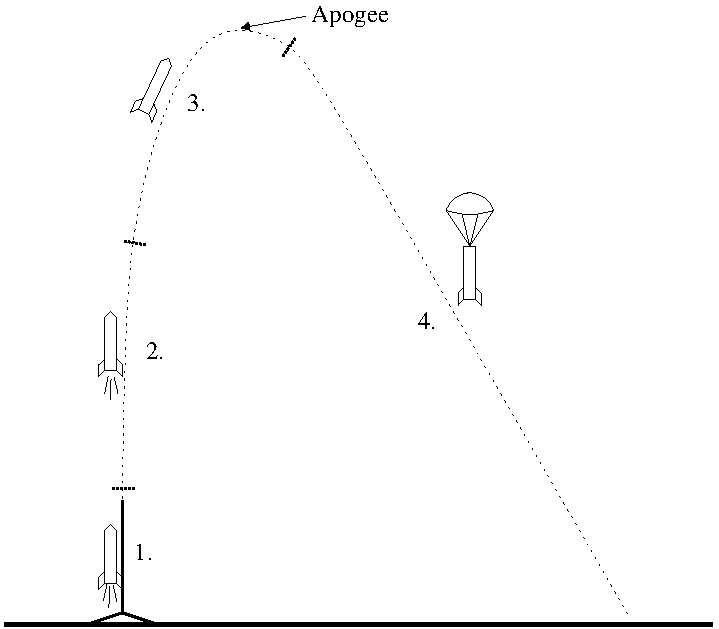
\epsfig{file=figures/model-flight,scale=0.8}
\caption{The basic phases of a typical model rocket flight:
  1.~Launch, 2.~Powered flight, 3.~Coasting and 4.~Recovery.}
\label{fig-model-flight}
\end{figure}

Model rockets are launched from a vertical launch guide that keeps the
rocket in an upright position until it has sufficient velocity for the
fins to aerodynamically stabilize the flight.  The NAR safety code
forbids launching a model rocket at an angle greater than 
$30^\circ$ from vertical.  A typical launch guide for small rockets is
a metal rod about 3-5~mm in diameter, and the launch lug is a short
piece of plastic tube glued to the body tube.  Especially in 
larger rockets this may be replaced by two extruding bolts, the ends
of which slide along a metal rail.  Use of a launch lug can be avoided
by a tower launcher, which has 3--4 metal bars around the rocket
that hold it in an upright position.

After clearing the launch guide, the rocket is in free, powered flight.
During this phase the motor accelerates the rocket while it is
aerodynamically stabilized to keep its vertical orientation.  When the
propellant has been used, the rocket is typically at its maximum
velocity.  It then coasts freely for a short period while the motor
produces smoke to help follow the rocket, but provides no
additional thrust.  Finally, at approximately the point of apogee, a
small pyrotechnical ejection charge is fired upwards from the motor
which pressurizes the model rocket and opens the recovery device.

High-power rocket motors usually have no ejection charges incorporated
in them.  Instead, the rocket carries a small flight computer that
measures the acceleration of the rocket or the outside pressure change
to detect the point of apogee and to open the recovery device.
Frequently only a small drogue parachute is opened at apogee, and the
main parachute is opened at some pre-defined lower altitude around
100--300 meters.

The typical recovery device of a model rocket is either a parachute or
a {\it streamer}.  The parachutes are usually a simple planar circle
of plastic or fabric with 4--10 shroud lines attached.  A streamer is
a strip of plastic or fabric connected to the rocket, intended to
flutter in the air and thus slow down the descent of the rocket.
Especially small rockets often use streamers as their recovery device,
since even light wind can cause a light-weight rocket with a
parachute to drift a significant distance.




\section{Rocket motor classification}
\label{sec-motors}
\label{sec-motor-classes}

The motors used in model and high power rocketry are categorized based
on their total impulse.  A class `A' motor may have a total impulse in
the range of 1.26--2.50~Ns.  Every consecutive class doubles the
allowed total impulse of the motor.  Thus, a B-motor can have an
impulse in the range 2.51--5.00~Ns and a C-motor in the range
5.01--10.0~Ns.  There are also classes \half A and \quarter A which
have impulse ranges half and one quarter of those of an A-motor,
respectively.  Commercial rocket motors are available up to
class~O with a total impulse of 30\s000~Ns~\cite{all-certified-motors}.
Table~\ref{tab-motor-classes} lists the impulse ranges for model
and high-power rocket motors. 

\begin{table}
\caption{Total impulse ranges for motor classes \quarter A--O.}
\label{tab-motor-classes}
\begin{center}
\begin{tabular}{cr@{--}l|cr@{--}l|cr@{--}l}
\hline
\quarter A & 0.0 & 0.625~Ns   & E & 20.01 & 40.0~Ns & K & 1280.01 & 2560~Ns \\
\half A & 0.626 & 1.25~Ns  & F & 40.01 & 80.0~Ns & L & 2560.01 & 5120~Ns \\
A    & 1.26 & 2.50~Ns   & G & 80.01 & 160~Ns  & M & 5120.01 & 10240~Ns \\
B    & 2.51 & 5.00~Ns   & H & 160.01 & 320~Ns   & N & 10240.01 & 20480~Ns \\
C    & 5.01 & 10.0~Ns   & I & 320.01 & 640~Ns   & O & 20480.01 & 40960~Ns \\
D    & 10.01 & 20.0~Ns  & J & 640.01 & 1280~Ns  &  \\
\hline
\end{tabular}
\end{center}
\end{table}

Another important parameter of a rocket motor is the thrust given by
the motor.  This defines the mass that may be lifted by the motor and
the acceleration achieved.  Small model rocket motors typically have
an average thrust of about 3--10~N, while high-power rocket motors can
have thrusts in excess of 5\s000~N.

The third parameter used to classify a model rocket motor is the
length of the delay between the motor burnout and the ignition of the
ejection charge.  Since the maximum velocity of different rockets
using the same type of motor can be vastly different, also the length
of the coasting phase varies.  Therefore motors with otherwise the
same specifications are often manufactured with several different
delay lengths.  These delay lengths do not apply to high-power rocket
motors, since they do not have ejections charges incorporated in them.

Model rocket motors are given a classification code based on these
three parameters, for example ``D7-3''.  The letter specifies the
total impulse range of the motor, while the first number specifies the
average thrust in Newtons and the second number the delay of the
ejection charge in seconds.  The delay number can also be replaced by
`P', which stands for {\it plugged}, \ie the motor does not have an
ejection charge.  Some manufacturers may also use an additional letter
at the end of the classification code specifying the
propellant type used in the motor.

Even motors with the same classification code may have slight
variations to them.  First, the classification only specifies the
impulse range of the motor, not the exact impulse.  In principle, a
D-motor in the lower end of the range might have a total impulse only
1~Ns larger than a C-motor in the upper end of its range.  Second,
the code only specifies the average thrust of the motor.  The thrust
rarely is constant, but varies with time.
Figure~\ref{fig-thrust-curve} shows the typical thrust curve of a
small black powder rocket motor.  The motors typically have a short
thrust peak at ignition that gives the rocket an initial acceleration
boost before stabilizing to a thrust level a little below the average
thrust.  Statically measured thrust curves of most commercial rocket
motors are readily available on the
Internet~\cite{thrust-curve-database}.

\begin{figure}
\centering
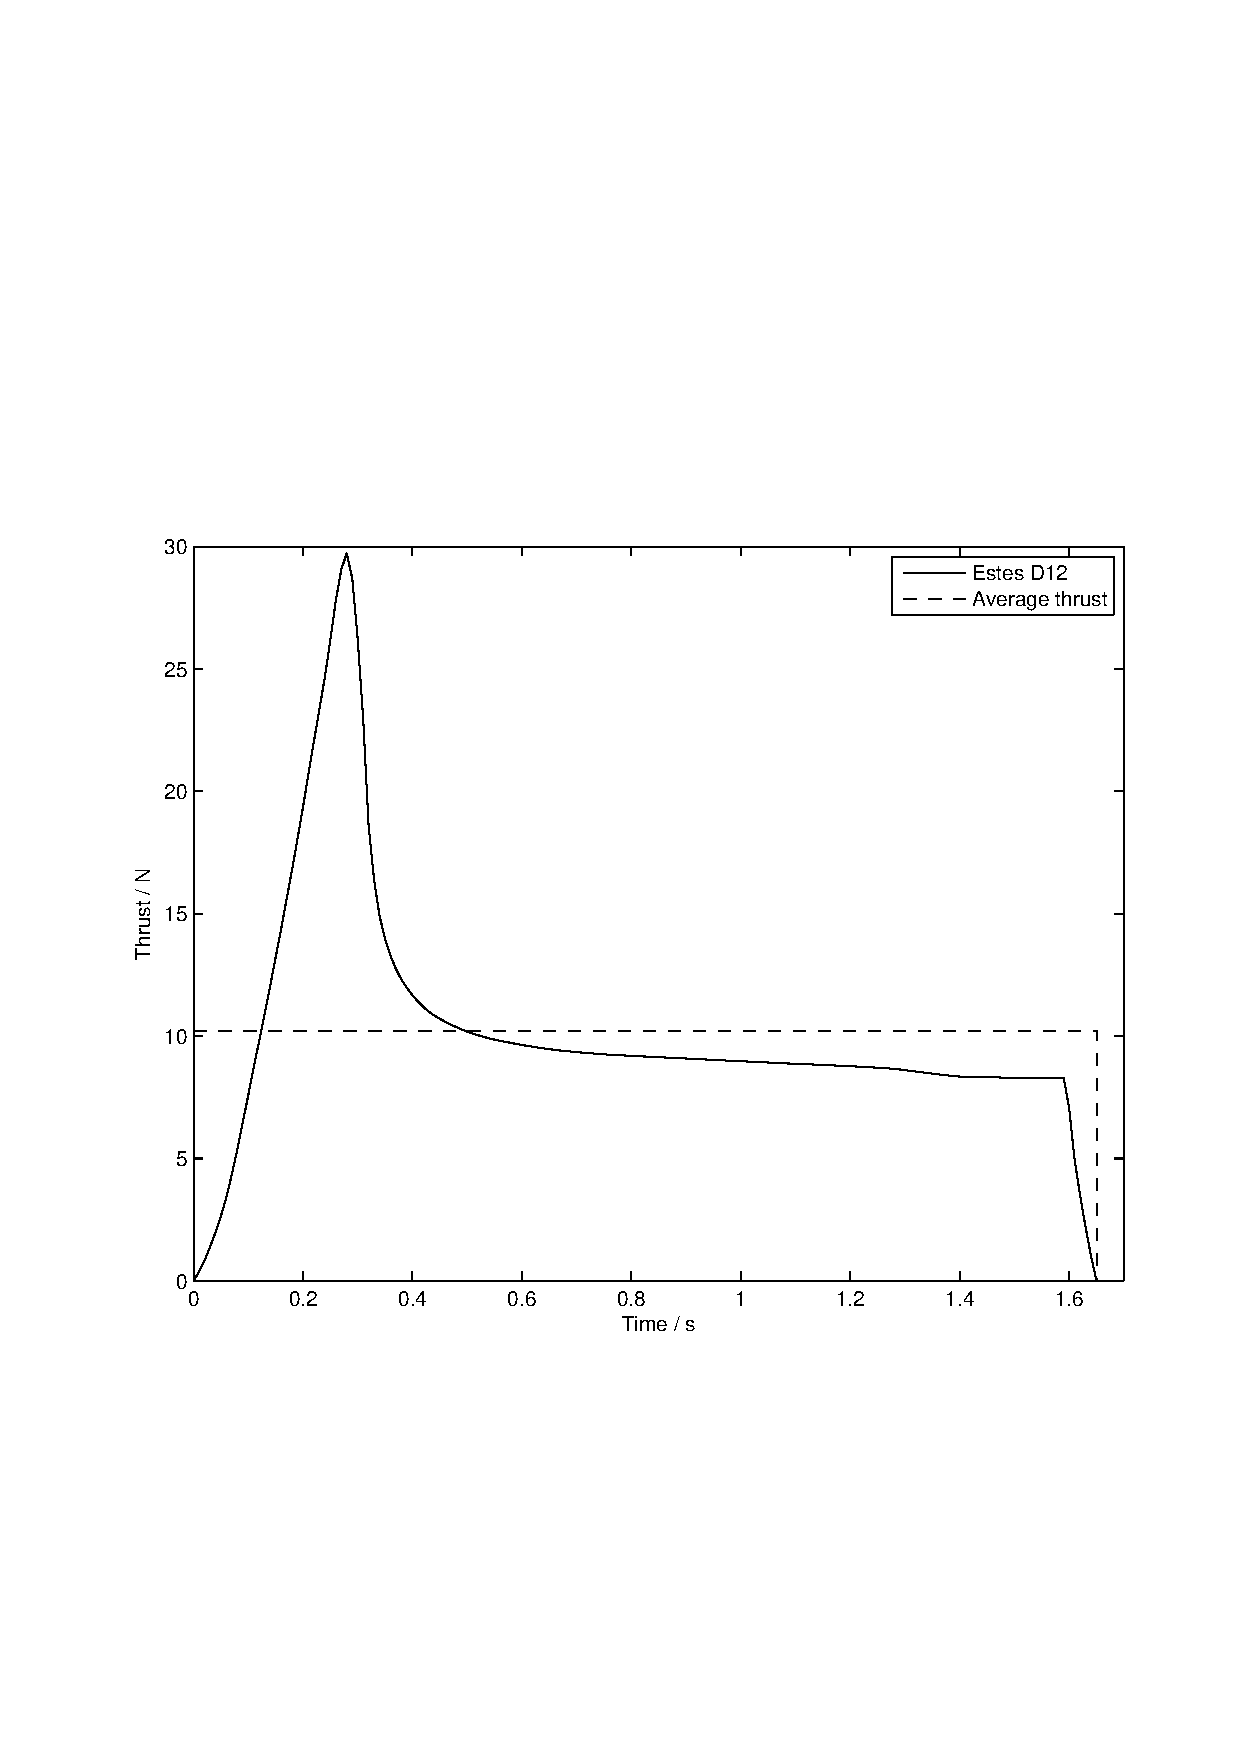
\epsfig{file=figures/motors/D12-thrustcurve,width=9cm}
\caption{A typical thrust curve of an Estes D12-3 rocket motor and
  its average thrust.~\cite{D12-curve}}
\label{fig-thrust-curve}
\end{figure}

Also the propellant type may affect the characteristics of the motor.
Most model rocket motors are made up of a solid, pyrotechnical
propellant---typically black powder---that is cast into a suitable
shape and ignited on launch.  Since the propellant burns on its
surface, different thrust curves can be achieved by different mold
shapes.

% vesiraketit!

A significantly different motor type, {\it hybrid motors}, were
commercially introduced in 1995.  These motors typically include the
propellant and oxidizer in different states, typically a composite
plastic as the fuel and a separate tank of liquid nitrous oxide 
($\rm N_2O$) as the oxidizer.  The plastic on its own does not 
burn very well, but provides ample thrust when the nitrous oxide is
fed through its core.  The nitrous oxide tank is
self-pressurized by its natural vapor pressure. However, since
temperature greatly affects the vapor pressure of nitrous oxide, the
thrust of a hybrid motor is also diminished if the oxidizer is cold.
On the other hand, the motor will burn longer in this case, and since
nitrous oxide is denser when cold, the motor may even yield a greater
total impulse.

The significance of this effect was observed when analyzing the video
footage of the launch of the first Finnish hybrid rocket,
``Haisun��t�''~\cite{haisunaata-launch}.  The average thrust during the
first 0.5~seconds was determined to be only about 70~N, whereas the
static tests suggest the thrust should have been over 200~N.
Instead, the motor burned for over 10~seconds, while the normal thrust
curves indicate a burning time of 5--6~seconds.  This shows that the
temperature of the hybrid motor oxidizer can have a dramatic effect on
the thrust given by the motor, and the static test curve should be
assumed to be valid only in similar operating conditions as during the
test.

One further non-pyrotechnical rocket type is {\it water rockets}.
These are especially popular first rockets, as they require no special
permits and are easy to construct.  The water rocket includes a bottle
or other chamber that has water and pressurized air inside it.  On
launch the pressure forces the water out of a nozzle, providing thrust
to the rocket.  While simulating water rockets is beyond the scope of
this thesis, it is the aim that methods for modeling water rockets can
be added to the produced software in the future.



\section{Clustering and staging}

Two common methods used to achieve greater altitudes with model
rockets are {\it clustering} and {\it staging}.  A cluster has two or
more rocket motors burning concurrently, while staging uses motors
that burn consecutively.  The motor configuration of a cluster and
staged rocket is depicted in Figure~\ref{fig-cluster-stages}.

When a cluster is launched, the total thrust is the sum of the thrust
curves of the separate motors.  This allows greater acceleration and
a greater liftoff weight.  Staging is usually performed by using
zero-delay motors, that ignite the ejection charge immediately at
burnout.  The ejection charge fires towards the upper stage motor and
ignites the next motor.  High power motors with no ejection charges
can be clustered by using an onboard accelerometer or timer that
ignites the subsequent stages.  Staging provides a longer duration of
powered flight, thus increasing the altitude.


\begin{figure}
\centering
\parbox{65mm}{\centering
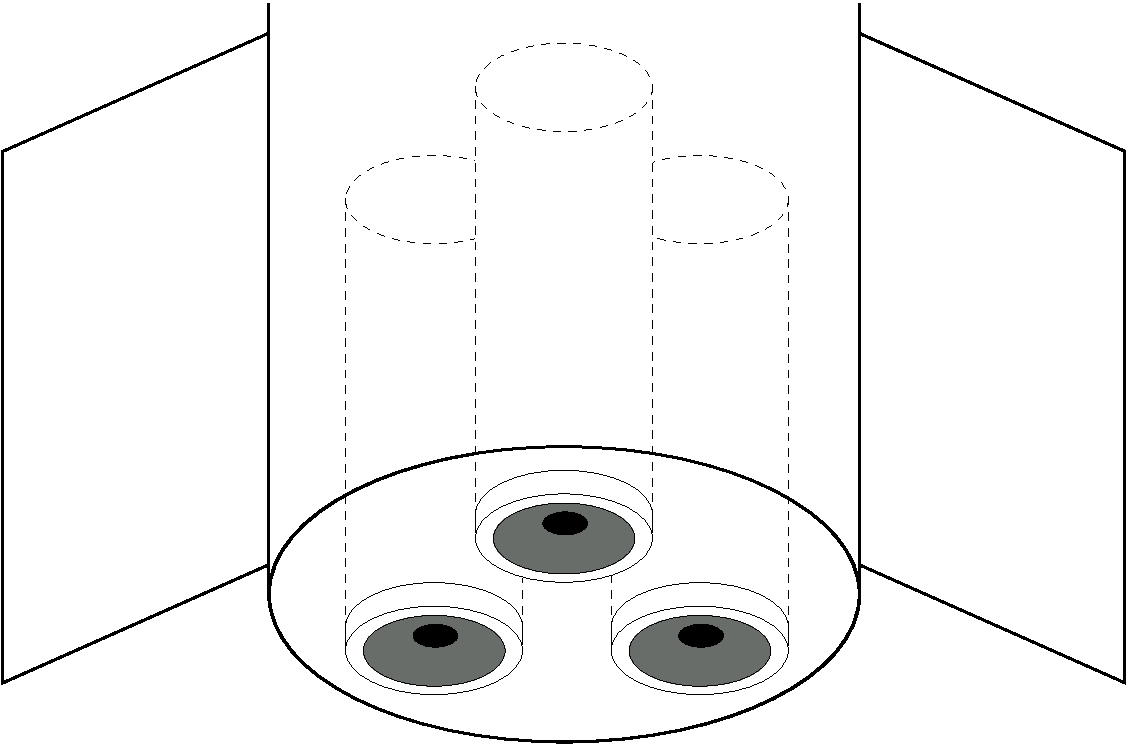
\epsfig{file=figures/motors/cluster,width=60mm} \\ (a)}
\hspace{10mm}
\parbox{40mm}{\centering
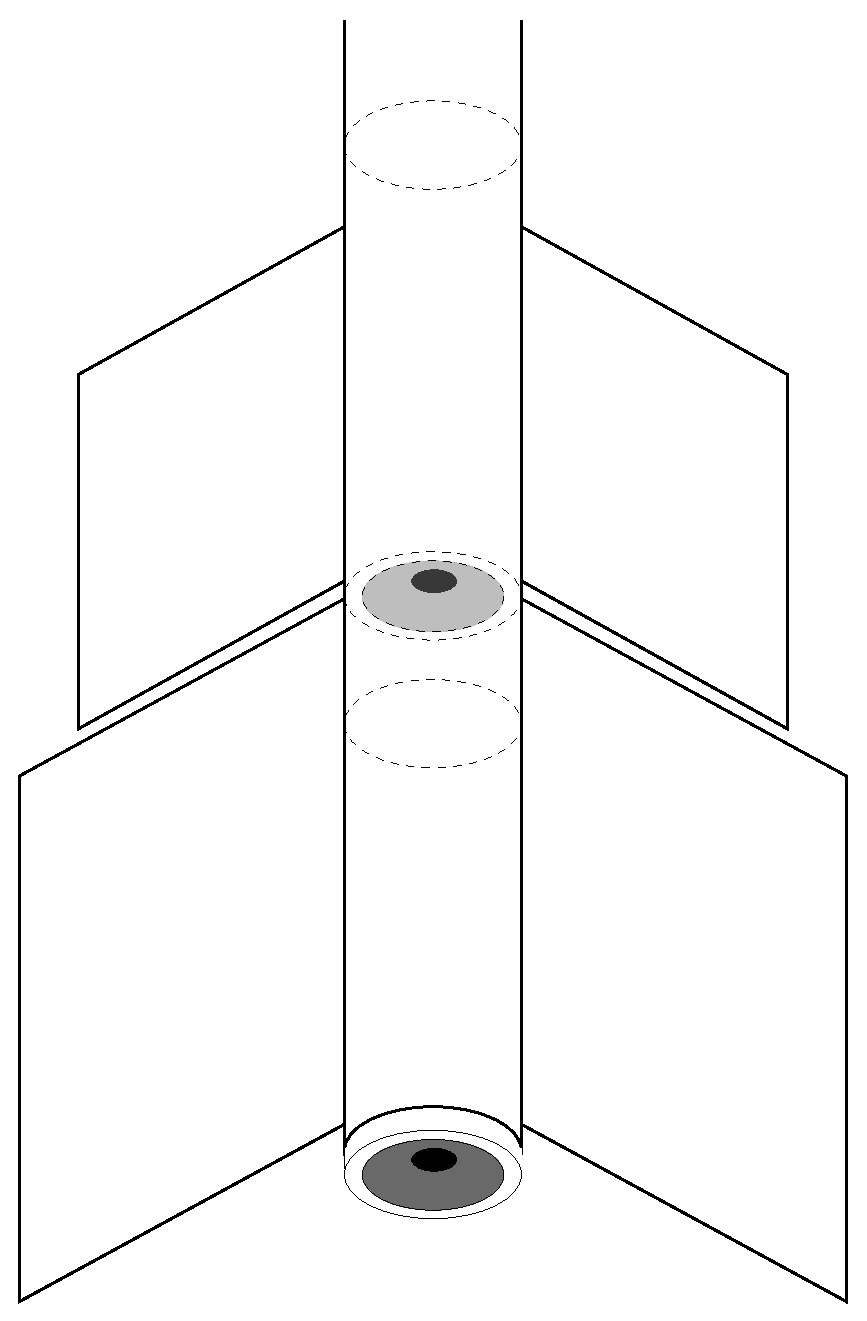
\epsfig{file=figures/motors/staged,width=30mm} \\ (b)}
\caption{The motor configuration for (a) a cluster rocket and (b) a
  two-staged rocket.}
\label{fig-cluster-stages}
\end{figure}

Clustering provides a greater acceleration at launch, but staging
typically provides greater altitude than a cluster with similar
motors.  This is because a clustered rocket accelerates quickly to a
greater speed thus also increasing the aerodynamic drag.  A staged
rocket has a smaller thrust for a longer period of time, which reduces
the overall effect of drag during the flight.


\section{Stability of a rocket}
\label{sec-stability}

When designing a new rocket, its stability is of paramount
importance.  A small gust of wind or some other disturbance may cause
the rocket to tilt slightly from its current orientation.  When this
occurs, the rocket centerline is no longer parallel to the
velocity of the rocket.  This condition is called flying at an 
{\it angle of attack $\alpha$}, where $\alpha$ is the angle between
the rocket centerline and the velocity vector.

When a stable rocket flies at an angle of attack, its fins produce a
moment to correct the rocket's flight.  The corrective moment is
produced by the aerodynamic forces perpendicular to the axis of the
rocket.  Each component of the rocket can be seen as producing a
separate normal force component originating from the component's CP,
as depicted in Figure~\ref{fig-normal-forces}.

\begin{figure}
\centering
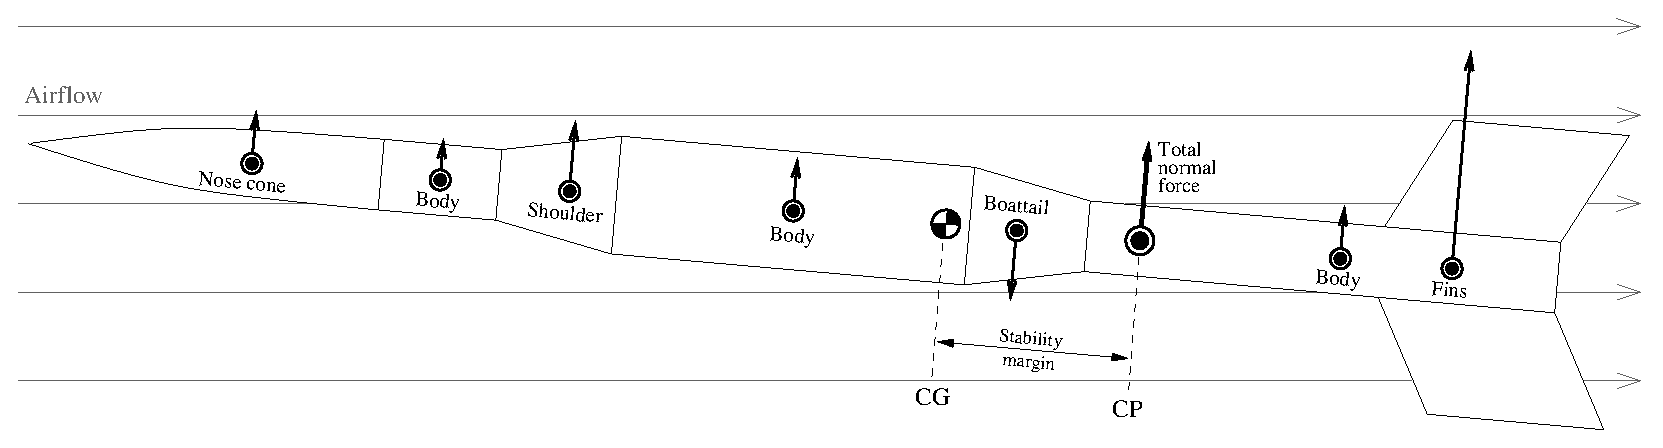
\epsfig{file=figures/aerodynamics/component-normal-forces,width=130mm}
\caption{Normal forces produced by the rocket components.}
\label{fig-normal-forces}
\end{figure}

The effect of the separate normal forces can be combined into a single
force, the magnitude of which is the sum of the separate forces and
which effects the same moment as the separate forces.  The point on
which the total force acts is defined as the center of pressure or the
rocket.  As
can be seen from Figure~\ref{fig-normal-forces}, the moment produced
attempts to correct the rocket's flight only if the CP is located aft
of the CG. If this condition holds, the rocket is said to be 
{\it statically stable}.  A statically stable rocket always produces a
corrective moment when flying at a small angle of attack.  

The argument for static stability above may fail in two conditions:
First, the normal forces might cancel each other out exactly, in which
case a moment would be produced but with zero total force.  Second,
the normal force at the CP might be in the wrong direction (downward
in the figure), yielding an uncorrective moment.  However, we shall
see that the only component to produce a downward force is a boattail,
and the force is equivalent to the corresponding broadening of the
body.  Therefore the total force acting on the rocket cannot be zero
nor in a direction to produce an uncorrective moment when aft of the
CG.

The {\it stability margin} of a rocket is defined as the distance between
the CP and CG, measured in {\it calibers}, where one caliber is the
maximum body diameter of the rocket.  A rule of thumb among model
rocketeers is that the CP should be approximately 1--2 calibers aft of
the CG.  However, the CP of a rocket typically moves upwards as the
angle of attack increases.  In some cases, a 1--2 caliber stability
margin may totally disappear at an angle of attack of only a few
degrees.  As side wind is the primary cause of angles of attack, this
effect is called 
{\it wind caused instability}~\cite{galejs}.

Another stability issue concerning rocketeers is the
{\it dynamic stability} of a rocket.  A rocket that is statically
stable may still be poor at returning the rocket to the original
orientation quickly enough.  Model rockets may encounter several types of
dynamic instability depending on their shape, size and
mass~\cite[pp.~140--141]{stine}:
%
\begin{enumerate}
\item {\it Too little oscillation damping.}  In short, light-weight
  rockets the corrective moment may significantly over-correct the
  perturbation, requiring a corrective moment in the opposite
  direction.  This may lead to continuous oscillation during the
  flight.
\item {\it Too small corrective moment.}  This is the case of over-damped
  oscillation, where the corrective moment is too small compared to
  the moment of inertia of the rocket.  Before the rocket has been
  able to correct its orientation, the thrust of the motors may have
  already significantly affected the direction of flight.
\item {\it Roll-pitch coupling.}  If the model has a natural roll
  frequency (caused \eg by canting the fins) close to the oscillation
  frequency of the rocket, roll-pitch resonance may occur and cause
  the model to go unstable.
\end{enumerate}

By definition, dynamic stability issues are such that they occur over
time during the flight of the rocket.  A full flight simulation that
takes into account all corrective moments automatically also simulates
the possible dynamic stability problems.  Therefore the dynamic
stability of rockets will not be further considered in this
thesis. For an analytical consideration of the problem, refer to
\cite{advanced-model-rocketry}.






\chapter{Aerodynamic properties of model rockets~~}
\label{chap-aerodynamics}

A model rocket encounters three basic forces during its flight:
thrust from the motors, gravity, and aerodynamical forces.  Thrust is
generated by the motors by exhausting high-velocity gases in the
opposite direction.  The thrust of a motor is directly proportional to
the velocity of the escaping gas and the mass per time unit that is
exhausted.  The thrust of commercial model rocket motors as a function
of time have been measured in static motor tests and are readily
available online~\cite{thrust-curve-database}.  Normally the thrust of
a rocket motor is aligned on the center axis of the rocket, so that it
produces no angular moment to the rocket.

Every component of the rocket is also affected by gravitational
force.  When the forces and moments generated are summed up, the
gravitational force can be seen as a single force originating from the
{\it center of gravity} (CG).  A homogeneous gravitational field does
not generate any angular moment on a body relative to the CG.
Calculating the gravitational force is therefore a simple matter of
determining the total mass and CG of the rocket.

Aerodynamic forces, on the other hand, produce both net forces and
angular moments.  To determine the effect of the aerodynamic
forces on the rocket, the total force and moment must be calculated
relative to some reference point.  In this chapter, a method for
determining these forces and moments will be presented.



\section{General aerodynamical properties}
\label{sec-general-aerodynamics}

The aerodynamic forces acting on a rocket are usually split into
components for further examination.  The two most important
aerodynamic force components of interest in a typical model rocket are
the {\it normal force} and {\it drag}.  The aerodynamical normal
force is the force component that generates the corrective moment
around the CG and provides stabilization of the rocket.  The 
drag of a rocket is defined as the force component parallel to the
velocity of the rocket.  This is the aerodynamical force that opposes
the movement of the rocket through air.

Figure~\ref{fig-aerodynamic-forces}(a) shows the thrust, gravity,
normal force and drag of a rocket in free flight.  It should be noted
that if the rocket is flying at an angle of attack $\alpha>0$, then
the normal force and drag are not perpendicular.  In order to have
independent force components, it is necessary to define component
pairs that are always perpendicular to one another.  Two such pairs
are the normal force and axial drag, or side force and drag, shown in
Figure~\ref{fig-aerodynamic-forces}(b).  The two pairs coincide if the
angle of attack is zero.  The component pair that will be used as a
basis for the flight simulations is the normal force and axial drag.


\begin{figure}
\centering
\parbox{35mm}{\centering
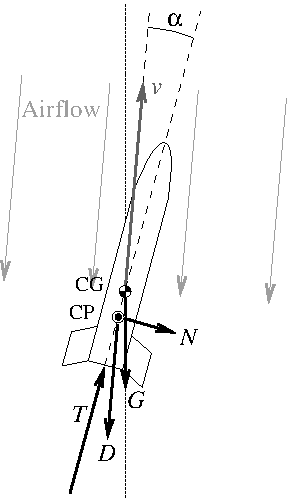
\epsfig{file=figures/aerodynamics/free-flight-forces,width=35mm} \\ (a)}
\hfill
\parbox{35mm}{\centering
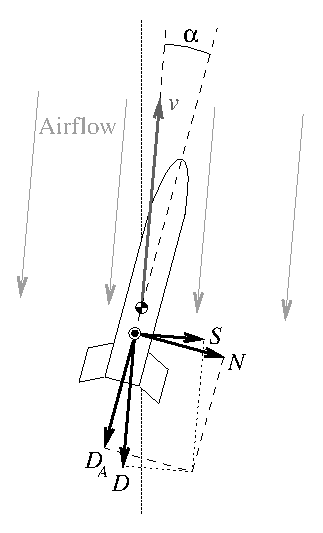
\epsfig{file=figures/aerodynamics/aero-force-components,width=35mm} \\ (b)}
\hfill
\parbox{35mm}{\centering
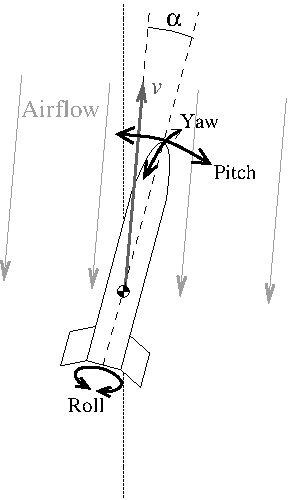
\epsfig{file=figures/aerodynamics/pitch-yaw-roll,width=35mm} \\ (c)}
\caption{(a) Forces acting on a rocket in free flight: gravity $G$,
  motor thrust $T$, drag $D$ and normal force $N$.  (b) Perpendicular
  component pairs of the total aerodynamical force: normal force $N$
  and axial drag $D_A$; side force $S$ and drag $D$.  (c) The pitch,
  yaw and roll directions of a model rocket.}
\label{fig-aerodynamic-forces}
\end{figure}


The three moments around the different axis are called the 
{\it pitch}, {\it yaw} and {\it roll moments}, as depicted in
Figure~\ref{fig-aerodynamic-forces}(c).  Since a typical rocket has no
``natural'' roll angle of flight as an aircraft does, we may choose
the pitch angle to be in the same plane as the angle of attack, \ie
the plane defined by the velocity vector and the centerline of the
rocket.  Thus, the normal force generates the pitching moment and no
other moments.





\subsection{Aerodynamic force coefficients}

When studying rocket configurations, the absolute force values are
often difficult to interpret, since many factors affect them.  In
order to get a value better suited for comparison, the forces are
normalized by the current dynamic pressure $q=\frac{1}{2}\rho v_0^2$
and some characteristic area \Aref\ to get a non-dimensional force
coefficient. Similarly, the moments are normalized by the dynamic
pressure, characteristic area and characteristic length $d$.  Thus,
the normal force coefficient corresponding to the normal force $N$ is
defined as
%
\begin{equation}
C_N  =  \frac{N}{\frac{1}{2}\rho v_0^2 \, \Aref} 
\label{eq-CN-def}
\end{equation}
%
and the pitch moment coefficient for a pitch moment $m$ as
%
\begin{equation}
C_m  =  \frac{m}{\frac{1}{2}\rho v_0^2 \, \Aref\, d}.
\label{eq-Cm-def}
\end{equation}
%
A typical choice of reference area is the base of the rocket's nose
cone and the reference length is its diameter.

The pitch moment is always calculated around some reference point,
while the normal force stays constant regardless of the point of
origin.  If the moment coefficient $C_m$ is known for some reference
point, the moment coefficient at another point $C_m'$ can be
calculated from
%
\begin{equation}
C_m'd = C_md - C_N\Delta x
\label{eq-moment-reference}
\end{equation}
%
where $\Delta x$ is the distance along the rocket centerline.
Therefore it is sufficient to calculate the moment coefficient only at
some constant point along the rocket body.  In this thesis the
reference point is chosen to be the tip of the nose cone.

The {\it center of pressure} (CP) is defined as the position from
which the total normal force alone produces the current pitching
moment.  Therefore the total normal force produces no moment around
the CP itself, and an equation for the location of the CP
can be obtained from (\ref{eq-moment-reference}) by selecting setting
$C_m'=0$:
%
\begin{equation}
X = \frac{C_m}{C_N}\,d
\end{equation}
%
Here $X$ is the position of the CP along the rocket centerline from
the nose cone tip.  This equation is valid when $\alpha>0$.  As
$\alpha$ approaches zero, both $C_m$ and $C_N$ approach zero.  The CP
is then obtained as a continuous extension using l'H�pital's rule
%
\begin{equation}
X = \left.\frac{\;\frac{\partial C_m}{\partial\alpha}\;}
          {\;\frac{\partial C_N}{\partial\alpha}\;}\,d\right|_{\alpha=0}
  = \frac{\Cma}{\CNa}\,d
\label{eq-CP-position}
\end{equation}
%
where the normal force coefficient and pitch moment coefficient
derivatives have been defined as
%
\begin{equation}
\CNa = \left.\frac{\partial C_N}{\partial\alpha}\right|_{\alpha=0}
\hspace{5mm}\mbox{and}\hspace{5mm}
\Cma = \left.\frac{\partial C_m}{\partial\alpha}\right|_{\alpha=0}.
\label{eq-CNa-derivative}
\end{equation}

At very small angles of attack we may approximate $C_N$ and $C_m$ to
be linear with $\alpha$, so to a first approximation
%
\begin{equation}
C_N \approx \CNa\,\alpha
\hspace{5mm}\mbox{and}\hspace{5mm}
C_m \approx \Cma\,\alpha.
\label{eq-CNa-approx}
\end{equation}
%
The Barrowman method uses the coefficient derivatives to determine the
CP position using equation~(\ref{eq-CP-position}).  However, there are
some significant nonlinearities in the variation of $C_N$ as a
function of $\alpha$.  These will be accounted for by holding the
approximation of equation~(\ref{eq-CNa-approx}) exact and letting
\CNa\ and \Cma\ be a function of $\alpha$.  Therefore, for the
purposes of this thesis we define
%
\begin{equation}
\CNa = \frac{C_N}{\alpha}
\hspace{5mm}\mbox{and}\hspace{5mm}
\Cma = \frac{C_m}{\alpha}
\label{eq-CNa-definition}
\end{equation}
%
for $\alpha>0$ and by equation~(\ref{eq-CNa-derivative}) for
$\alpha=0$.  These definitions are compatible, since
equation~(\ref{eq-CNa-definition}) simplifies to the partial
derivative~(\ref{eq-CNa-derivative}) at the limit
$\alpha\rightarrow0$.  This definition also allows us to stay true to
Barrowman's original method which is familiar to many rocketeers.


Similar to the normal force coefficient, the drag coefficient is
defined as
%
\begin{equation}
C_D = \frac{D}{\frac{1}{2}\rho v_0^2 \, \Aref}.
\label{eq-CD-def}
\end{equation}
%
Since the size of the rocket has been factored out, the drag
coefficient at zero angle of attack $C_{D0}$ allows a straightforward
method of comparing the effect of different rocket shapes on drag.
However, this coefficient is not constant and will vary with \eg the
speed of the rocket and its angle of attack.


If each of the fins of a rocket are canted at some angle $\delta>0$
with respect to the rocket centerline, the fins will produce a roll
moment on the rocket.  Contrary to the normal force and pitching
moment, canting the fins will produce a non-zero rolling moment but no
corresponding net force.  Therefore the only quantity computed is the
roll moment coefficient, defined by
%
\begin{equation}
C_l  =  \frac{l}{\frac{1}{2}\rho v_0^2 \, \Aref\, d}
\label{eq-Cl-def}
\end{equation}
%
where $l$ is the roll moment.

It shall be shown later that rockets with axially-symmetrical fin
configurations experience no forces that would produce net yawing
moments. However, a single fin may produce all six types of forces and
moments. The equations for the forces and moments of a single fin will
not be explicitly written out, and they can be computed from the
geometry in question.



\subsection{Velocity regions}

Most of the aerodynamic properties of rockets vary with the velocity
of the rocket.  The important parameter is the {\it Mach number},
which is the free-stream velocity of the rocket divided by the local
speed of sound
%
\begin{equation}
M = \frac{v_0}{c}.
\end{equation}
%
The velocity range encountered by rockets is divided into regions with
different impacts on the aerodynamical properties, listed in
Table~\ref{tab-sonics}.  

In {\it subsonic flight} all of the airflow around the rocket occurs
below the speed of sound.  This is the case for approximately $M<0.8$.
At very low Mach numbers air can be effectively treated as an
incompressible fluid, but already above $M\approx 0.3$ some
compressibility issues may have to be considered.

In {\it transonic flight} some of the air flowing around the rocket
accelerates above the speed of sound, while at other places it remains
subsonic.  Some local shock waves are generated and hard-to-predict
interference effects may occur.  The drag of a rocket has a sharp
increase in the transonic region, making it hard to pass into the
supersonic region.  Transonic flight occurs at Mach numbers of
approximately 0.8--1.2.

In {\it supersonic flight} all of the airflow is faster than the
speed of sound (with the exception of \eg the nose cone tip).  A shock
wave is generated by the nose cone and fins.  In supersonic flight
the drag reduces from that of transonic flight, but is generally
greater than that of subsonic flight.  Above approximately Mach 5 new
phenomena begin to emerge that are not encountered at lower supersonic
speeds. This region is called {\it hypersonic flight}.

\begin{table}
\caption{Velocity regions of rocket flight}
\label{tab-sonics}
\begin{center}
\begin{tabular}{cr@{ -- }l}
Region & \multicolumn{2}{c}{Mach number ($M$)} \\
\hline
Subsonic   & \hspace{10mm} 0   & 0.8 \\
Transonic & 0.8 & 1.2 \\
Supersonic & 1.2 & $\sim5$ \\
Hypersonic & $\sim5$ & \\
\hline
\end{tabular}
\end{center}
\end{table}


Methods for predicting the aerodynamic properties of subsonic flight
and some extensions to supersonic flight will be presented.  Since the
analytical prediction of aerodynamic properties in the transonic
region is quite difficult, this region will be accounted for by using
some suitable interpolation function that corresponds reasonably to
actual measurements. Hypersonic flight will not be considered, since
practically no model or high power rockets ever achieve such speeds.


\subsection{Flow and geometry parameters}

There exist many different parameters that characterize aspects of
flow or a rocket's geometry.  One of the most important flow
parameters is the {\it Reynolds number} $R$.  It is a dimensionless
quantity that characterizes the ratio of inertial forces and viscous
forces of flow.  Many aerodynamic properties depend on the Reynolds
number, defined as
%
\begin{equation}
R = \frac{v_0\; L}{\nu}.
\end{equation}
%
Here $v_0$ is the free-stream velocity of the rocket, $L$ is a
characteristic length and $\nu$ is the kinematic viscosity of air.  It
is notable that the Reynolds number is dependent on a characteristic
length of the object in question. In most cases, the length used is
the length of the rocket.  A typical 30~cm sport model flying at
50~m/s has a corresponding Reynolds number of approximately
1\s000\s000.

Another term that is frequently encountered in aerodynamical equations
has been defined its own parameter $\beta$, which characterizes the
flow speed both in subsonic and supersonic flow:
%
\begin{equation}
\beta = \sqrt{\envert{M^2-1}} =
\left\{
\begin{array}{ll}
\sqrt{1-M^2}, & {\rm if\ } M<1 \\
\sqrt{M^2-1}, & {\rm if\ } M>1
\end{array}
\right.
\end{equation}
%
As the flow speed approaches the transonic region $\beta$ approaches
zero.  This term appears for example in the {\it Prandtl factor} $P$
which corrects subsonic force coefficients for compressible flow:
%
\begin{equation}
P = \frac{1}{\beta} = \frac{1}{\sqrt{1-M^2}}
\label{eq-prandtl-factor}
\end{equation}

It is also often useful to define parameters characterizing general
properties of a rocket.  One such parameter is the {\it caliber},
defined as the maximum body diameter.  The caliber is often used to
indicate relative distances on the body of a rocket, such as the
stability margin.  Another common parameter characterizes the
``slenderness'' of a rocket.  It is the {\it fineness ratio} of a
rocket $f_B$, defined as the length of the rocket body divided by the
maximum body diameter.  Typical model rockets have a fineness ratio in
the range of 10--20, but extreme models may have a fineness ratio as
low as 5 or as large as 50.




\subsection{Coordinate systems}

During calculation of the aerodynamic properties a coordinate system
fixed to the rocket will be used.  The origin of the coordinates is at
the nose cone tip with the positive $x$-axis directed along the rocket
centerline.  This convention is also followed internally in the
produced software.  In the following sections the position of the $y$-
and $z$-axes are arbitrary; the parameter $y$ is used as a general
spanwise coordinate when discussing the fins.  During simulation,
however, the $y$- and $z$-axes are fixed in relation to the rocket,
and do not necessarily align with the plane of the pitching moments.



\clearpage
\section{Normal forces and pitching moments}

Barrowman's method~\cite{barrowman-thesis} for determining the total
normal force coefficient derivative \CNa, the pitch moment
coefficient derivative \Cma\ and the CP location at subsonic speeds
first splits the rocket into simple separate components, then
calculates the CP location and \CNa\ for each component separately and
then combines these to get the desired coefficients and CP
location.  The general assumptions made by the derivation are:
%
\begin{enumerate}
\item The angle of attack is very close to zero.
\item The flow around the body is steady and non-rotational.
\item The rocket is a rigid body.
\item The nose tip is a sharp point.
\item The fins are flat plates.
\item The rocket body is axially symmetric.
\end{enumerate}

The components that will be discussed are nose cones, cylindrical body
tube sections, shoulders, boattails and fins, in an arbitrary
order.  The interference effect between the body and fins will be
taken into account by a separate correction term.  Extensions to
account for body lift and arbitrary fin shapes will also be derived.


\subsection{Axially symmetric body components}

The body of the rocket is assumed to be an axially symmetric body of
rotation.  The entire body could be considered to be a single
component, but in practice it is divided into nose cones, shoulders,
boattails and cylindrical body tube sections.  The geometry of typical
nose cones, shoulders and boattails are described in
Appendix~\ref{app-nosecone-geometry}.

The method presented by Barrowman for calculating the normal force and
pitch moment coefficients at supersonic speeds is based on a
second-order shock expansion method.  However, this assumes that the
body of the rocket is very streamlined, and it cannot handle areas
with a slope larger than than $\sim30^\circ$.  Since the software
allows basically any body shape, applying this method would be
difficult.

Since the emphasis is on subsonic flow, for the purposes of this
thesis the normal force and pitching moments produced by the body are
assumed to be equal at subsonic and supersonic speeds.  The assumption
is that the CP location is primarily affected by the fins.  The effect
of supersonic flight on the drag of the body will be accounted for in
Section~\ref{sec-drag}.



\subsubsection{\CNa\ of body components at subsonic speeds}

The normal force for an axially symmetric body at position $x$ in
subsonic flow is given by
%
\begin{equation}
N(x) = \rho v_0 \; \frac{\partial}{\partial x}[A(x)w(x)]
\label{eq-normal-force}
\end{equation}
%
where $A(x)$ is the cross-sectional area of the body, and the $w(x)$
is the local downwash, given as a function of the angle of attack as
%
\begin{equation}
w(x) = v_0 \sin\alpha.
\end{equation}
%
For angles of attack very close to zero $\sin\alpha\approx\alpha$, but
contrary to the original derivation, we shall not make this
simplification.  From the definition of the normal force
coefficient~(\ref{eq-CN-def}) and equation~(\ref{eq-normal-force}) we
obtain
%
\begin{equation}
C_N(x) = \frac{N(x)}{\frac{1}{2}\rho v_0^2\;\Aref}
       = \frac{2\; \sin\alpha}{\Aref}\; \frac{\dif A(x)}{\dif x}.
\label{eq-CNx}
\end{equation}
%
Assuming that the derivative $\frac{\dif A(x)}{\dif x}$ is
well-defined, we can integrate over the component length $l$ to obtain
%
\begin{equation}
C_N = \frac{2\; \sin\alpha}{\Aref}\;
      \int_0^l \frac{\dif A(x)}{\dif x}\dif x
    = \frac{2\; \sin\alpha}{\Aref}\; [A(l)-A(0)].
\end{equation}
%
We then have
%
\begin{equation}
\CNa = \frac{C_N}{\alpha}
     = \frac{2}{\Aref}\; [A(l)-A(0)]\;
       \underbrace{\frac{\sin\alpha}{\alpha}}_
  {\parbox{10mm}{\scriptsize\centering
  $\rightarrow 1$ as \\ $\alpha\rightarrow0$}}.
\label{eq-body-CNa}
\end{equation}
%
This is the same equation as derived by Barrowman with the exception
of the correction term $\sin\alpha/\alpha$.

Equation~(\ref{eq-body-CNa}) shows that as long as the cross-sectional
area of the component changes smoothly, the normal force coefficient
derivative does not depend on the component shape, only the difference
of the cross-sectional area at the beginning and end.  As a
consequence, according to Barrowman's theory, a cylindrical body tube
has no effect on the normal force coefficient or CP location.
However, the lift due to cylindrical body tube sections has been noted
to be significant for long, slender rockets even at angles of attack
of only a few degrees~\cite{galejs}.  An extension
for the effect of body lift will be given shortly.




\subsubsection{\Cma\ of body components at subsonic speeds}

A normal force $N(x)$ at position $x$ produces a pitching moment
%
\begin{equation}
m(x) = xN(x).
\end{equation}
%
at the nose cone tip.  Therefore the pitching moment coefficient is
%
\begin{equation}
C_m(x) = \frac{m(x)}{\frac{1}{2}\rho v_0^2\;\Aref\, d}
       = \frac{xN(x)}{\frac{1}{2}\rho v_0^2\;\Aref\, d}.
\end{equation}
%
Substituting equation~(\ref{eq-CNx}) we obtain
%
\begin{equation}
C_m(x) = \frac{x\;C_N(x)}{d}
       = \frac{2\; \sin\alpha\; x}{\Aref\, d}\; \frac{\dif A(x)}{\dif x}.
\end{equation}
%
This can be integrated over the length of the body to obtain
%
\begin{equation}
C_m = \frac{2\;\sin\alpha}{\Aref\,d}
        \int_0^l x \left(\od{A(x)}{x}\right) \dif x
    = \frac{2\;\sin\alpha}{\Aref\,d}
        \sbr{ lA(l)-\int_0^l A(x) \dif x }.
\end{equation}
%
The resulting integral is simply the volume of the body $V$.
Therefore we have
%
\begin{equation}
C_m = \frac{2\;\sin\alpha}{\Aref\,d} \sbr{ lA(l)-V }
\end{equation}
%
and
%
\begin{equation}
\Cma = \frac{2}{\Aref\,d}\sbr{ lA(l)-V }\; \frac{\sin\alpha}{\alpha}.
\label{eq-body-Cma}
\end{equation}
%
This is, again, the result derived by Barrowman with the additional
correction term $\sin\alpha/\alpha$.


\subsubsection{Effect of body lift}
\label{sec-body-lift}

The analysis thus far has neglected the effect of body lift as
negligible at small angles of attack.  However, in the flight of long,
slender rockets the lift may be quite significant at angles of attack
of only a few degrees, which may occur at moderate wind
speeds~\cite{galejs}.

Robert Galejs suggested adding a correction term to the body
component \CNa\ to account for body lift~\cite{galejs}.  The normal
force exerted on a cylindrical body at an angle of attack $\alpha$
is~\cite[p.~3-11]{hoerner}
%
\begin{equation}
C_N = K\; \frac{A_{\rm plan}}{\Aref}\; \sin^2\alpha
\end{equation}
%
where $A_{\rm plan} = d\cdot l$ is the planform area of the cylinder
and K is a constant $K\approx 1.1$.  Galejs had simplified the
equation with $\sin^2\alpha\approx\alpha^2$, but this shall not be
performed here.  At small angles of attack, when the approximation is
valid, this yields a linear correction to the value of \CNa.

It is assumed that the lift on non-cylindrical components can be
approximated reasonably well with the same equation.  The CP location
is assumed to be the center of the planform area, that is
%
\begin{equation}
X_{\rm lift} = \frac{\int_0^l x\; 2r(x)\dif x}{A_{\rm plan}}.
\end{equation}
%
This is reminiscent of the CP of a rocket flying at an angle of attack
of $90^\circ$.  For a cylinder the CP location is at the center of the
body, which is also the CP location obtained at the limit with
equation~(\ref{eq-body-CP-position}).  However, for nose cones,
shoulders and boattails it yields a slightly different position than
equation~(\ref{eq-body-CP-position}).

%The value of $K$ has been experimentally fitted to experimental data
%from wind tunnels.






\subsubsection{Center of pressure of body components}

The CP location of the body components can be calculated by
inserting equations~(\ref{eq-body-CNa}) and (\ref{eq-body-Cma}) into
equation~(\ref{eq-CP-position}):
%
\begin{equation}
X_B = \frac{(\Cma)_B}{(\CNa)_B}\;d
    = \frac{lA(l)-V}{A(l)-A(0)}
\label{eq-body-CP-position}
\end{equation}
%
It is worth noting that the correction term $\sin\alpha/\alpha$
cancels out in the division, however, it is still present in the
value of \CNa\ and is therefore significant at large angles of attack.

The whole rocket body could be numerically integrated and the
properties of the whole body computed.  However, it is often more
descriptive to split the body into components and calculate the
parameters separately.  The total CP location can be calculated from
the separate CP locations $X_i$ and normal force coefficient
derivatives $(\CNa)_i$ by the moment sum
%
\begin{equation}
X = \frac{\sum_{i=1}^n X_i(\CNa)_i}{\sum_{i=1}^n (\CNa)_i}.
\label{eq-moment-sum}
\end{equation}
%
In this manner the effect of the separate components can be more
easily analyzed.



\subsection{Planar fins}
\label{sec-planar-fins}

The fins of the rocket are considered separately from the body.  Their
CP location and normal force coefficient are determined and added to
the total moment sum~(\ref{eq-moment-sum}).  The interference between
the fins and the body is taken into account by a separate correction
term.

In addition to the corrective normal force, the fins can induce a roll
rate if each of the fins are canted at an angle $\delta$.  The roll
moment coefficient will be derived separately in
Section~\ref{sec-roll-dynamics}.

Barrowman's original report and thesis derived the equations for
trapezoidal fins, where the tip chord is parallel to the body
(Figure~\ref{fig-fin-geometry}(a)).  The equations can be extended to
\eg elliptical fins~\cite{barrowman-elliptical-fins}
(Figure~\ref{fig-fin-geometry}(b)), but many model rocket fin
designs depart from these basic shapes.  Therefore an
extension is presented that approximates the aerodynamical
properties for a free-form fin defined by a list of $(x,y)$
coordinates (Figure~\ref{fig-fin-geometry}(c)). 


\begin{figure}
\centering
\parbox{35mm}{\centering
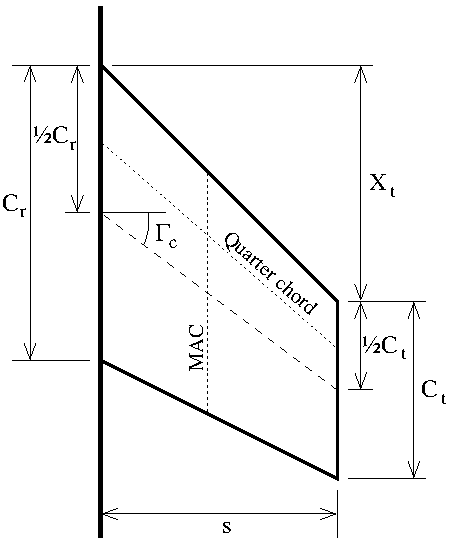
\epsfig{file=figures/fin-geometry/fin-trapezoidal,scale=0.5} \\ (a)}
\hfill
\parbox{35mm}{\centering
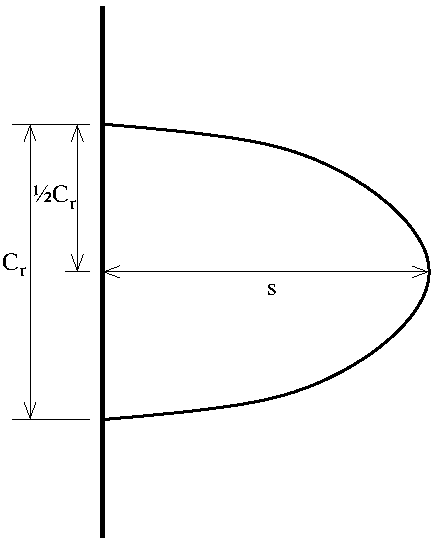
\epsfig{file=figures/fin-geometry/fin-elliptical,scale=0.5} \\ (b)}
\hfill
\parbox{35mm}{\centering
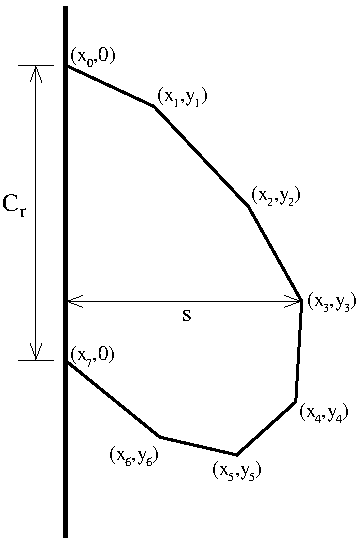
\epsfig{file=figures/fin-geometry/fin-free,scale=0.5} \\ (c)}
\caption{Fin geometry of (a) a trapezoidal fin, (b) an elliptical fin
  and (c) a free-form fin.}
\label{fig-fin-geometry}
\end{figure}



Additionally, Barrowman considered only cases with three or four
fins.  This shall be extended to allow for any reasonable number of
fins, even single fins.


\subsubsection{Center of pressure of fins at subsonic and supersonic
  speeds}

Barrowman argued that since the CP of a fin is located along its mean
aerodynamic chord (MAC) and on the other hand at low subsonic speeds
on its quarter chord, then the CP must be located at the intersection
of these two (depicted in Figure~\ref{fig-fin-geometry}(a)).  He
proceeded to calculate this intersection point analytically from the
fin geometry of a trapezoidal fin.

Instead of following the derivation Barrowman used, an alternative
method will be presented that allows simpler extension to free-form
fins.  The two methods yield identical results for trapezoidal fins.
The length of the MAC $\bar c$, its spanwise position $y_{\rm MAC}$,
and the effective leading edge location $x_{\rm MAC,LE}$ are given
by~\cite{appl-comp-aero-fins}
%
\begin{align}
\bar c &=  \frac{1}{\Afin} \int_0^s c^2(y) \dif y
   \label{eq-MAC-length} \\
y_{\rm MAC} &= \frac{1}{\Afin} \int_0^s yc(y) \dif y 
   \label{eq-MAC-ypos} \\
x_{\rm MAC,LE} &= \frac{1}{\Afin} \int_0^s x_{\rm LE}(y)c(y) \dif y
   \label{eq-MAC-xpos}
\end{align}
%
where $\Afin$ is the one-sided area of a single fin, $s$ is the span of
one fin, and $c(y)$ is the length of the fin chord and $x_{\rm LE}(y)$
the leading edge position at spanwise position $y$.

When these equations are applied to trapezoidal fins and the
lengthwise position of the CP is selected at the quarter chord,
$X_f=x_{\rm MAC,LE}+0.25\,\bar c$,
one recovers exactly the results derived by Barrowman:
%
\begin{align}
y_{\rm MAC} &= \frac{s}{3}\,\frac{C_r+2C_t}{C_r+C_t} \\
X_f &= \frac{X_t}{3}\,\frac{C_r+2C_t}{C_r+C_t} +
          \frac{1}{6}\,\frac{C_r^2+C_t^2+C_rC_t}{C_r+C_t}
\end{align}
%
However, equations~(\ref{eq-MAC-length})--(\ref{eq-MAC-xpos}) may also
be directly applied to elliptical or free-form fins.

Barrowman's method assumes that the lengthwise position of the CP
stays at a constant 25\% of the MAC at subsonic speeds.  However, the
position starts moving rearward above approximately Mach 0.5.  For
$M>2$ the relative lengthwise position of the CP is given by an empirical
formula~\cite[p.~33]{fleeman}
%
\begin{equation}
\frac{X_f}{\bar c} = \frac{\AR\beta - 0.67}{2\AR\beta-1}
\label{eq-fin-CP-mach2}
\end{equation}
%
where $\beta=\sqrt{M^2-1}$ for $M>1$ and \AR\ is the aspect ratio of
the fin defined using the span $s$ as $\AR=2s^2/\Afin$. 
%
Between Mach 0.5 and 2 the lengthwise position of the CP is
interpolated.  A suitable function that gives a curve similar to that
of Figure~2.18 of reference~\cite[p.~33]{fleeman} was found to be a
fifth order polynomial $p(M)$ with the constraints
%
\begin{equation}
  \begin{split}
p(0.5)   & =  0.25 \\
p'(0.5)  & =  0 \\
p(2)     & =  f(2)  \\
p'(2)    & =  f'(2) \\
p''(2)   & =  0 \\
p'''(2)  & =  0
  \end{split}
\end{equation}
%
where $f(M)$ is the function of equation~(\ref{eq-fin-CP-mach2}).



The method presented here can be used to estimate the CP location of
an arbitrary thin fin.  However, problems arise with the method if the
fin shape has a jagged edge as shown in
Figure~\ref{fig-fin-jagged}(a).  If $c(y)$ would include only the sum
of the two separate chords in the area containing the gap, then the
equations would yield the same result as for a fin shown in
Figure~\ref{fig-fin-jagged}(b).  This clearly would be incorrect,
since the position of the latter fin portion would be neglected.  To
overcome this problem, $c(y)$ is chosen as the length from the leading
edge to the trailing edge of the fin, effectively adding the portion
marked by the dotted line to the fin.  This corrects the CP position
slightly rearwards.  The fin area used in
equations~(\ref{eq-MAC-length})--(\ref{eq-MAC-xpos}) must in this case
also be calculated including this extra fin area, but the extra area
must not be included when calculating the normal force coefficient.

This correction is also approximate, since in reality such a jagged
edge would cause some unknown interference factor between the two fin
portions.  Simulating such jagged edges using these methods should
therefore be avoided.


\begin{figure}
\centering
\parbox{35mm}{\centering
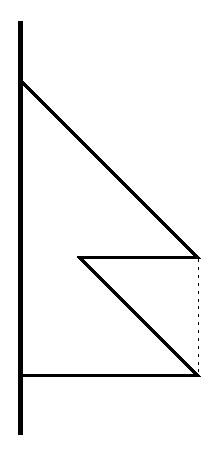
\epsfig{file=figures/fin-geometry/fin-jagged,scale=0.5} \\ (a)}
\hspace{5mm}
\parbox{35mm}{\centering
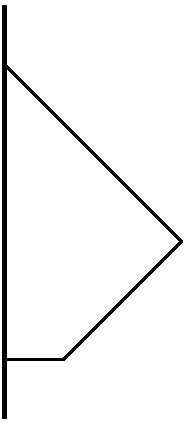
\epsfig{file=figures/fin-geometry/fin-jagged-equivalent,scale=0.5} \\ (b)}
\caption{(a) A jagged fin edge, and (b) an equivalent fin if $c(y)$ is
  chosen to include only the actual fin area.}
\label{fig-fin-jagged}
\end{figure}







\subsubsection{Single fin \CNa\ at subsonic speeds}
\label{sec-average-angle}

Barrowman derived the normal force coefficient derivative value based
on Diederich's semi-empirical method~\cite{diederich}, which states that
for one fin
%
\begin{equation}
\del{\CNa}_1 = \frac{\CNa_0\; F_D \left(\frac{\Afin}{\Aref}\right)
                     \cos\Gamma_c}
             {2+F_D\sqrt{1+\frac{4}{F_D^2}}},
\label{eq-fin-CNa-base}
\end{equation}
%
where
%
\begin{itemize}
\item[$\CNa_0$] = normal force coefficient derivative of a 2D airfoil
\item[$F_D$] = Diederich's planform correlation parameter
\item[$\Afin$] = area of one fin
\item[$\Gamma_c$] = midchord sweep angle (depicted in
  Figure~\ref{fig-fin-geometry}(a)).
\end{itemize}
%
Based on thin airfoil theory of potential flow corrected for
compressible flow
%
\begin{equation}
\CNa_0 = \frac{2\pi}{\beta}
\label{eq-fin-CNa0}
\end{equation}
%
where $\beta=\sqrt{1-M^2}$ for $M<1$.  $F_D$ is a parameter that
corrects the normal force coefficient for the sweep of the fin.
According to Diederich, $F_D$ is given by
%
\begin{equation}
F_D=\frac{\AR}{\frac{1}{2\pi}\CNa_0\cos\Gamma_c}.
\label{eq-fin-FD}
\end{equation}
%
Substituting equations~(\ref{eq-fin-CNa0}), (\ref{eq-fin-FD}) and 
$\AR=2s^2/\Afin$ into (\ref{eq-fin-CNa-base}) and simplifying one
obtains
%
\begin{equation}
%\del{\CNa}_1 = \frac{2\pi\; \AR \del{\frac{\Afin}{\Aref}}}
%             {2+\sqrt{4 + \del{\frac{\beta \AR}{\cos\Gamma_c}}^2}}.
\del{\CNa}_1 = \frac{2\pi\; \frac{s^2}{\Aref}}
             {1+\sqrt{1 + \del{\frac{\beta s^2}{\Afin\cos\Gamma_c}}^2}}.
\label{eq-CNa1}
\end{equation}
%
This is the normal force coefficient derivative for one fin, where the
angle of attack is between the airflow and fin surface.

The value of equation~(\ref{eq-CNa1}) can be calculated directly for
trapezoidal and elliptical fins.  However, in the case of free-form
fins, the question arises of how to define the mid-chord angle
$\Gamma_c$.  If the angle $\Gamma_c$ is taken as the angle from the
middle of the root chord to the tip of the fin, the result may not be
representative of the actual shape, as shown by angle $\Gamma_{c1}$ in
Figure~\ref{fig-midchord-angle}.

\begin{figure}
\centering
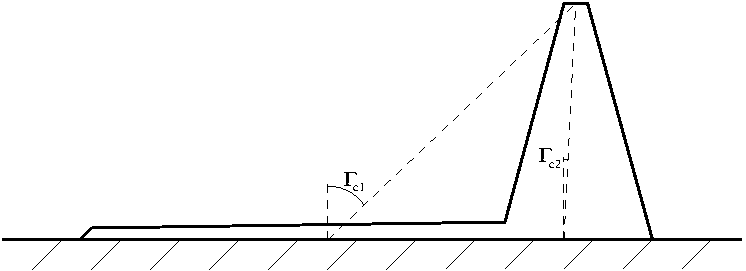
\epsfig{file=figures/fin-geometry/fin-midchord-angle,scale=0.7}
\caption{A free-form fin shape and two possibilities for the midchord
  angle $\Gamma_c$.}
\label{fig-midchord-angle}
\end{figure}

Instead the fin planform is divided into a large number of chords, and
the angle between the midpoints of each two consecutive chords is
calculated.  The midchord angle used in equation~(\ref{eq-CNa1}) is
then the average of all these angles.  This produces an angle better
representing the actual shape of the fin, as angle $\Gamma_{c2}$ in
Figure~\ref{fig-midchord-angle}.  The angle calculated by this method
is also equal to the natural midchord angles for trapezoidal and
elliptical fins.




\subsubsection{Single fin \CNa\ at supersonic speeds}
\label{sec-single-fin-CNa-supersonic}

The method for calculating the normal force coefficient of fins at
supersonic speed presented by Barrowman is based on a third-order
expansion according to Busemann theory~\cite{barrowman-fin}.  The
method divides the fin into narrow streamwise strips, the normal force
of which are calculated separately.  In this presentation the method
is further simplified by assuming the fins to be flat plates and by
ignoring a third-order term that corrects for fin-tip Mach cone
effects.

%
% Angle of Inclination = between ray and surface
% Angle of Incidence   = between ray and normal of surface
%


The local pressure coefficient of strip $i$ is calculated by
%
\begin{equation}
C_{P_i} = K_1 \,\eta_i + K_2 \,\eta_i^2 + K_3 \,\eta_i^3
\label{eq-local-pressure-coefficient}
\end{equation}
%
where $\eta_i$ is the inclination of the flow at the surface and the
coefficients are
%
\begin{align}
K_1 &= \frac{2}{\beta} \\
K_2 &= \frac{(\gamma+1)M^4 - 4\,\beta^2}{4\,\beta^4} \\
K_3 &= \frac{(\gamma+1)M^8 + (2\gamma^2-7\gamma-5)M^6 +
  10(\gamma+1)M^4 + 8}{6\,\beta^7}
\end{align}
%
It is noteworthy that the coefficients $K_1$, $K_2$ and $K_3$ can be
pre-calculated for various Mach numbers, which makes the pressure
coefficient of a single strip very fast to compute.  At small
angles of inclination the pressure coefficient is nearly linear, as
presented in Figure~\ref{fig-fin-strip-pressure-coefficient}.


\begin{figure}
\centering
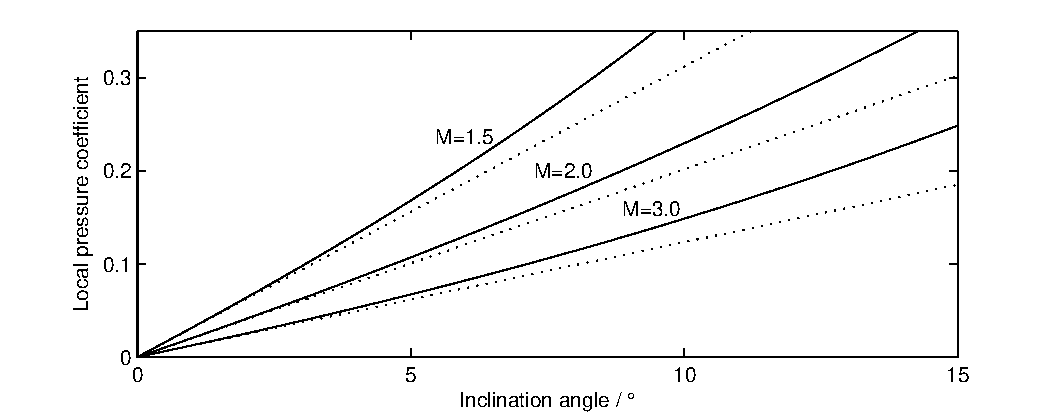
\epsfig{file=figures/fin-geometry/Cp-supersonic,scale=0.6}
\caption{The local pressure coefficient as a function of the
  strip inclination angle at various Mach numbers.  The dotted line
  depicts the linear component of
  equation~(\ref{eq-local-pressure-coefficient}).}
\label{fig-fin-strip-pressure-coefficient}
\end{figure}


%If the rocket is not rolling, the inclinations $\eta_i$ are the
%same for all strips of a fin and only one pressure coefficient needs
%to be computed.  However, presence of a roll velocity generates
%varying inclinations for all strips.  Therefore the current
%examination is performed with separate inclinations and later
%simplified for non-rolling conditions.  The effects of roll are
%further discussed in Section~\ref{sec-roll-dynamics}.

The lift force of strip $i$ is equal to
%
\begin{equation}
F_i = C_{P_i} \cdot \frac{1}{2} \rho v_0^2 \cdot 
  \underbrace{c_i \Delta y}_{\rm area}.
\label{eq-supersonic-strip-lift-force}
\end{equation}
%
The total lift force of the fin is obtained by summing up the
contributions of all fin strips.  The normal force coefficient is then
calculated in the usual manner as
%
\begin{align}
C_N &= \frac{\sum_i F_i}{\frac{1}{2}\rho v_0^2\; \Aref} \\
    &= \frac{1}{\Aref}\sum_i C_{P_i} \cdot c_i\Delta y.
\end{align}

When computing the corrective normal force coefficient of the fins the
effect of roll is not taken into account.  In this case, and
assuming that the fins are flat plates, the inclination angles
$\eta_i$ of all strips are the same, and the pressure coefficient is
constant over the entire fin.  Therefore the normal force coefficient
is simply
%
\begin{equation}
(C_N)_1 = \frac{\Afin}{\Aref} \;C_P.
\end{equation}
%
Since the pressure coefficient is not linear with the angle of attack,
the normal force coefficient slope is defined using
equation~(\ref{eq-CNa-definition}) as
%
\begin{equation}
(\CNa)_1 = \frac{(C_N)_1}{\alpha} = 
 \frac{\Afin}{\Aref} \; \del{K_1 + K_2\,\alpha + K_3\,\alpha^2}.
\end{equation}




\subsubsection{Multiple fin \CNa}
\label{update-roll-angle}

In his thesis, Barrowman considered only configurations with three and
four fins, one of which was parallel to the lateral airflow.  For
simulation purposes, it is necessary to lift these restrictions to
allow for any direction of lateral airflow and for any number of
fins.

The lift force of a fin is perpendicular to the fin and originates
from its CP.  Therefore a single fin may cause a rolling and yawing
moment in addition to a pitching moment.  In this case all of the
forces and moments must be computed from the geometry.  If there are
two or more fins placed symmetrically around the body then the yawing
moments cancel, and if additionally there is no fin cant then the
total rolling moment is also zero, and these moments need not be
computed.

The geometry of an uncanted fin configuration is depicted in
Figure~\ref{fig-dihedral-angle}.  The dihedral angle between each of
the fins and the airflow direction is denoted $\Lambda_i$.  The fin
$i$ encounters a local angle of attack of
%
\begin{equation}
\alpha_i = \alpha \sin\Lambda_i
\end{equation}
%
for which the normal force component (the component parallel to the
lateral airflow) is then
%
\begin{equation}
\del{\CNa}_{\Lambda_i} = \del{\CNa}_1 \sin^2 \Lambda_i.
\end{equation}


\begin{figure}
\centering
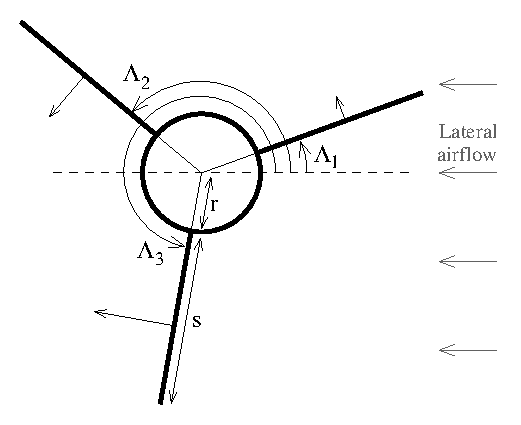
\epsfig{file=figures/fin-geometry/dihedral-angle,scale=1}
\caption{The geometry of an uncanted three-fin configuration (viewed
  from rear).}
\label{fig-dihedral-angle}
\end{figure}


The sum of the coefficients for $N$ fins then yields
%
\begin{equation}
\sum_{k=1}^N \del{\CNa}_{\Lambda_k} =
    \del{\CNa}_1 \sum_{k=1}^N \sin^2\Lambda_k.
\label{N-fin-equation}
\end{equation}
%
However, when $N\geq 3$ and the fins are spaced equally around the
body of the rocket, the sum simplifies to a constant
%
\begin{equation}
\sum_{k=1}^N \sin^2 (2\pi k/N + \theta) = \frac{N}{2}.
\label{N-fin-simplification}
\end{equation}
%
This equation predicts that the normal force produced by three or more
fins is independent of the roll angle $\theta$ of the vehicle.
Investigation by Pettis~\cite{pettis} showed that the normal force
coefficient derivative of a four-finned rocket at Mach~1.48 decreased
by approximately 6\% at a roll angle of $45^\circ$, and the roll angle
had negligible effect on an eight-finned rocket.  Experimental data of
a four-finned sounding rocket at Mach speeds from 0.60 to 1.20
supports the 6\% estimate~\cite{experimental-transonic}.  

The only experimental data available to the author of three-fin
configurations was of a rocket with a rounded triangular body cross
section~\cite{triform-fin-data}.  This data suggests an effect of
approximately 15\% on the normal force coefficient derivative
depending on the roll angle.  However, it is unknown how much of this
effect is due to the triangular body shape and how much from the fin
positioning.

It is also hard to predict such an effect when examining singular
fins.  If three identical or very similar singular fins are placed on
a rocket body, the effect should be the same as when the fins belong
to the same three-fin configuration.  Due to these facts the effect of
the roll angle on the normal force coefficient derivative is ignored
when a fin configuration has three or more fins.
%
\footnote{In OpenRocket versions prior to 0.9.6 a sinusoidal reduction
of 15\% and 6\% was applied to three- and four-fin configurations,
respectively.  However, this sometimes caused a significantly
different predicted CP location compared to the pure Barrowman method,
and also caused a discrepancy when such a fin configuration was
decomposed into singular fins.  It was deemed better to follow the
tested and tried Barrowman method instead of introducing additional
terms to the equation.}

However, in configurations with many fins the fin--fin
interference may cause the normal force to be less than that estimated
directly by equation~(\ref{N-fin-equation}).  According to
reference~\cite[p.~5-24]{MIL-HDBK}, the normal force coefficients
for six and eight-fin configurations are 1.37 and 1.62 times that of
the corresponding four-fin configuration, respectively.  The values
for five and seven-fin configurations are interpolated between these
values.

\pagebreak[4]
Altogether, the normal force coefficient derivative $(\CNa)_N$ is
calculated by:
%
\begin{equation}
(\CNa)_N = \del{\sum_{k=1}^N \sin^2\Lambda_k} \del{\CNa}_1 \cdot
  \left\{ 
\begin{array}{ll}
  1.000\; & N_{\rm tot}=1,2,3,4  \vspace{1mm}\\
  0.948\; & N_{\rm tot}=5  \vspace{1mm}\\
  0.913\; & N_{\rm tot}=6  \vspace{1mm}\\
  0.854\; & N_{\rm tot}=7  \vspace{1mm}\\
  0.810\; & N_{\rm tot}=8  \vspace{1mm}\\
  0.750\; & N_{\rm tot}>8
\end{array}
  \right.
\end{equation}
%
%\begin{equation}
%(\CNa)_N =
%  \left\{ 
%\begin{array}{ll}
%  \del{\sum_{k=1}^N \sin^2\Lambda_k} \del{\CNa}_1 & N=1,2 \vspace{1mm}\\
%  1.50\; \del{\CNa}_1 & N=3  \vspace{1mm}\\
%  2.00\; \del{\CNa}_1 & N=4  \vspace{1mm}\\
%  2.37\; \del{\CNa}_1 & N=5  \vspace{1mm}\\
%  2.74\; \del{\CNa}_1 & N=6  \vspace{1mm}\\
%  2.99\; \del{\CNa}_1 & N=7  \vspace{1mm}\\
%  3.24\; \del{\CNa}_1 & N=8
%\end{array}
%  \right.
%\end{equation}
%
Here $N$ is the number of fins in this fin set, while $N_{\rm tot}$ is
the total number of parallel fins that have an interference effect.
The sum term simplifies to $N/2$ for $N\geq3$ according to
equation~(\ref{N-fin-simplification}).  The interference effect for
$N_{\rm tot}>8$ is assumed at 25\%, as data for such configurations is
not available and such configurations are rare and eccentric in any
case.

\subsubsection{Fin--body interference}

The normal force coefficient must still be corrected for fin--body
interference, which increases the overall produced normal force.  Here
two distinct effects can be identified: the normal force on the fins
due to the presence of the body and the normal force on the body due
to the presence of fins.  Of these the former is significantly larger;
the latter is therefore ignored.  The effect of the extra fin lift is
taken into account using a correction term
%
\begin{equation}
\del{\CNa}_{T(B)} = K_{T(B)}\;\del{\CNa}_N
\end{equation}
%
where $\del{\CNa}_{T(B)}$ is the normal force coefficient derivative
of the tail in the presence of the body.  The term $K_{T(B)}$ can be
approximated by~\cite{barrowman-rd}
%
\begin{equation}
K_{T(B)} = 1 + \frac{r_t}{s + r_t},
\end{equation}
%
where $s$ is the fin span from root to tip and $r_t$ is the body
radius at the fin position.  The value $\del{\CNa}_{T(B)}$ is then
used as the final normal force coefficient derivative of the fins.


%The normal force coefficient must still be corrected for fin--body
%interference, which increases the produced normal force.  The effect
%of the interference can be split into two components, the normal force
%of the fins in the presence of the body $\del{\CNa}_{T(B)}$ and of the
%body in the presence of the fins $\del{\CNa}_{B(T)}$.  (The subscript
%$T$ refers to {\it tail}.)  The interference is taken into account
%using the correction factors
%%
%\begin{align}
%\del{\CNa}_{T(B)} &= K_{T(B)}\;\del{\CNa}_N \\
%\del{\CNa}_{B(T)} &= K_{B(T)}\;\del{\CNa}_N.
%\end{align}
%%
%In his original report, Barrowman simplified the factor $K_{T(B)}$ to
%%
%\begin{equation}
%K_{T(B)} = 1 + \frac{r_t}{s + r_t},
%\end{equation}
%%
%where $s$ is the fin span from root to tip and $r_t$ is the body
%radius at the fin position, and ignored the effect of $K_{B(T)}$ as
%small compared to $K_{T(B)}$ for typical fin dimensions.  However,
%$K_{T(B)}$ may be significant for fins with a span short compared to
%the body radius.  In his thesis, a more accurate equation for
%$K_{T(B)}$ is provided, and $K_{B(T)}$ is given
%as~\cite[p.~31]{barrowman-thesis}
%%
%\begin{equation}
%K_{B(T)} = \del{1 + \frac{r_t}{s + r_t}}^2 - K_{T(B)}.
%\end{equation}
%%
%Therefore the total interference effect can be accounted for by a
%factor
%%
%\begin{equation}
%K_T = K_{T(B)} + K_{B(T)} = \del{1 + \frac{r_t}{s + r_t}}^2
%\end{equation}
%%
%and
%%
%\begin{equation}
%\del{\CNa}_{\rm fins} = K_T\; (\CNa)_N.
%\end{equation}

%This equation takes the increase on body lift and adds it as an
%additional force on the fins.  The equation holds at subsonic speeds
%and also at supersonic speeds until the fin tip Mach cone intersects
%the body.  In the latter case more complex interference factors would
%be required, which have been ignored in the current software.

% TODO: FUTURE: supersonic interference effects, MIL-HDBK page 5-25 or B'man



\pagebreak[4]
\subsection{Pitch damping moment}

So far the effect of the current pitch angular velocity has been
ignored as marginal.  This is the case during the upward flight of a
stable rocket.  However, if a rocket is launched nearly vertically in
still air, the rocket flips over rather rapidly at apogee.  In
some cases it was observed that the rocket was left wildly oscillating
during descent.  The pitch damping moment opposes the fast rotation of
the rocket thus damping the oscillation.

Since the pitch damping moment is notable only at apogee, and
therefore does not contribute to the overall flight characteristics,
only a rough estimate of its magnitude is required.  A cylinder in
perpendicular flow has a drag coefficient of approximately $C_D=1.1$,
with the reference area being the planform area of the
cylinder~\cite[p.~3-11]{hoerner}.  Therefore a short piece of cylinder
$\dif\xi$ at a distance $\xi$ from a rotation axis, as shown in
Figure~\ref{fig-pitch-velocity}, produces a force
%
\begin{equation}
\dif F = 1.1 \cdot \frac{1}{2}\rho(\omega\xi)^2 \cdot 
\underbrace{2r_t\,\dif\xi}_{\rm ref.area}
\end{equation}
%
when the cylinder is rotating at an angular velocity $\omega$.  The
produced moment is correspondingly $\dif m = \xi\dif F$.  Integrating
this over $0\ldots l$ yields the total pitch moment
%
\begin{equation}
m = 0.275 \cdot \rho\, r_t\, l^4 \omega^2
\end{equation}
%
and thus the moment damping coefficient is
%
\begin{equation}
C_{\rm damp} = 
    0.55 \cdot \frac{l^4\; r_t}{\Aref\, d}\cdot\frac{\omega^2}{v_0^2}.
\end{equation}
%
This value is computed separately for the portions of the rocket body
fore and aft of the CG using an average body radius as $r_t$.

\begin{figure}
\centering
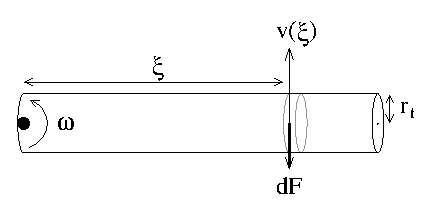
\epsfig{file=figures/components/body-pitch-rate,scale=0.8}
\caption{Pitch damping moment due to a pitching body component.}
\label{fig-pitch-velocity}
\end{figure}



Similarly, a fin with area $\Afin$ at a distance $\xi$ from the CG
produces a moment of approximately
%
\begin{equation}
C_{\rm damp} = 
    0.6\cdot \frac{N\,\Afin\;\xi^3}{\Aref\,d}\cdot\frac{\omega^2}{v_0^2}
\end{equation}
%
where the effective area of the fins is assumed to be 
$\Afin\cdot N/2$.  For $N>4$ the value $N=4$ is used, since the other
fins are not exposed to any direct airflow.

The damping moments are applied to the total pitch moment in the
opposite direction of the current pitch rate.  It is noteworthy
that the damping moment coefficients are proportional to $\omega^2/v_0^2$,
confirming that the damping moments are insignificant during most of
the rocket flight, where the angles of deflection are small and the
velocity of the rocket large.  Through roll coupling the yaw rate may also
momentarily become significant, and therefore the same correction is
also applied to the yaw moment.





\clearpage
\section{Roll dynamics}
\label{sec-roll-dynamics}

When the fins of a rocket are canted at some angle $\delta>0$, the
fins induce a rolling moment on the rocket.  On the other hand, when a
rocket has a specific roll velocity, the portions of the fin far from
the rocket centerline encounter notable tangential velocities
which oppose the roll.  Therefore a steady-state roll velocity,
dependent on the current velocity of the rocket, will result.

The effect of roll on a fin can be examined by dividing the fin into
narrow streamwise strips and later integrating over the strips.  A
strip $i$ at distance $\xi_i$ from the rocket centerline encounters a
radial velocity
%
\begin{equation}
u_i = \omega \xi_i
\end{equation}
%
where $\omega$ is the angular roll velocity, as shown in
Figure~\ref{fig-roll-velocity}.  The radial velocity induces an angle
of attack
%
\begin{equation}
\eta_i = \tan^{-1} \del{\frac{u_i}{v_0}} =
\tan^{-1}\del{\frac{\omega\xi_i}{v_0}}
\approx \frac{\omega\xi_i}{v_0}
\label{eq-tan-approx}
\end{equation}
%
to the strip.  The approximation $\tan^{-1} \eta \approx \eta$ is
valid for $u_i\ll v_0$, that is, when the velocity of the rocket is
large compared to the radial velocity.  The approximation is
reasonable up to angles of $\eta \approx 20^\circ$, above which angle
most fins stall, which limits the validity of the equation in any
case.  

When a fin is canted at an angle $\delta$, the total
inclination of the strip to the airflow is
%
\begin{equation}
\alpha_i = \delta - \eta_i.
\label{eq-roll-aoa-variation}
\end{equation}

Assuming that the force produced by a strip is directly proportional
to the local angle of attack, the force on strip $i$ is
%
\begin{equation}
F_i = k_i \alpha_i = k_i (\delta - \eta_i)
\end{equation}
%
for some $k_i$.  The total moment produced by the fin is then
%
\begin{equation}
%l = \int_0^s (r+y) k (\delta-\eta(y))\dif y
%  = \int_0^s (r+y) k \delta \dif y - \int_0^s (r+y) k \eta(y) \dif y
l = \sum_i \xi_i F_i = \sum_i \xi_i k_i (\delta - \eta_i)
  = \sum_i \xi_i k_i \delta - \sum_i \xi_i k_i \eta_i.
\end{equation}
%
This shows that the effect of roll can be split into two components:
the first term $\sum_i \xi_i k_i \delta$ is the roll moment induced by
a fin canted at the angle $\delta$ when flying at zero roll rate
($\omega=0$), while the second term $\sum_i \xi_i k_i \eta_i$ is the
opposing moment generated by an uncanted fin ($\delta=0$) when flying
at a roll rate $\omega$.  These two moments are called the roll
forcing moment and roll damping moment, respectively.  These
components will be analyzed separately.


\begin{figure}
\centering
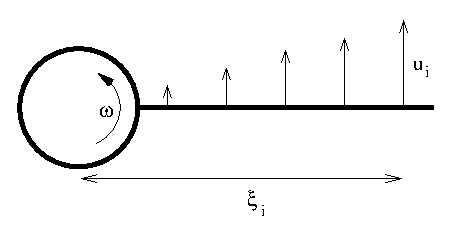
\epsfig{file=figures/fin-geometry/roll-velocity,scale=0.8}
\caption{Radial velocity at different positions of a fin.  Viewed from
  the rear of the rocket.}
\label{fig-roll-velocity}
\end{figure}



\subsection{Roll forcing coefficient}

As shown previously, the roll forcing coefficient can be computed by
examining a rocket with fins canted at an angle $\delta$ flying at
zero roll rate ($\omega=0$).  In this case, the cant angle $\delta$ acts
simply as an angle of attack for each of the fins.  Therefore, the
methods computed in the previous section can be directly applied.
Because the lift force of a fin originates from the mean aerodynamic
chord, the roll forcing coefficient of $N$ fins is equal to
%
\begin{equation}
C_{lf} = \frac{N (y_{\rm MAC}+r_t) \del{\CNa}_1 \delta}{d}
\label{eq-roll-forcing-moment}
\end{equation}
%
where $y_{\rm MAC}$ and $\del{\CNa}_1$ are computed using the methods
described in Section~\ref{sec-planar-fins} and $r_t$ is the radius of
the body tube at the fin position.  This result is applicable
for both subsonic and supersonic speeds.



\subsection{Roll damping coefficient}

The roll damping coefficient is computed by examining a rocket with
uncanted fins ($\delta=0$) flying at a roll rate $\omega$.  Since
different portions of the fin encounter different local angles of
attack, the damping moment must be computed from the separate
streamwise airfoil strips.

At subsonic speeds the force generated by strip $i$ is equal to
%
\begin{equation}
F_i = \CNa_0 \; \frac{1}{2}\rho v_0^2 \; 
\underbrace{c_i \Delta\xi_i}_{\rm area} \; \eta_i.
\end{equation}
%
Here $\CNa_0$ is calculated by equation~(\ref{eq-fin-CNa0}) and 
$c_i \Delta\xi_i$ is the area of the strip.  The roll damping moment
generated by the strip is then
%
\begin{equation}
\del{C_{ld}}_i
  = \frac{F_i\,\xi_i}{\frac{1}{2}\rho v_0^2\,\Aref\, d}
  = \frac{\CNa_0}{\Aref\,d} \; \xi_i c_i\Delta\xi_i \; \eta_i.
\end{equation}
%
By applying the approximation~(\ref{eq-tan-approx}) and summing
(integrating) the airfoil strips the total roll damping moment for $N$
fins is obtained as:
%
\begin{align}
C_{ld} & = N \sum_i (C_{ld})_i \nonumber \\
& = \frac{N \;\CNa_0\;\omega}{\Aref\,d\,v_0} \sum_i c_i\xi_i^2\Delta\xi_i.
\label{eq-roll-damping-moment}
\end{align}
%
The sum term is a constant for a specific fin shape.  It can be
computed numerically from the strips or analytically for specific
shapes.  For trapezoidal fins the term can be integrated as
%
\begin{equation}
\sum_i c_i\xi_i^2\Delta\xi_i = 
\frac{C_r+C_t}{2}\;r_t^2s + \frac{C_r+2C_t}{3}\;r_ts^2 + 
\frac{C_r+3C_t}{12}\;s^3
\end{equation}
%
and for elliptical fins
%
\begin{equation}
\sum_i c_i\xi_i^2\Delta\xi_i = 
C_r \del{ \frac{\pi}{4}\;r_t^2s + \frac{2}{3}\;r_ts^2 +
  \frac{\pi}{16}\;s^3 }.
\end{equation}


The roll damping moment at supersonic speeds is calculated
analogously, starting from the supersonic strip lift force,
equation~(\ref{eq-supersonic-strip-lift-force}), where the angle of
inclination of each strip is calculated using
equation~(\ref{eq-tan-approx}).  The roll moment at supersonic speeds
is thus
%
\begin{equation}
C_{ld} = \frac{N}{\Aref\,d} \sum_i C_{P_i}\, c_i \xi_i \Delta \xi_i.
\end{equation}
%
The dependence on the incidence angle $\eta_i$ is embedded within the
local pressure coefficient $C_{P_i}$,
equation~(\ref{eq-local-pressure-coefficient}).  Since the dependence
is non-linear, the sum term is a function of the Mach number as well
as the fin shape.




\subsection{Equilibrium roll frequency}

One quantity of interest when examining rockets with canted fins
is the steady-state roll frequency that the fins induce on a rocket
flying at a specific velocity.  This is obtained by equating the roll
forcing moment~(\ref{eq-roll-forcing-moment}) and roll damping
moment~(\ref{eq-roll-damping-moment}) and solving for the roll rate
$\omega$.  The equilibrium roll frequency at subsonic speeds is
therefore
%
\begin{equation}
f_{\rm eq} = \frac{\omega_{\rm eq}}{2\pi} =
\frac{\Aref\; \beta v_0 \; y_{\rm MAC} \; (\CNa)_1 \; \delta}
{4\pi^2\; \sum_i c_i\xi_i^2\Delta\xi_i}
\label{eq-subsonic-roll-rate}
\end{equation}
%
It is worth noting that the arbitrary reference area \Aref\ is
cancelled out by the reference area appearing within $(\CNa)_1$,
as is to be expected.

At supersonic speeds the dependence on the incidence angle is
non-linear and therefore the equilibrium roll frequency must be solved
numerically.  Alternatively, the second and third-order terms of the
local pressure coefficient of
equation~(\ref{eq-local-pressure-coefficient}) may be ignored, in
which case an approximation for the equilibrium roll frequency nearly
identical to the subsonic case is obtained:
%
\begin{equation}
f_{\rm eq} = \frac{\omega_{\rm eq}}{2\pi} =
\frac{\Aref\; \beta v_0 \; y_{\rm MAC} \; (\CNa)_1 \; \delta}
{4\pi\; \sum_i c_i\xi_i^2\Delta\xi_i}
\label{eq-supersonic-roll-rate}
\end{equation}
%
The value of $(\CNa)_1$ must, of course, be computed using different
methods in the subsonic and supersonic cases.




%\subsection{Roll sensitivity}
%
%The vast majority of model rockets have uncanted fins and in
%principle no roll is induced to these rockets.  However, in practice
%imprecision in the attachment of the fins and other protrusions always
%cause some roll to the rocket during flight.  In some applications,
%such as launching rockets with onboard video cameras, it is desirable
%to design the rockets so as to minimize the roll rate.  To assist this
%design, a quantity called the {\it roll sensitivity} of the rocket is
%defined as
%%
%\begin{equation}
%f_{\rm sens} = \frac{1}{N}\eval{\pd{f_{\rm eq}}{\delta}}_{\delta=0}.
%\end{equation}
%%
%This is the slope of the equilibrium roll frequency at $\delta=0$,
%divided by the number of fins.  If measured in units of 
%$\rm Hz/^\circ$, the quantity indicates the number of rotations per
%second induced by one fin being attached at an angle of $1^\circ$.  By
%minimizing the roll sensitivity of a rocket, the effect of
%construction imperfections on the roll rate can be minimized.  From
%equation~(\ref{eq-roll-rate}) the subsonic roll sensitivity is
%obtained as
%%
%\begin{equation}
%f_{\rm sens} =
%\frac{\Aref\; \beta v_0 \; y_{\rm MAC} \; (\CNa)_1}
%{N\; 4\pi^2\; \sum_i c_i\xi_i^2\Delta\xi_i}
%\end{equation}
%%
%or conversely,
%%
%\begin{equation}
%f_{\rm eq} = N\; f_{\rm sens}\,\delta.
%\end{equation}
%%
%Similarly, in supersonic flight the roll sensitivity may either be
%solved numerically, or computed using the linear approximation for
%$C_{P_i}$ yielding 
%%
%\begin{equation}
%f_{\rm sens} = 
%\frac{\Aref\; \beta v_0 \; y_{\rm MAC} \; (\CNa)_1}
%{N\; 4\pi\; \sum_i c_i\xi_i^2\Delta\xi_i}.
%\end{equation}
%
%
%When the fins are canted by design, the roll sensitivity loses its
%significance.  Therefore if all the fins on a rocket are uncanted, the
%quantity of intrest is the roll sensitivity, while for a rocket with
%canted fins it is the equilibrium roll frequency.






\clearpage
\section{Drag forces}
\label{sec-drag}

Air flowing around a solid body causes drag, which resists the
movement of the object relative to the air.  Drag forces arise from
two basic mechanisms, the air pressure distribution around the rocket
and skin friction.  The pressure distribution is further divided into
body pressure drag (including shock waves generated as supersonic
speeds), parasitic pressure drag due to protrusions such as launch
lugs and base drag.  Additional sources of drag include interference
between the fins and body and vortices generated at fin tips when
flying at an angle of attack.  The different drag sources are depicted
in Figure~\ref{fig-drag-components}.  Each drag source will be analyzed
separately; the interference drag and fin-tip vortices will be
ignored as small compared to the other sources.

As described in Section~\ref{sec-general-aerodynamics}, two different
drag coefficients can be defined: the (total) drag coefficient $C_D$
and the axial drag coefficient $C_A$.  At zero angle of attack these
two coincide, $C_{D_0} = C_{A_0}$, but at other angles a distinction
between the two must be made.  The value of significance in the
simulation is the axial drag coefficient $C_A$ based on the choice of
force components.  However, the drag coefficient $C_D$ describes the
deceleration force on the rocket, and is a more commonly known value
in the rocketry community, so it is informational to calculate its
value as well.

In this section the zero angle-of-attack drag coefficient
$C_{D_0} = C_{A_0}$ will be computed first.  Then, in
Section~\ref{sec-axial-drag} this will be extended for angles of
attack and $C_A$ and $C_D$ will be computed.  Since the drag force of
each component is proportional to its particular size, the subscript
$\bullet$ will be used for coefficients that are computed using the
reference area of the specific component.  This reference area is the
frontal area of the component unless otherwise noted.  Conversion to
the global reference area is performed by
%
\begin{equation}
C_{D_0} = \frac{A_{\rm component}}{\Aref} \cdot C_{D\bullet}.
\end{equation}


\begin{figure}
\centering
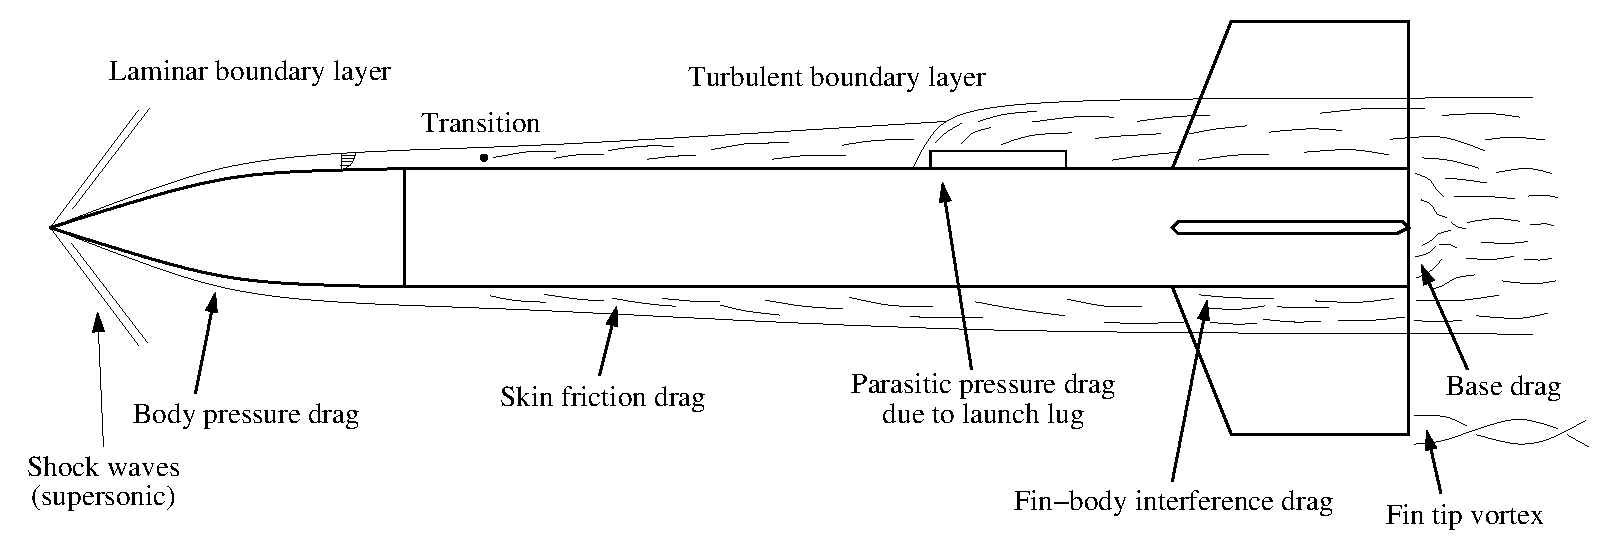
\epsfig{file=figures/aerodynamics/drag-components,width=13.5cm}
\caption{Types of model rocket drag at subsonic speeds.}
\label{fig-drag-components}
\end{figure}


\subsection{Laminar and turbulent boundary layers}

At the front of a streamlined body, air flows smoothly around the
body in layers, each of which has a different velocity.  The layer
closest to the surface ``sticks'' to the object having zero velocity.
Each layer gradually increases the speed until the free-stream
velocity is reached.  This type of flow is said to be {\it laminar}
and to have a {\it laminar boundary layer}.  The thickness of the
boundary layer increases with the distance the air has flowed along
the surface.  At some point a transition occurs and the layers of air
begin to mix.  The boundary layer becomes {\it turbulent} and thickens
rapidly.  This transition is depicted in
Figure~\ref{fig-drag-components}.

A turbulent boundary layer induces a notably larger skin friction drag
than a laminar boundary layer.  It is therefore necessary to consider
how large a portion of a rocket is in laminar flow and at what point
the flow becomes turbulent.  The point at which the flow becomes
turbulent is the point that has a {\it local critical Reynolds number}
%
\begin{equation}
R_{\rm crit} = \frac{v_0 \; x}{\nu},
\label{eq-transition-Re}
\end{equation}
%
where $v_0$ is the free-stream air velocity, $x$ is the distance along
the body from the nose cone tip and 
$\nu\approx 1.5\cdot10^{-5}\;\rm m^2/s$ is the kinematic viscosity of
air.  The critical Reynolds number is approximately 
$R_{\rm crit} = 5\cdot10^5$~\cite[p.~43]{barrowman-thesis}. Therefore,
at a velocity of 100~m/s the transition therefore occurs approximately
7~cm from the nose cone tip.

% Air viscosity:
% http://www.engineeringtoolbox.com/air-absolute-kinematic-viscosity-d_601.html


%Since the drag force is approximately proportional to the square of
%the free-stream velocity, the value of $C_D$ is most critical at high
%velocities.  Equation~(\ref{eq-transition-Re}) shows that at a velocity
%of 100~m/s the transition to turbulent flow occurs about 7~cm
%from the nose cone tip.  Therefore at these speeds most of the wetted
%area of a typical model rocket is in turbulent flow.

Surface roughness or even slight protrusions may also trigger the
transition to occur prematurely.  At a velocity of 60~m/s the critical
height for a cylindrical protrusion all around the body is of the
order of 0.05~mm~\cite[p.~348]{advanced-model-rocketry}.  The
body-to-nosecone joint, a severed paintbrush hair or some other
imperfection on the surface may easily exceed this limit and cause
premature transition to occur.

Barrowman presents methods for computing the drag of both fully
turbulent boundary layers as well as partially-laminar layers.  Both
methods were implemented and tested, but the difference in apogee
altitude was less than 5\% in with all tested designs.  Therefore,
the boundary layer is assumed to be fully turbulent in all cases.

%A typical model rocket may therefore be assumed to have a fully
%turbulent boundary layer.  Only sport models which have been
%finished to fine precision may benefit from a partial laminar
%flow around the rocket.  These different types of rockets will be
%taken into account by having two modes of calculation, one for typical
%model rockets that assumes a fully turbulent boundary layer, and
%another one which assumes very fine precision finish.






\subsection{Skin friction drag}

Skin friction is one of the most notable sources of model rocket
drag.  It is caused by the friction of the viscous flow of air
around the rocket.  In his thesis Barrowman presented formulae for
estimating the skin friction coefficient for both laminar and
turbulent boundary layers as well as the transition between the
two~\cite[pp.~43--47]{barrowman-thesis}.  As discussed above, a fully
turbulent boundary layer will be assumed in this thesis.

The skin friction coefficient $C_f$ is defined as the drag coefficient
due to friction with the reference area being the total wetted area
of the rocket, that is, the body and fin area in contact with the
airflow:
%
\begin{equation}
C_f = \frac{D_{\rm friction}}{\frac{1}{2} \rho v_0^2\;A_{\rm wet}}
\end{equation}
%
The coefficient is a function of the rocket's Reynolds number $R$ and
the surface roughness.  The aim is to first calculate the skin
friction coefficient, then apply corrections due to compressibility
and geometry effects, and finally to convert the coefficient to the
proper reference area.


\subsubsection{Skin friction coefficients}
\label{sec-skin-friction-coefficient}

The values for $C_f$ are given by different formulae depending on the
Reynolds number.  For fully turbulent flow the coefficient is given by
%
\begin{equation}
C_f = \frac{1}{(1.50\; \ln R - 5.6)^2}.
\label{eq-turbulent-friction}
\end{equation}

The above formula assumes that the surface is ``smooth'' and the
surface roughness is completely submerged in a thin, laminar sublayer.
At sufficient speeds even slight roughness may have an effect on the
skin friction.  The critical Reynolds number corresponding to the
roughness is given by
%
\begin{equation}
R_{\rm crit} = 51\left(\frac{R_s}{L}\right)^{-1.039},
\end{equation}
%
where $R_s$ is an approximate roughness height of the surface.  A few
typical roughness heights are presented in Table~\ref{tab-roughnesses}.
For Reynolds numbers above the critical value, the skin friction
coefficient can be considered independent of Reynolds number, and has
a value of
%
\begin{equation}
C_f = 0.032\left(\frac{R_s}{L}\right)^{0.2}.
\label{eq-critical-friction}
\end{equation}
%


\begin{table}
\caption{Approximate roughness heights of different
  surfaces~\cite[p.~5-3]{hoerner}}
\label{tab-roughnesses}
\begin{center}
\begin{tabular}{lc}
Type of surface & Height / \um \\
\hline
Average glass                  & 0.1 \\
Finished and polished surface  & 0.5 \\
Optimum paint-sprayed surface  & 5 \\
Planed wooden boards           & 15 \\
% planed = h�yl�tty ???
Paint in aircraft mass production & 20 \\
Smooth cement surface          & 50 \\
Dip-galvanized metal surface   & 150 \\
Incorrectly sprayed aircraft paint & 200 \\
Raw wooden boards              & 500 \\
Average concrete surface       & 1000 \\
\hline
\end{tabular}
\end{center}
\end{table}


Finally, a correction must be made for very low Reynolds numbers.  The
experimental formulae are applicable above approximately
$R\approx10^4$.  This corresponds to velocities typically below 1~m/s,
which therefore have negligible effect on simulations.  Below this
Reynolds number, the skin friction coefficient is assumed to be equal
as for $R=10^4$.

Altogether, the skin friction coefficient for turbulent flow is
calculated by
%
\begin{equation}
C_f = \left\{
\begin{array}{ll}
1.48\cdot10^{-2}, & \mbox{if $R<10^4$} \\
\mbox{Eq.~(\ref{eq-turbulent-friction})}, & \mbox{if $10^4<R<R_{\rm crit}$} \\
\mbox{Eq.~(\ref{eq-critical-friction})}, & \mbox{if $R>R_{\rm crit}$}
\end{array}
\right. .
\end{equation}
%
These formulae are plotted with a few different surface roughnesses in
Figure~\ref{fig-skinfriction-plot}.  Included also is the laminar and
transitional skin friction values for comparison.

\begin{figure}
\centering
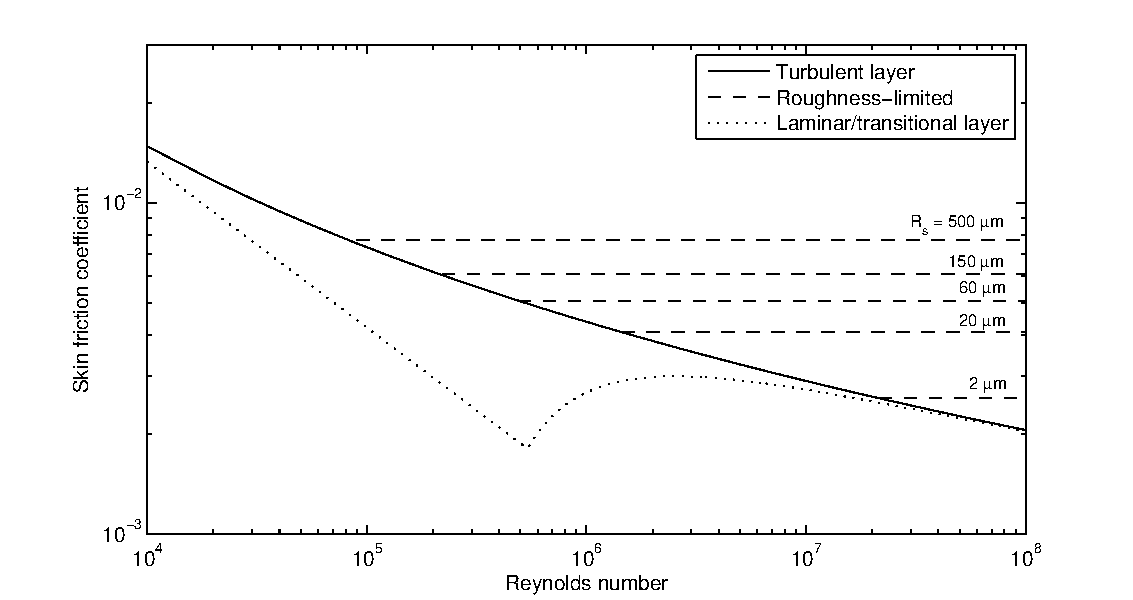
\epsfig{file=figures/drag/skin-friction-coefficient,width=11cm}
\caption{Skin friction coefficient of turbulent, laminar and
  roughness-limited boundary layers.}
\label{fig-skinfriction-plot}
\end{figure}


\subsubsection{Compressibility corrections}

A subsonic speeds the skin friction coefficient turbulent and
roughness-limited boundary layers need to be corrected for
compressibility with the factor
%
\begin{equation}
{C_f}_c = C_f\; (1-0.1\, M^2).
\end{equation}
%
In supersonic flow, the turbulent skin friction coefficient must be
corrected with
%
\begin{equation}
{C_f}_c = \frac{C_f}{(1+0.15\, M^2)^{0.58}}
\end{equation}
%
and the roughness-limited value with
%
\begin{equation}
{C_f}_c = \frac{C_f}{1 + 0.18\, M^2}.
\end{equation}
%
However, the corrected roughness-limited value should not be used if
it would yield a value smaller than the corresponding turbulent
value.


\subsubsection{Skin friction drag coefficient}
\label{sec-skin-friction-drag}

After correcting the skin friction coefficient for compressibility
effects, the coefficient can be converted into the actual drag
coefficient.  This is performed by scaling it to the correct reference
area.  The body wetted area is corrected for its cylindrical geometry,
and the fins for their finite thickness.
%effect of finite fin thickness which Barrowman handled
%separately is also included~\cite[p.~55]{barrowman-thesis}.  
The total friction drag coefficient is then
%
\begin{equation}
(C_D)_{\rm friction} = {C_f}_c \; \frac{
  \del{1 + \frac{1}{2f_B}} \cdot A_{\rm wet,body} + 
  \del{1 + \frac{2t}{\bar c}} \cdot A_{\rm wet,fins}}
   {\Aref}
\label{eq-friction-drag-scale}
\end{equation}
%
where $f_B$ is the fineness ratio of the rocket, and $t$ the thickness
and $\bar c$ the mean aerodynamic chord length of the fins.  The
wetted area of the fins $A_{\rm wet,fins}$ includes both sides of the
fins.





\subsection{Body pressure drag}

Pressure drag is caused by the air being forced around the rocket.  A
special case of pressure drag are shock waves generated at supersonic
speeds.  In this section methods for estimating the pressure drag of
nose cones will be presented and reasonable estimates also for
shoulders and boattails.


\subsubsection{Nose cone pressure drag}

At subsonic speeds the pressure drag of streamlined nose cones is
significantly smaller than the skin friction drag.  In fact, suitable
shapes may even yield negative pressure drag coefficients, producing a
slight reduction in drag.  Figure~\ref{fig-nosecone-cd} presents
various nose cone shapes and their respective measured pressure drag
coefficients.~\cite[p.~3-12]{hoerner}

It is notable that even a slight rounding at the joint between the nose
cone and body reduces the drag coefficient dramatically.  Rounding the
edges of an otherwise flat head reduces the drag coefficient from 0.8
to 0.2, while a spherical nose cone has a coefficient of only 0.01.
The only cases where an appreciable pressure drag is present is when
the joint between the nose cone and body is not smooth, which may
cause slight flow separation.

The nose pressure drag is approximately
proportional to the square of the sine of the joint angle $\phi$
(shown in
Figure~\ref{fig-nosecone-cd})~\cite[p.~237]{handbook-supersonic-aerodynamics}:
%
\begin{equation}
(C_{D\bullet,M=0})_p = 0.8 \cdot \sin^2\phi.
\label{eq-nosecone-pressure-drag}
\end{equation}
%
This yields a zero pressure drag for all nose cone shapes that have a
smooth transition to the body.  The equation does not take into
account the effect of extremely blunt nose cones (length less than
half of the diameter).  Since the main drag cause is slight flow
separation, the coefficient cannot be corrected for compressibility
effects using the Prandtl coefficient, and the value is applicable
only at low subsonic velocities.

\begin{figure}
\centering
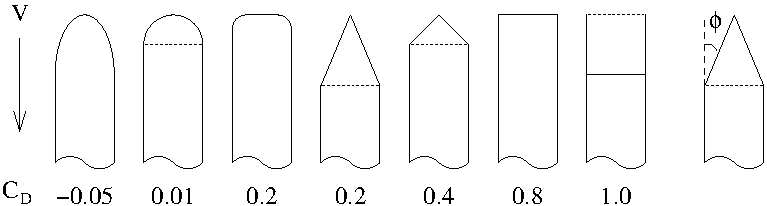
\epsfig{file=figures/nose-geometry/nosecone-cd-top,width=11cm}
\caption{Pressure drag of various nose cone
  shapes~\cite[p.~3-12]{hoerner}.}
\label{fig-nosecone-cd}
\end{figure}


At supersonic velocities shock waves increase the pressure drag
dramatically. In his report Barrowman uses a second-order
shock-expansion method that allows determining the pressure
distribution along an arbitrary slender rotationally symmetrical
body~\cite{second-order-shock-expansion-method}.  However,
the method has some problematic limitations.  The method cannot handle
body areas that have a slope larger than approximately $30^\circ$,
present in several typical nose cone shapes.  The local airflow in
such areas may decrease below the speed of sound, and the method
cannot handle transonic effects.  Drag in the transonic
region is of special interest for rocketeers wishing to build rockets
capable of penetrating the sound barrier.

Instead of a general piecewise computation of the air pressure around
the nose cone, a simpler semi-empirical method for estimating the
transonic and supersonic pressure drag of nose cones is used.  The
method, described in detail in
Appendix~\ref{app-nosecone-drag-method}, combines theoretical and
empirical data of different nose cone shapes to allow estimating the
pressure drag of all the nose cone shapes described in
Appendix~\ref{app-nosecone-geometry}.

The semi-empirical method is used at Mach numbers above 0.8.  
At high subsonic velocities the pressure drag is interpolated between
that predicted by equation~(\ref{eq-nosecone-pressure-drag}) and the
transonic method.  The pressure drag is assumed to be non-decreasing
in the subsonic region and to have zero derivative at $M=0$.  A
suitable interpolation function that resembles the shape of the
Prandtl factor is
%
\begin{equation}
(C_{D\bullet})_{\rm pressure} = a\cdot M^b + (C_{D\bullet,M=0})_p
\label{eq-nosecone-pressure-interpolator}
\end{equation}
%
where $a$ and $b$ are computed to fit the drag coefficient and its
derivative at the lower bound of the transonic method.



\subsubsection{Shoulder pressure drag}

Neither Barrowman nor Hoerner present theoretical or experimental
data on the pressure drag of transitions at subsonic velocities.  In
the case of shoulders, the pressure drag coefficient is assumed to be
the same as that of a nose cone, except that the reference area is the
difference between the aft and fore ends of the transition.  The
effect of a non-smooth transition at the beginning of the shoulder is
ignored, since this causes an increase in pressure and thus cannot
cause flow separation.

While this assumption is reasonable at subsonic velocities, it is
somewhat dubious at supersonic velocities.  However, no comprehensive
data set of shoulder pressure drag at supersonic velocities was
found.  Therefore the same assumption is made for supersonic
velocities and a warning is generated during such simulations (see
Section~\ref{sec-warnings}).  The refinement of the supersonic
shoulder pressure drag estimation is left as a future enhancement.



\subsubsection{Boattail pressure drag}

The estimate for boattail pressure drag is based on the body base
drag estimate, which will be presented in Section~\ref{sec-base-drag}.
At one extreme, the transition length is zero, in which case the
boattail pressure drag will be equal to the total base drag.  On the
other hand, a gentle slope will allow a gradual pressure change
causing approximately zero pressure drag.  Hoerner has presented
pressure drag data for wedges, which suggests that at a
length-to-height ratio below 1 has a constant pressure drag
corresponding to the base drag and above a ratio of 3 the pressure
drag is negligible.  Based on this and the base drag
equation~(\ref{eq-base-drag}), an approximation for the pressure drag
of a boattail is given as
%
\begin{equation}
(C_{D\bullet})_{\rm pressure} =
\frac{A_{\rm base}}{A_{\rm boattail}} \cdot (C_{D\bullet})_{\rm base}
\cdot 
\left\{
\begin{array}{cl}
1 & \mbox{if\ } \gamma < 1 \\
\frac{3-\gamma}{2} & \mbox{if\ } 1 < \gamma < 3 \\
0 & \mbox{if\ } \gamma > 3
\end{array}
\right.
\end{equation}
%
where the length-to-height ratio $\gamma = l/(d_1-d_2)$ is calculated
from the length and fore and aft diameters of the boattail.  The
ratios 1 and 3 correspond to reduction angles of $27^\circ$ and
$9^\circ$, respectively, for a conical boattail.  The base drag
$(C_{D\bullet})_{\rm base}$ is calculated using
equation~(\ref{eq-base-drag}).

Again, this approximation is made primarily based on subsonic data.
At supersonic velocities expansion fans exist, the counterpart of
shock waves in expanding flow.  However, the same equation is used for
subsonic and supersonic flow and a warning is generated during
transonic simulation of boattails.



\subsection{Fin pressure drag}

The fin pressure drag is highly dependent on the fin profile shape.
Three typical shapes are considered, a rectangular profile, rounded
leading and trailing edges, and an airfoil shape with rounded leading
edge and tapering trailing edge.  Barrowman estimates the fin pressure
drag by dividing the drag further into components of a finite
thickness leading edge, thick trailing edge and overall fin
thickness~\cite[p.~48--57]{barrowman-thesis}.  In this report the fin
thickness was already taken into account as a correction to the skin
friction drag in Section~\ref{sec-skin-friction-drag}.  The division
to leading and trailing edges also allows simple extension to the
different profile shapes.

The drag of a rounded leading edge can be considered as a circular
cylinder in cross flow with no base drag.  Barrowman derived 
an empirical formula for the leading edge pressure drag as
%
\begin{equation}
(C_{D\bullet})_{LE\perp} = 
\left\{ 
\begin{array}{ll}
  (1-M^2)^{-0.417} - 1 & \mbox{for $M<0.9$} \\
  1-1.785(M-0.9)         & \mbox{for $0.9 < M < 1$} \\
  1.214 - \frac{0.502}{M^2} + \frac{0.1095}{M^4} & \mbox{for $M>1$}
\end{array}
  \right. .
\end{equation}
%
The subscript $\perp$ signifies the the flow is perpendicular to the
leading edge.

In the case of a rectangular fin profile the leading edge pressure
drag is equal to the stagnation pressure drag as derived in 
equation~\ref{eq-blunt-cylinder-drag} of
Appendix~\ref{app-blunt-cylinder-drag}:
\begin{equation}
(C_{D\bullet})_{LE\perp} = (C_{D\bullet})_{\rm stag}
\end{equation}

The leading edge pressure drag of a slanted fin is obtained from the
cross-flow principle~\cite[p.~3-11]{hoerner} as
%
\begin{equation}
(C_{D\bullet})_{LE} = (C_{D\bullet})_{LE\perp} \cdot \cos^2\Gamma_L
\end{equation}
%
where $\Gamma_L$ is the leading edge angle.  Note that in the equation
both coefficients are relative to the frontal area of the cylinder, so
the ratio of their reference areas is also $\cos\Gamma_L$.  In the
case of a free-form fin the angle $\Gamma_L$ is the average leading
edge angle, as described in Section~\ref{sec-average-angle}.

The fin base drag coefficient of a square profile fin is the same as
the body base drag coefficient in equation~\ref{eq-base-drag}:
%
\begin{equation}
(C_{D\bullet})_{TE} = (C_{D\bullet})_{\rm base}
\end{equation}
%
For fins with rounded edges the value is taken as half of the total
base drag, and for fins with tapering trailing edges the base
drag is assumed to be zero.

The total fin pressure drag is the sum of the leading and trailing
edge drags
%
\begin{equation}
(C_{D\bullet})_{\rm pressure} = 
(C_{D\bullet})_{LE} + (C_{D\bullet})_{TE}.
\end{equation}
%
The reference area is the fin frontal area $N\cdot ts$.

% TODO: FUTURE: supersonic shock wave drag???





\subsection{Base drag}
\label{sec-base-drag}

Base drag is caused by a low-pressure area created at the base of the
rocket or in any place where the body radius diminishes rapidly
enough.  The magnitude of the base drag can be estimated using the
empirical formula~\cite[p.~23]{fleeman}
%
\begin{equation}
(C_{D\bullet})_{\rm base} = 
  \left\{ 
\begin{array}{ll}
  0.12+0.13M^2, & \mbox{if $M<1$} \\
  0.25/M,         & \mbox{if $M>1$}
\end{array}
  \right. .
\label{eq-base-drag}
\end{equation}
%
The base drag is disrupted when a motor exhausts into the area.  A
full examination of the process would need much more detailed
information about the motor and would be unnecessarily complicated.  A
reasonable approximation is achieved by subtracting the area of the
thrusting motors from the base reference area~\cite[p.~23]{fleeman}.
Thus, if the base is the same size as the motor itself, no base drag
is generated.  On the other hand, if the base is large with only a
small motor in the center, the base drag is approximately the same as
when coasting.

The equation presented above ignores the effect that the rear body
slope angle has on the base pressure.  A boattail at the end of the
rocket both diminishes the reference area of base drag, thus reducing
drag, but the slope also directs air better into the low pressure
area. This effect has been neglected as small compared to the effect
of reduced base area.









\subsection{Parasitic drag}

Parasitic drag refers to drag caused by imperfections and protrusions
on the rocket body.  The most significant source of parasitic drag in
model rockets are the launch guides that protrude from the rocket
body.  The most common type of launch guide is one or two launch lugs,
which are pieces of tube that hold the rocket on the launch rod during
takeoff.  Alternatives to launch lugs include replacing the tube with
metal wire loops or attaching rail pins that hold the rocket on a
launch rail.  These three guide types are depicted in
Figure~\ref{fig-launch-guides}.  The effect of launch lugs on the
total drag of a model rocket is small, typically in the range of
0--10\%, due to their comparatively small size.  However, studying
this effect may be of notable interest for model rocket designers.


\begin{figure}
\centering
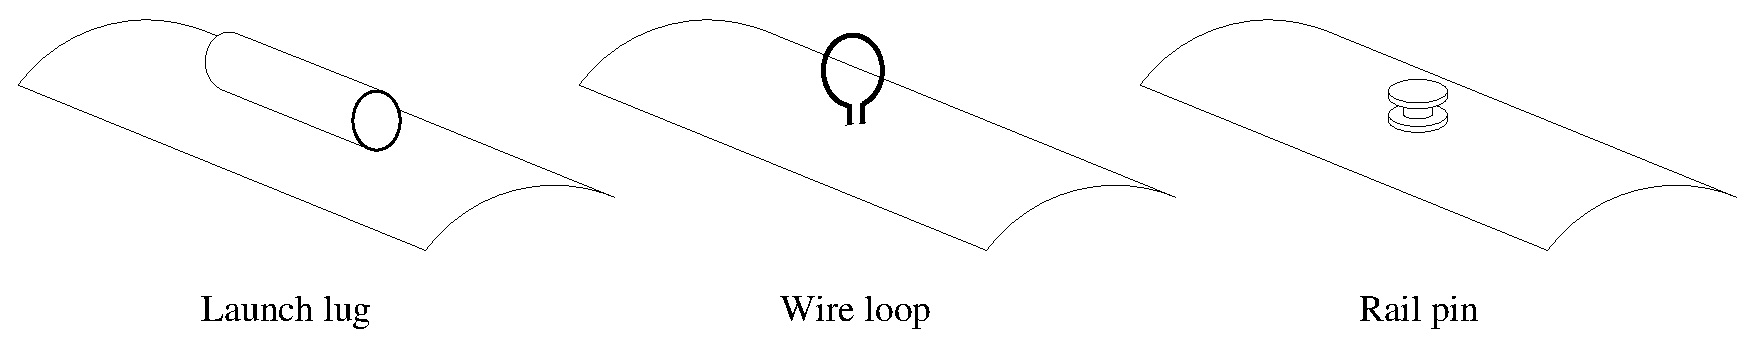
\epsfig{file=figures/components/launch-guides,width=12cm}
\caption{Three types of common launch guides.}
\label{fig-launch-guides}
\end{figure}


A launch lug that is long enough that no appreciable airflow occurs
through the lug may be considered a solid cylinder next to the main
rocket body.  A rectangular protrusion that has a length at least
twice its height has a drag coefficient of 0.74, with reference area
being its frontal area~\cite[p.~5-8]{hoerner}.  The drag coefficient
varies proportional to the stagnation pressure as in the case of a
blunt cylinder in free airflow, presented in
Appendix~\ref{app-blunt-cylinder-drag}.

A wire held perpendicular to airflow has instead a drag coefficient of
1.1, where the reference area is the planform area of the
wire~\cite[p.~3-11]{hoerner}.  A wire loop may be thought of as a
launch lug with length and wall thickness equal to the thickness of
the wire.  However, in this view of a launch lug the reference area
must not include the inside of the tube, since air is free to flow
within the loop.

These two cases may be unified by changing the used reference area as
a function of the length of the tube $l$.  At the limit $l=0$ the
reference area is the simple planform area of the loop, and when the
length is greater than the diameter $l>d$ the reference area includes
the inside of the tube as well.  The slightly larger drag coefficient
of the wire may be taken into account as a multiplier to the blunt
cylinder drag coefficient.

Therefore the drag coefficient of a launch guide can be approximately
calculated by
%
\begin{equation}
(C_{D\bullet})_{\rm parasitic} = 
\max\{1.3-0.3\;l/d, 1\} \cdot (C_{D\bullet})_{\rm stag}
\end{equation}
%
where $(C_{D\bullet})_{\rm stag}$ is the stagnation pressure
coefficient calculated in equation~(\ref{eq-blunt-cylinder-drag}), and
the reference area is
%
\begin{equation}
A_{\rm parasitic} = \pi r_{ext}^2 - \pi r_{int}^2 \cdot
\max\{1-l/d,0\}.
\end{equation}

This approximation may also be used to estimate the drag of rail
pins.  A circular pin protruding from a wall has a drag coefficient of
0.80~\cite[p.~5-8]{hoerner}.  Therefore the drag of the pin is
approximately equal to that of a lug with the same frontal area.  The
rail pins can be approximated in a natural manner as launch lugs with
the same frontal area as the pin and a length equal to their
diameter.




\subsection{Axial drag coefficient}
\label{sec-axial-drag}

The total drag coefficient may be calculated by simply scaling the
coefficients to a common reference area and adding them together:
%
\begin{equation}
C_{D_0} = \sum_T \frac{A_T}{\Aref}(C_{D\bullet})_T
 + (C_D)_{\rm friction}
\end{equation}
%
where the sum includes the pressure, base and parasitic drags.  The
friction drag was scaled to the reference area \Aref\ already in
equation~(\ref{eq-friction-drag-scale}).

This yields the total drag coefficient at zero angle of attack.  At an
angle of attack the several phenomena begin to affect the drag.
More frontal area is visible to the airflow, the pressure gradients
along the body change and fin-tip vortices emerge.  On the other hand,
the drag force is no longer axial, so the axial drag force is less
than the total drag force.

Based on experimental data an empirical formula was produced for
calculating the axial drag coefficient at an angle of attach $\alpha$
from the zero-angle drag coefficient.  The scaling function is a
two-part polynomial function that starts from 1 at $\alpha=0^\circ$,
increases to 1.3 at $\alpha=17^\circ$ and then decreases to zero at
$\alpha=90^\circ$; the derivative is also zero at these points.  Since
the majority of the simulated flight is at very small angles of
attack, this approximation provides a sufficiently accurate estimate
for the purposes of this thesis.


\section{Tumbling bodies}
\label{sec-tumbling-bodies}

% Renaming of test vs. models here:
%
% #1  ->  test 2
% #2  ->  test 3
% #3  ->  test 5
% #4  ->  test 4
% #5  ->  test 6
%
% Test 1 failed to produce a reliable result.  Dimensions:
% n=3, Cr=50, Ct=25, s=50, l0=10, d=18, l=74, m=8.1

In staged rockets the lower stages of the rocket separate from the
main rocket body and descend to the ground on their own.  While large
rockets typically have parachutes also in lower stages, most model
rockets rely on the stages falling to the ground without any recovery
device.  As the lower stages normally are not aerodynamically stable,
they tumble during descent, significantly reducing their speed.

This kind of tumbling is difficult if not impossible to model in
6-DOF, and the orientation is not of interest anyway.
For simulating the descent of aerodynamically unstable stages, it is
therefore sufficient to compute the average aerodynamic drag of
the tumbling lower stage.

While model rockets are built in very peculiar forms, staged rockets
are typically much more conservative in their design.  The lower
stages are most often formed of just a body tube and fins.  Five such
models were constructed for testing their descent aerodynamic drag.

Models \#1 and \#2 are identical except for the number of fins.  \#3
represents a large, high-power booster stage.  \#4 is a body tube
without fins, and \#5 fins without a body tube.

\begin{table}
\caption{Physical properties and drop results of the lower stage models}
\label{tab-lower-stages}
\begin{center}
\parbox{80mm}{
\begin{tabular}{cccccc}
Model       & \#1 & \#2 & \#3 & \#4 & \#5 \\
\hline
No. fins    & 3   & 4   & 3   & 0   & 4    \\
$C_r$ / mm  & 70  & 70  & 200 & -   & 85   \\
$C_t$ / mm  & 40  & 40  & 140 & -   & 85   \\
$s$ / mm    & 60  & 60  & 130 & -   & 50   \\
$l_0$ / mm  & 10  & 10  & 25  & -   & -    \\
$d$ / mm    & 44  & 44  & 103 & 44  & 0    \\
$l$ / mm    & 108 & 108 & 290 & 100 & -    \\
$m$ / g     & 18.0& 22.0& 160 & 6.8 & 11.5 \\
\hline
$v_0$ / m/s & 5.6 & 6.3 & 6.6 & 5.4 & 5.0  \\
\end{tabular}
}
\parbox{50mm}{
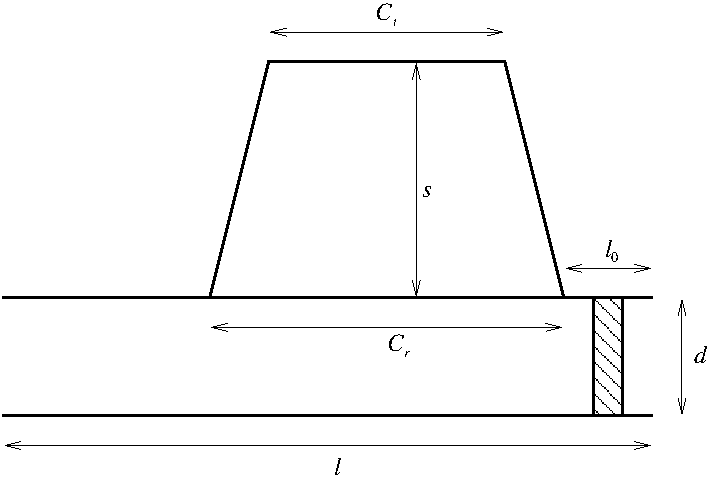
\epsfig{file=figures/lower-stage/lower-stage,width=50mm}
}
\end{center}
\end{table}

The models were dropped from a height of 22 meters and the drop
was recorded on video.  From the video frames the position of
the component was determined and the terminal velocity $v_0$
calculated with an accuracy of approximately $\pm 0.3\;\rm m/s$.
During the drop test the temperature was -5$^\circ$C, relative
humidity was 80\% and the dew point -7$^\circ$C.  Together these yield
an air density of $\rho = 1.31\rm\;kg/m^3$.  The physical properties
of the models and their terminal descent velocities are listed in
Table~\ref{tab-lower-stages}.

For a tumbling rocket, it is reasonable to assume that the drag force
is relative to the profile area of the rocket.  For body tubes the
profile area is straightforward to calculate.  For three and four fin
configurations the minimum profile area is taken instead.

Based on the results of models \#4 and \#5 it is clear that the
aerodynamic drag coefficient (relative to the profile area) is
significantly different for the body tube and fins.  Thus we assume
the drag to consist of two independent components, one for the fins
and one for the body tube.

At terminal velocity the drag force is equal to that of gravity:
%
\begin{equation}
\frac{1}{2}\rho v_0^2\; (C_{D,f}A_f  + C_{D,bt}A_{bt}) = mg
\end{equation}
%
The values for $C_{D,f}$ and $C_{D,bt}$ were varied to optimize the
relative mean square error of the $v_0$ prediction, yielding a result
of $C_{D,f} = 1.42$ and $C_{D,bt} = 0.56$.  Using these values, the
predicted terminal velocities varied between $3\%\ldots14\%$ from the
measured values.

During optimization it was noted that changing the error function
being optimized had a significant effect on the resulting fin drag
coefficient, but very little on the body tube drag coefficient.  It is
assumed that the fin tumbling model has greater inaccuracy in this
aspect.

It is noteworthy that the body tube drag coefficient 0.56 is exactly
half of that of a circular cylinder perpendicular to the
airflow~\cite[p.~3-11]{hoerner}. This is expected of a cylinder that
is falling at a random angle of attack.  The fin drag coefficient 1.42
is also similar to that of a flat plate 1.17 or an open hemispherical
cup 1.42 \cite[p.~3-17]{hoerner}.

The total drag coefficient $C_D$ of a tumbling lower stage is obtained
by combining and scaling the two drag coefficient components:
%
\begin{equation}
C_D = \frac{C_{D,f}A_f  + C_{D,bt}A_{bt}}{\Aref}
\end{equation}
%
Here $A_{bt}$ is the profile area of the body, and $A_f$ the effective
fin profile area, which is the area of a single fin multiplied by the
efficiency factor.  The estimated efficiency factors for various
numbers of fins are listed in Table~\ref{tab-lower-stage-fins}.

\begin{table}
\caption{Estimated fin efficiency factors for tumblig lower stages}
\label{tab-lower-stage-fins}
\begin{center}
\begin{tabular}{cc}
Number  & Efficiency \\
of fins & factor     \\
\hline
1 & 0.50 \\
2 & 1.00 \\
3 & 1.50 \\
4 & 1.41 \\
5 & 1.81 \\
6 & 1.73 \\
7 & 1.90 \\
8 & 1.85 \\
\hline
\end{tabular}
\end{center}
\end{table}




\chapter{Flight simulation}
\label{chap-simulation}

In this chapter the actual flight simulation is analyzed.  First in
Section~\ref{sec-atmospheric-properties} methods for simulating
atmospheric conditions and wind are presented.  Then in
Section~\ref{sec-flight-modeling} the actual simulation procedure is
developed.



\section{Atmospheric properties}
\label{sec-atmospheric-properties}

In order to calculate the aerodynamic forces acting on the rocket it
is necessary to know the prevailing atmospheric conditions.  Since the
atmosphere is not constant with altitude, a model must be developed to
account for the changes.  Wind also plays an important role in the
flight of a rocket, and therefore it is important to have a realistic
wind model in use during the simulation.


\subsection{Atmospheric model}

The atmospheric model is responsible to estimating the atmospheric
conditions at varying altitudes.  The properties that are of most
interest are the density of air $\rho$ (which is a scaling parameter
to the aerodynamic coefficients via the dynamic pressure
$\frac{1}{2}\rho v^2$) and the speed of sound $c$ (which affects the
Mach number of the rocket, which in turn affects its aerodynamic
properties).  These may in turn be calculated from the air pressure
$p$ and temperature $T$.

Several models exist that define standard atmospheric conditions as a
function of altitude, including the Internaltional Standard
Atmosphere (ISA)~\cite{international-standard-atmosphere} and the
U.S. Standard Atmosphere~\cite{US-standard-atmosphere}.  These two
models yield identical temperature and pressure profiles for altitudes
up to 32~km.

The models are based on the assumption that air follows the ideal gas
law
%
\begin{equation}
\rho = \frac{Mp}{RT}
\end{equation}
%
where $M$ is the molecular mass of air and $R$ is the ideal gas
constant.  From the equilibrium of hydrostatic forces the differential
equation for pressure as a function of altitude $z$ can be found as
%
\begin{equation}
\dif p = -g_0 \rho \dif z = -g_0 \frac{Mp}{RT} \dif z
\label{eq-pressure-altitude}
\end{equation}
%
where $g_0$ is the gravitational acceleration.  If the temperature of
air were to be assumed to be constant, this would yield an exponential
diminishing of air pressure.

The ISA and U.S. Standard Atmospheres further specity a standard
temperature and pressure at sea level and a temperature profile for
the atmosphere.  The temperature profile is given as eight
temperatures for different altitudes, which are then linearly
interpolated.  The temperature profile and base pressures for the ISA
model are presented in Table~\ref{table-ISA-model}.  These values
along with equation~(\ref{eq-pressure-altitude}) define the
temperature/pressure profile as a function of altitude.

\begin{table}
\caption{Layers defined in the International Standard
  Atmosphere~\cite{wiki-ISA-layers}}
\label{table-ISA-model}
\begin{center}
\begin{tabular}{ccccl}
\hline
Layer & Altitude$^\dagger$ & Temperature & Lapse rate &
                                                \multicolumn{1}{c}{Pressure} \\
      &  m       &  $^\circ$C  & $^\circ$C/km & \multicolumn{1}{c}{Pa} \\
\hline
0     & 0        & $+15.0$     & $-6.5$       & 101\s325 \\
1     & 11\s000  & $-56.5$     & $+0.0$       & \num22\s632 \\
2     & 20\s000  & $-56.5$     & $+1.0$       & \num\num5\s474.9 \\
3     & 32\s000  & $-44.5$     & $+2.8$       & \num\num\num\s868.02 \\
4     & 47\s000  & \num$-2.5$  & $+0.0$       & \num\num\num\s110.91 \\
5     & 51\s000  & \num$-2.5$  & $-2.8$       & \num\num\num\s\num66.939 \\
6     & 71\s000  & $-58.5$     & $-2.0$       & \num\num\num\s\num\num3.9564 \\
7     & 84\s852  & $-86.2$     &              & \num\num\num\s\num\num0.3734 \\
\hline
\end{tabular}
\end{center}
\vspace{-3mm}
{\footnotesize $^\dagger$ Altitude is the geopotential height which
  does not account for the diminution of gravity at high altitudes.}
\vspace{3mm}
\end{table}

These models are totally static and do not take into account any local
flight conditions.  Many rocketeers may be interested in flight
differences during summer and winter and what kind of effect air pressure
has on the flight.  These are also parameters that can easily be
measured on site when launching rockets.  On the other hand, it is
generally hard to know a specific temperature profile for a specific
day.  Therefore the atmospheric model was extended to allow the user
to specify the base conditions either at mean sea level or at the
altitude of the launch site.  These values are simply assigned to the
first layer of the atmospheric model.  Most model rockets do not
exceed altitudes of a few kilometers, and therefore the flight
conditions at the launch site will dominate the flight.

One parameter that also has an effect on air density and the speed of
sound is humidity.  The standard models do not include any definition
of humidity as a function of altitude.  Furthermore, the effect of
humidity on air density and the speed of sound is marginal.  The
difference in air density and the speed of sound between completely dry
air and saturated air at standard conditions are both less than 1\%.
Therefore the effect of humidity has been ignored.




\subsection{Wind modeling}

Wind plays a critical role in the flight of model rockets.  As has
been seen, large angles of attack may cause rockets to lose a
significant amount of stability and even go unstable.  Over-stable
rockets may weathercock and turn into the wind.  In a perfectly static
atmosphere a rocket would, in principle, fly its entire flight
directly upwards at zero angle of attack.  Therefore, the effect of
wind must be taken into account in a full rocket simulation.

Most model rocketeers, however, do not have access to a full wind
profile of the area they are launching in.  Different layers of air
may have different wind velocities and directions.  Modeling such
complex patterns is beyond the scope of this project. Therefore, the
goal is to produce a realistic wind model that can be specified with
only a few parameters understandable to the user and that covers
altitudes of most rocket flights.  Extensions to allow for multiple
air layers may be added in the future.

In addition to a constant average velocity, wind always has some
degree of turbulence in it.  The effect of turbulence can be modeled
by summing the steady flow of air and a random, zero-mean turbulence
velocity.  Two central aspects of the turbulence velocity are the
amplitude of the variation and the frequencies at which they occur.
Therefore a reasonable turbulence model is achieved by a random
process that produces a sequence with a similar distribution and
frequency spectrum as that of real wind.

Several models of the spectrum of wind turbulence at specific
altitudes exist.  Two commonly used such spectra are the {\it Kaimal}
and {\it von K�rm�n} wind turbulence
spectra~\cite[p.~23]{wind-energy-handbook}:
%
\begin{eqnarray}
\mbox{Kaimal:} & & \frac{S_u(f)}{\sigma_u^2} =
    \frac{4 L_{1u} / U}{(1 + 6fL_{1u}/U)^{5/3}} \label{eq-kaimal-wind} \\
%
\mbox{von K�rm�n:} & & \frac{S_u(f)}{\sigma_u^2} =
    \frac{4 L_{2u} / U}{(1 + 70.8(fL_{2u}/U)^2)^{5/6}} \label{eq-karman-wind}
\end{eqnarray}

Here $S_u(f)$ is the spectral density function of the turbulence
velocity and $f$ the turbulence frequency, $\sigma_u$ the standard
deviation of the turbulence velocity, $L_{1u}$ and $L_{2u}$ length
parameters and $U$ the average wind speed.

Both models approach the asymptotic limit 
$S_u(f)/\sigma_u^2 \sim f^{-5/3}$ quite fast.  Above frequencies of
0.5~Hz the difference between equation~(\ref{eq-kaimal-wind}) and the
same equation without the term 1 in the denominator is less than 4\%.
Since the time scale of a model rocket's flight is quite short, the
effect of extremely low frequencies can be ignored.  Therefore
turbulence may reasonably well be modelled by utilizing 
{\it pink noise} that has a spectrum of $1/f^\alpha$ with $\alpha=5/3$.
True pink noise has the additional useful property of being
scale-invariant.  This means that a stream of pink noise samples may
be generated and assumed to be at any sampling rate while maintaining
their spectral properties.

Discerete samples of pink noise with spectrum $1/f^\alpha$ can be
generated by applying a suitable digital filter to {\it white noise},
which is simply uncorrelated pseudorandom numbers.  One such filter is
the infinite impulse response (IIR) filter presented by
Kasdin~\cite{pink-filter}:
%
\begin{equation}
x_n = w_n - a_1 x_{n-1} - a_2 x_{n-2} - a_3 x_{n-3} - \ldots
\label{eq-pink-generator}
\end{equation}
%
where $x_i$ are the generated samples, $w_n$ is a generated white
random number and the coefficients are computed using
%
\begin{equation}
\begin{array}{rl}
a_0 & = 1 \\
a_k & = \del{k-1-\frac{\alpha}{2}} \frac{a_{k-1}}{k}.
\end{array}
\label{eq-pink-coefficients}
\end{equation}
%
The infinite sum may be truncated with a suitable number of terms.
In the context of IIR filters these terms are calles {\it poles}.
Experimentation showed that already 1--3 poles provides a reasonably
accurate frequency spectrum in the high frequency range.

One problem in using pink noise as a turbulence velocity
model is that the power spectrum of pure pink noise goes to
infinity at very low frequencies.  This means that a long sequence
of random values may deviate significantly from zero.  However, when
using the truncated IIR filter of equation~(\ref{eq-pink-generator}),
the spectrum density becomes constant below a certain limiting
frequency, dependent on the number of poles used.  By adjusting the
number of poles used, the limiting frequency can be adjusted to a value
suitable for model rocket flight.  Specifically, the number of poles
must be selected such that the limiting frequency is suitable at the
chosen sampling rate.  

It is also desirable that the simulation resolution does not affect
the wind conditions.  For example, a simulation with a time step of
10~ms should experience the same wind conditions as a simulation with
a time step of 5~ms.  This is achieved by selecting a constant
turbulence generation frequency and interpolating between the
generated points when necessary.  The fixed frequency was chosen at
20~Hz, which can still simulate fluctuations at a time scale of 0.1
seconds.

\begin{figure}[p]
\centering
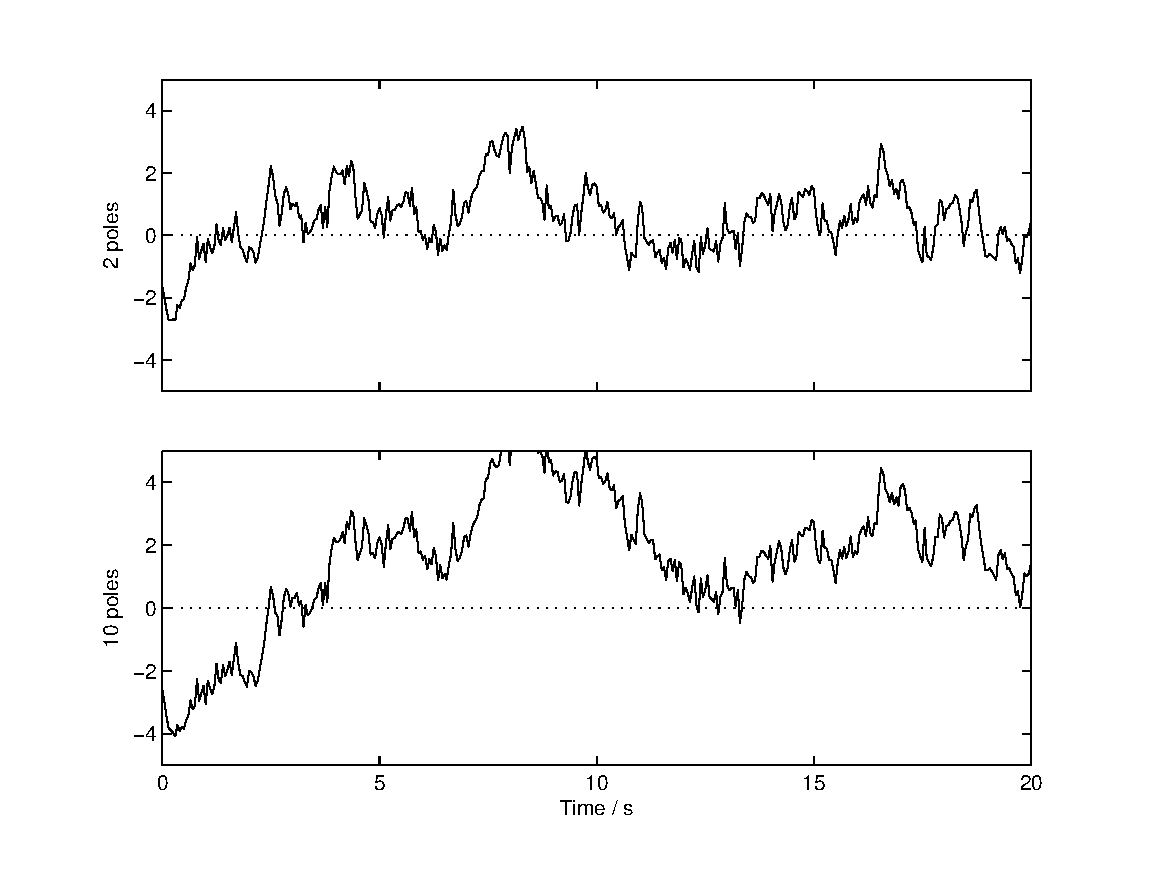
\epsfig{file=figures/wind/pinktime, width=105mm}
\caption{The effect of the number of IIR filter poles on two 20 second
  samples of generated turbulence, normalized so that the two-pole
  sequence has standard deviation one.}
\label{fig-pink-poles}
\end{figure}

\begin{figure}[p]
\centering
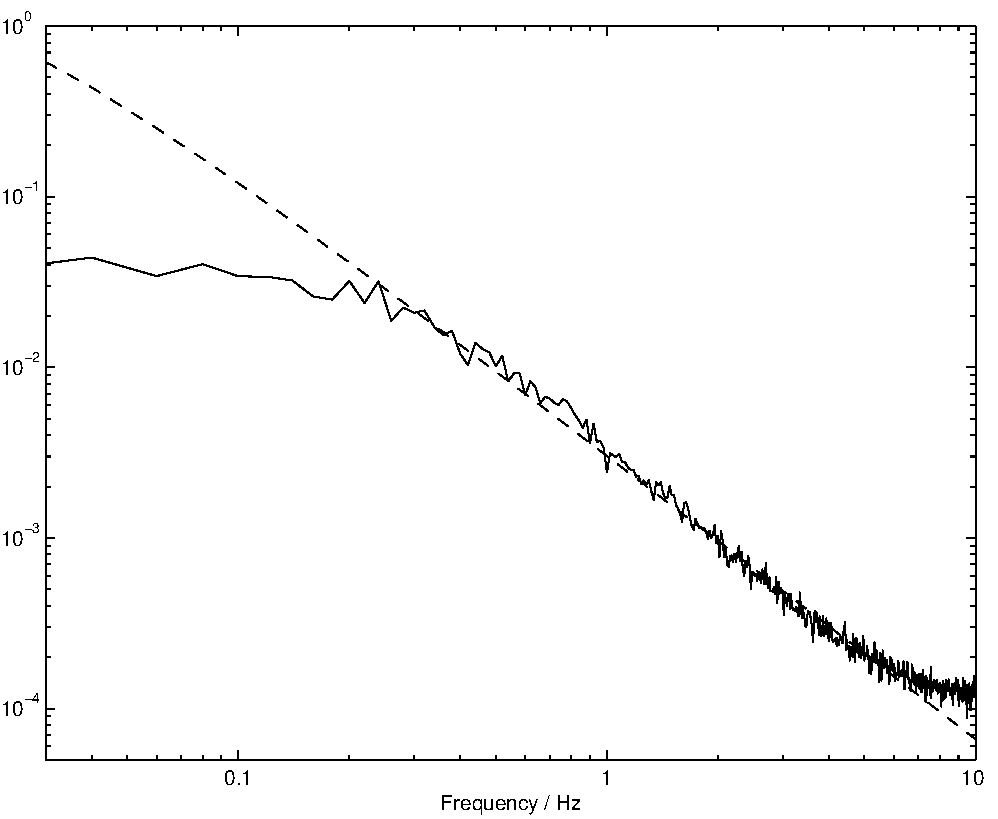
\epsfig{file=figures/wind/pinkfreq, width=95mm}
\caption{The average power spectrum of 100 turbulence
  simulations using a two-pole IIR filter (solid) and the Kaimal
  turbulence spectrum (dashed); vertical axis arbitrary.}
\label{fig-pink-spectrum}
\end{figure}



The effect of the number of poles is depicted in
Figure~\ref{fig-pink-poles}, where two pink noise sequences were
generated from the same random number source with two-pole and
ten-pole IIR filters.  A small number of poles generates values strongly
centered on zero, while a larger number of poles introduces more low
frequency variability.  Since the free-flight time of a typical model
rocket is of the order of 5--30 seconds, it is desireable that the
maximum gust length during the flight is substantially shorter than
this.  Therefore the pink noise generator used by the wind model was
chosen to contain only two poles, which has a limiting frequency of
approximately 0.3~Hz when sampled at 20~Hz.  This means that gusts of
wind longer than 3--5 seconds will be rare in the simulted turbulence,
which is a suitable gust length for modeling typical model rocket
flight. Figure~\ref{fig-pink-spectrum} depicts the resulting pink
noise spectrum of the two-pole IIR filter and the Kaimal spectrum of
equation~(\ref{eq-kaimal-wind}) scaled to match each other.


%, which causes frequency
%components below approximately 0.3~Hz to be subdued.  Therefore, gusts
%of wind longer than 3--5 seconds will be rare in the simulated wind, a
%suitable time scale for the flight of a model rocket.
%Figure~\ref{fig-turbulence}(a) shows a 20 second sample of the
%generated turbulence, normalized to have a standard deviation of one.
%Figure~\ref{fig-turbulence}(b) depicts the actual frequency spectrum
%of the generated turbulence and the Kaimal spectrum of
%equation~(\ref{eq-kaimal-wind}) scaled to match each other.



To simplify the model, the average wind speed is assumed to be
constant with altitude and in a constant direction.  This allows
specifying the model parameters using just the average wind speed and
its standard deviation.  An alternative parameter for specifying the
turbulence amplitude is the {\it turbulence intensity}, which is the
percentage that the standard deviation is of the average wind
velocity,
%
\begin{equation}
I_u = \frac{\sigma_u}{U}.
\end{equation}
%
Wind farm load design standards typically specify turbulence
intensities around 10\ldots20\%~\cite[p.~22]{wind-energy-handbook}.
It is assumed that these intensities are at the top of the range of
conditions in which model rockets are typically flown.

Overall, the process to generate the wind velocity as a function of
time from the average wind velocity $U$ and standard deviation
$\sigma_u$ can be summarized in the following steps:
%
\begin{enumerate}
%\item[Input:]  Average wind velocity $U$ and standard deviation
%  $\sigma_u$.
%
\item Generate a pink noise sample $x_n$ from a Gaussian white noise
  sample $w_n$ using equations~(\ref{eq-pink-generator}) and
  (\ref{eq-pink-coefficients}) with two memory terms included.

\item Scale the sample to a standard deviation one.  This is performed
  by dividing the value by a previously calculated standard deviation
  of a long, unscaled pink noise sequence (2.252 for the two-pole IIR
  filter).

\item The wind velocity at time $n\cdot\Delta t$ ($\Delta t = 0.05\rm~s$)
  is $U_n = U + \sigma_u x_n$.  Velocities in between are interpolated.
\end{enumerate}




\section{Modeling rocket flight}
\label{sec-flight-modeling}


Modeling of rocket flight is based on Newton's laws.  The basic forces
acting upon a rocket are gravity, thrust from the motors and
aerodynamic forces and moments.  These forces and moments are
calculated and integrated numerically to yield a simulation over a
full flight.

Since most model rockets fly at a maximum a few kilometers high, the
curvature of the Earth is not taken into account.  Assuming a flat
Earth allows us to use simple Cartesian coordinates to represent the
position and altitude of the rocket.  As a consequence, the coriolis
effect when flying long distances north or south is not simulated
either.



\subsection{Coordinates and orientation}

During a rocket's flight many quantities, such as the aerodynamical
forces and thrust from the motors, are relative to the rocket itself,
while others, such as the position and gravitational force, are more
naturally described relative to the launch site.  Therefore two sets
of coordinates are defined, the {\it rocket coordinates}, which are
the same as used in Chapter~\ref{chap-aerodynamics}, and 
{\it world coordinates}, which is a fixed coordinate system with the
origin at the position of launch.

The position and velocity of a rocket are most naturally maintained as
Cartesian world coordinates.  Following normal convensions, the
$xy$-plane is selected to be parallel to the ground and the $z$-axis
is chosen to point upwards.  In flight dynamics of aircraft the
$z$-axis often points towards the earth, but in the case of rockets it
is natural to have the rocket's altitude as the $z$-coordinate.

Since the wind is assumed to be unidirectional and the Coriolis effect
is ignored, it may be assumed that the wind is directed along the
$x$-axis.  The angle of the launch rod may then be positioned relative
to the direction of the wind without any loss of generality.

Determining the orientation of a rocket is more complicated.  A
natural choise for defining the orientation would be to use the
spherical coordinate zenith and azimuth angles $(\theta, \phi)$ and an
additional roll angle parameter.  Another choise common in aviation is
to use {\it Euler angles}~\cite{wiki-euler-angles}.  However, both of
these systems have notable shortcomings.  Both systems have
singularity points, in which the value of some parameter is
ambiguous.  With spherical coordinates, this is the direction of the
$z$-axis, in which case the azimuth angle $\phi$ has no effect on the
position.  Rotations that occur near these points must often be
handled as special cases.  Furthermore, rotations in spherical
coordinate systems contain complex trigonometric formulae which are
prone to programming errors.

The solution to the singularity problem is to introduce an extra
parameter and an additional constraint to the system.  For example,
the direction of a rocket could be defined by a three-dimensional unit
vector $(x,y,z)$ instead of just the zenith and azimuth angles.  The
additional constraint is that the vector must be of unit length.  This
kind of representation has no singularity points which would require
special consideration.

Furthermore, Euler's rotation theorem states that a rigid body can be
rotated from any orientation to any other orientation by a single
rotation around a specific axis~\cite{wiki-euler-rotation-theorem}.
Therefore instead of defining quantities that define the orientation
of the rocket we can define a three-dimensional rotation that rotates
the rocket from a known reference orientation to the current
orientation. This has the additional advantage that the same rotation
and its inverse can be used to transform any vector between world
coordinates and rocket coordinates.

A simple and efficient way of descibing the 3D rotation is by using
{\it unit quaternions}.  Each unit quaternion corresponds to a unique
3D rotation, and they are remarkably simple to combine and use.  The
following section will present a brief overview of the properties of
quaternions.

The fixed reference orientation of the rocket defines the rocket
pointing towards the positive $z$-axis in world coordinates and an
arbitrary but fixed roll angle.  The orientation of the rocket is then
stored as a unit quaternion that rotates the rocket from this
reference orientation to its current orientation.  
This rotation can also be used to transform vectors from world
coordinates to rocket coordinates and its inverse from rocket
coordinates to world coordinates.  (Note that the rocket's initial
orientation on the launch pad may already be different than its
reference orientation if the launch rod is not completely vertical.)




\subsection{Quaternions}

{\it Quaternions} are an extension of complex numbers into four
dimensions.  The usefulness of quaternions arises from their use in
spatial rotations.  Similar to the way multiplication with a complex
number of unit length $e^{i\phi}$ corresponds to a rotation of angle
$\phi$ around the origin on the complex plane, multiplication with
unit quaternions correspond to specific 3D rotations around an axis.
A more thorough review of quaternions and their use in spatial
rotations is available in Wikipedia~\cite{wiki-quaternion-rotations}.

The typical notation of quaternions resembles the addition of a scalar
and a vector:
%
\begin{equation}
q = w + x\vi + y\vj + z\vk = w + \vect v
\end{equation}
%
Addition of quaternions and multiplication with a scalar operate as
expected.  However, the multiplication of two quaternions is
non-commutative (in general $ab \neq ba$) and follows the rules
%
\begin{equation}
\vi^2 = \vj^2 = \vk^2 = \vi\vj\vk = -1.
\end{equation}
%
As a corollary, the following equations hold:
%
\begin{equation}
\begin{array}{rl}
\vi\vj = \vk  \hspace{15mm}& \vj\vi = -\vk \\
\vj\vk = \vi  \hspace{15mm}& \vk\vj = -\vi \\
\vk\vi = \vj  \hspace{15mm}& \vi\vk = -\vj 
\end{array}
\end{equation}
%
The general multiplication of two quaternions becomes
%
\begin{equation}
\begin{array}{rl}
(a + b\vi + c\vj + d\vk)(w + x\vi + y\vj + z\vk)\;\; =
 &   (aw-bx-cy-dz) \\
 & + (ax+bw+cz-dy)\;\vi \\
 & + (ay-bz+cw+dx)\;\vj \\
 & + (az+by-cx+dw)\;\vk
\end{array}
\end{equation}
%
while the norm of a quaternion is defined in the normal manner
%
\begin{equation}
|q| = \sqrt{w^2+x^2+y^2+z^2}.
\end{equation}

The usefulness of quaternions becomes evident when we consider a
rotation around a vector $\vect u$, $|\vect u|=1$ by an angle $\phi$.
Let
%
\begin{equation}
q = \cos\frac{\phi}{2} + \vect u \sin\frac{\phi}{2}.
\label{eq-rotation-quaternion}
\end{equation}
%
Now the previously mentioned rotation of a three-dimensional vector
$\vect v$ defined by $\vi$, $\vj$ and $\vk$ is equivalent to the
quaternion product
%
\begin{equation}
\vect v \mapsto q\vect v q^{-1}.
\end{equation}
%
Similarly, the inverse rotation is equivalent to the transformation
%
\begin{equation}
\vect v \mapsto q^{-1} \vect v q.
\end{equation}
%
The problem simplifies even further, since for unit quaternions
%
\begin{equation}
q^{-1} = (w + x\vi + y\vj + z\vk)^{-1} = w - x\vi - y\vj - z\vk.
\end{equation}
%
Vectors can therefore be considered quaternions with no scalar
component and their rotation is equivalent to the left- and right-sided
multiplication with unit quaternions, requiring a total of 24
floating-point multiplications.  Even if this does not make the
rotations more efficient, it simplifies the trigonometry considerably
and therefore helps reduce programming errors.


\subsection{Mass and moment of inertia calculations}
\label{sec-mass-inertia}

Converting the forces and moments into linear and angluar acceleration
requires knowledge of the rocket's mass and moments of inertia.  The
mass of a component can be easily calculated from its volume and
density.  Due to the highly symmetrical nature of rockets, the rocket
centerline is commonly a principal axis for the moments of inertia.
Furthermore, the moments of inertia around the in the $y$- and
$z$-axes are very close to one another.  Therefore as a simplification
only two moments of inertia are calculated, the longitudal and
rotational moment of inertia.  These can be easily calculated for each
component using standard formulae~\cite{wiki-moments-of-inertia} and
combined to yield the moments of the entire rocket.

This is a good way of calculating the mass, CG and inertia of a rocket
during the design phase.  However, actual rocket components often have
a slightly different density or additional sources of mass such as
glue attached to them.  These cannot be effectively modeled by the
simulator, since it would be extremely tedious to define all these
properties.  Instead, some properties of the components can be
overridden to utilize measured values.

Two properties that can very easily be measured are the mass and
CG position of a component.  Measuring the moments of inertia is a
much harder task.  Therefore the moments of inertia are still computed
automatically, but are scaled by the overridden measurement values.

If the mass of a component is overridden by a measured value, the
moments of inertia are scaled linearly according to the mass.  This
assumes that the extra weight is distributed evenly along the
component.  If the CG position is overridden, there is no knowledge
where the extra weight is at.  Therefore as a best guess the moments
of inertia are updated by shifting the moment axis according to the
parallel axis theorem.

As the components are computed individually and then combined, the
overriding can take place either for individual components or larger
combinations.  It is especially useful is to override the mass and/or CG
position of the entire rocket.  This allows constructing a rocket from
components whose masses are not precisely known and afterwards scaling
the moments of inertia to closely match true values.



\subsection{Flight simulation}

The process of simulating rocket flight can be broken down into the
following steps:

\begin{enumerate}
\setcounter{enumi}{-1}
\item Initialize the rocket in a known position and orientation at
  time $t=0$.
\item Compute the local wind velocity and other atmospheric conditions.
\item Compute the current airspeed, angle of attack, lateral wind
  direction and other flight parameters.
\item Compute the aerodynamic forces and moments affecting the rocket.
\item Compute the effect of motor thrust and gravity.
\item Compute the mass and moments of inertia of the rocket and from
  these the linear and rotational acceleration of the rocket.
\item Numerically integrate the acceleration to the rocket's position
  and orientation during a time step $\Delta t$ and update the current
  time $t \mapsto t+\Delta t$.
\end{enumerate}

Steps 1--6 are repeated until an end criteria is met, typically until
the rocket has landed.

The computation of the atmospheric properties and instantaneous wind
velocity were discussed in Section~\ref{sec-atmospheric-properties}.
The local wind velocity is added to the rocket velocity to get the
airspeed velocity of the rocket.  By inverse rotation this quantity is
obtained in rocket coordinates, from which the angle of attack and
other flight parameters can be computed.

After the instantaneous flight parameters are known, the aerodynamic
forces can be computed as discussed in
Chapter~\ref{chap-aerodynamics}.  The computed forces are in the
rocket coordinates, and can be converted to world coordinates by
applying the orientation rotation.  The thrust from the motors is
similarly calculated from the thrust curves and converted to world
coordinates, while the direction of gravity is already in world
coordinates.  When all of the the forces and moments acting upon the
rocket are known, the linear and rotational accelerations can be
calculated using the mass and moments of inertia discussed in
Section~\ref{sec-mass-inertia}.

The numerical integration is performed using the Runge-Kutta~4 (RK4)
integration method.  In order to simulate the differential equations
%
\begin{equation}
\begin{split}
x''(t) &= a(t) \\
\phi''(t) &= \alpha(t)
\end{split}
\end{equation}
%
the equation is first divided into first-order equations using the
substitutions $v(t)=x'(t)$ and $\omega(t)=\phi'(t)$:
%
\begin{equation}
\begin{split}
v'(t) &= a(t) \\
x'(t) &= v(t) \\
\omega'(t) &= \alpha(t) \\
\phi'(t)   &= \omega(t)
\end{split}
\end{equation}
%
For brevity, this is presented in the first order representation
%
\begin{equation}
y' = f(y,\; t)
\end{equation}
%
where $y$ is a vector function containing the position and orientation
of the rocket.

Next the right-hand side is evaluated at four positions, dependent on
the previous evaluations:
%
\begin{equation}
\begin{split}
k_1 &= f(y_0,\; t_0) \\
k_2 &= f(y_0 + k_1\:\mbox{$\frac{\Delta t}{2}$},\; 
       t_0 + \mbox{$\frac{\Delta t}{2}$}) \\
k_3 &= f(y_0 + k_2\:\mbox{$\frac{\Delta t}{2}$},\; 
       t_0 + \mbox{$\frac{\Delta t}{2}$}) \\
k_4 &= f(y_0 + k_3\:\Delta t,\; t_0 + \Delta t)
\end{split}
\end{equation}
%
Finally, the result is a weighted sum of these values:
%
\begin{align}
y_1 &= y_0 + \frac{1}{6}\left(k_1+2k_2+2k_3+k_4\right)\,\Delta t \\
t_1 &= t_0 + \Delta t
\end{align}

Computing the values $k_1\ldots k_4$ involves performing steps~1--5
four times per simulation iteration, but results in significantly
better simulation precision.  The method is a fourth-order integration
method, meaning that the error incurred during one simulation step is
of the order  $O(\Delta t^5)$ and of the total simulation 
$O(\Delta t^4)$.  This is a considerable improvement
over, for example, simple Euler integration, which has a total error
of the order $O(\Delta t)$.  Halving the time step in an Euler
integration only halves the total error, but reduces the error of a
RK4 simulation 16-fold.

The example above used a total rotation vector $\phi$ to contain the
orientation of the rocket.  Instead, this is replaced by the rotation
quaternion, which can be utilized directly as a transformation between
world and rocket coordinates.  Instead of updating the total rotation
vector,
%
\begin{equation}
\phi_1 = \phi_0 + \omega\,\Delta t,
\end{equation}
%
the orientation quaternion $o$ is updated by the same amount by
%
\begin{equation}
o_1 = \del{\cos\del{|\omega|\,\Delta t} +
\hat\omega\sin\del{|\omega|\,\Delta t}} \cdot o_0.
\end{equation}
%
The first term is simply the unit quaternion corresponding to the
3D rotation $\omega\,\Delta t$ as in
equation~(\ref{eq-rotation-quaternion}).  It is applied to the
previous value $o_0$ by multiplying the quaternion from the left.
This update is performed both during the calculation of 
$k_2\ldots k_4$ and when computing the final step result.  Finally, in
order to improve numerical stability, the quaternion is normalized to
unit length.

Since most of a rocket's flight occurs in a straight line, rather
large time steps can be utilized.  However, the rocket may encounter
occasional oscillation, which may affect its flight notably.
Therefore the time step utilized is dynamically reduced in cases where
the angular velocity or angular acceleration exceeds a predefined
limit.  This allows utilizing reasonably large time steps for most of
the flight, while maintaining the accuracy during oscillation.


\subsection{Recovery simulation}

All model rockets must have some recovery system for safe landing.
This is typically done either using a parachute or a streamer.  When a
parachute is deployed the rocket typically splits in half, and it is
no longer practical to compute the orientation of the rocket.
Therefore at this point the simulation changes to a simpler, three
degree of freedom simulation, where only the position of the rocket is
computed.

The entire drag coefficient of the rocket is assumed to come from the
deployed recovery devices.  For parachutes the drag coefficient is
by default 0.8~\cite[p.~13-23]{hoerner} with the reference area being the
area of the parachute.  The user can also define their own drag
coefficient.

The drag coefficient of streamers depend on the material, width and
length of the streamer.  The drag coefficient and optimization of
streamers has been an item of much intrest within the rocketry
community, with competitions being held on streamer descent time
durations~\cite{streamer-optimization}.  In order to estimate the drag
coefficient of streamers, a series of experiments were perfomed using
the $40\times40\times120$~cm wind tunnel of
Pollux~\cite{pollux-wind-tunnel}.  The experiments were performed
using various materials, widths and lengths of streamers and at
different wind speeds.  From these results an empirical formula was
devised that estimates the drag coefficient of streamers.  The
experimental results and the derivation of the empirical formula are
presented in Appendix~\ref{app-streamers}.  Validation performed with
an independent set of measurements indicates that the drag coefficient
is estimated with an accuracy of about 20\%, which translates to a
descent velocity accuracy within 15\% of the true value.




\subsection{Simulation events}

Numerous different events may cause actions to be taken during a
rocket's flight.  For example in high-power rockets the burnout or
ignition charge of the first stage's motor may trigger the ignition of
a second stage motor.  Similarly a flight computer may deploy a small
drogue parachute when apogee is detected and the main parachute is
deployed later at a predefined lower altitude.  To accomodate
different configurations a simulation event system is used, where
events may cause other events to be triggered.

Table~\ref{tab-simulation-events} lists the available simulation
events and which of them can be used to trigger motor ignition or recovery
device deployment.  Each trigger event may additionally include a
delay time.  For example, one motor may be configured to ignite at
launch and a second motor to ignite using a timer at 5 seconds after
launch.  Alternatively, a short delay of 0.5--1 seconds may be used to
simulate the delay of an ejection charge igniting the upper stage
motors.

The flight events are also stored along with the simulated flight data
for later analysis.  They are also available to the simulation
listeners, described in Section~\ref{sec-listeners}, to act upon
specific conditions.

\begin{table}
\caption{Simulation events and the actions they may trigger (motor
  ignition or recovery device deployment).}
\label{tab-simulation-events}
%
\begin{center}
\begin{tabular}{ll}
Event description & Triggers \\
\hline
Rocket launch at $t=0$          & Ignition, recovery \\
Motor ignition                  & None \\
Motor burnout                   & Ignition \\
Motor ejection charge           & Ignition, recovery \\
Launch rod cleared              & None \\
Apogee detected                 & Recovery \\
Change in altitude              & Recovery \\
Touchdown after flight          & None \\
Deployment of a recovery device & None \\
End of simulation               & None \\
\hline
\end{tabular}
\end{center}
\end{table}








\chapter{The OpenRocket simulation software}
\label{chap-software}

The flight simulation described in the previous chapters was
implemented in the {\it OpenRocket} simulation
software~\cite{openrocket}.  The software was written entirely in Java
for maximum portability between different operating systems.  A
significant amount of effort was put into making the graphical user
interface (UI) robust, intuitive and easy to use.  As of the first
public release the source code contained over 300 classes and over
47\s000 lines of code (including comments and blank lines).

The software was released under the copyleft GNU General Public
License (GPL)~\cite{gnu-gpl}, allowing everybody access to the source code
and permitting use and modification for any purposes.  The only major
restriction placed is that if a modified version is distributed, the
source code for the modifications must also be available under the GNU
GPL.  This ensures that the program stays free and Open Source; a
company cannot simply take the code, enhance it and start selling it
as their own without contributing anything back to the community.

In this section the basic architectural designs are discussed and the
main features of the UI are explained.



\section{Architectural design}

The software has been split into various components within their own
Java packages.  This enables use of the components without needing the
other components.  For example, all of the UI code is within the
\code{gui} package, and the simulation system can be used
independently of it.


The rocket structure is composed of components, each with their
own class defined within the package \code{rocketcomponent}.  This
provides the base for defining a rocket.  The components are described
in more detail in Section~\ref{sec-rocket-components}.  The simulation
code is separated from the aerodynamic calculation code in the
\code{simulation} and \code{aerodynamics} packages, respectively;
these are discussed in Section~\ref{sec-simulator-calculator}.

The package naming convention recommended in the Java Language
Specification is followed~\cite{java-packages}.  Therefore all package
names discussed herein are relative to the package
\url{net.sf.openrocket}.  For example, the rocket components are
defined in the package \url{net.sf.openrocket.rocketcomponent}.




\subsection{Rocket components}
\label{sec-rocket-components}

The structure of the rocket is split up into {\it components}, for
example nose cones, body tubes and components within the rocket body.
Each component type is defined as a subclass of the abstract
\code{RocketComponent} class.  Each component can contain zero or more
components attached to it, which creates a tree structure containing
the entire rocket design.  The base component of every design is a
\code{Rocket} object, which holds one or more \code{Stage} objects.
These represent the stages of the rocket and hold all of the physical
components.

Inheritance has been highly used in the class hierarchy of the
components in order to combine common features of various components.
There are also some abstract classes, such as \code{BodyComponent},
whose sole purpose currently is to allow future extensions.  The
complete component class hierarchy is presented as a UML diagram in
Figure~\ref{fig-rocketcomponent-uml}, and a more detailed description
of each class is presented in Table~\ref{table-rocketcomponents}.

\begin{sidewaysfigure}
\centering
\hspace{-1cm}
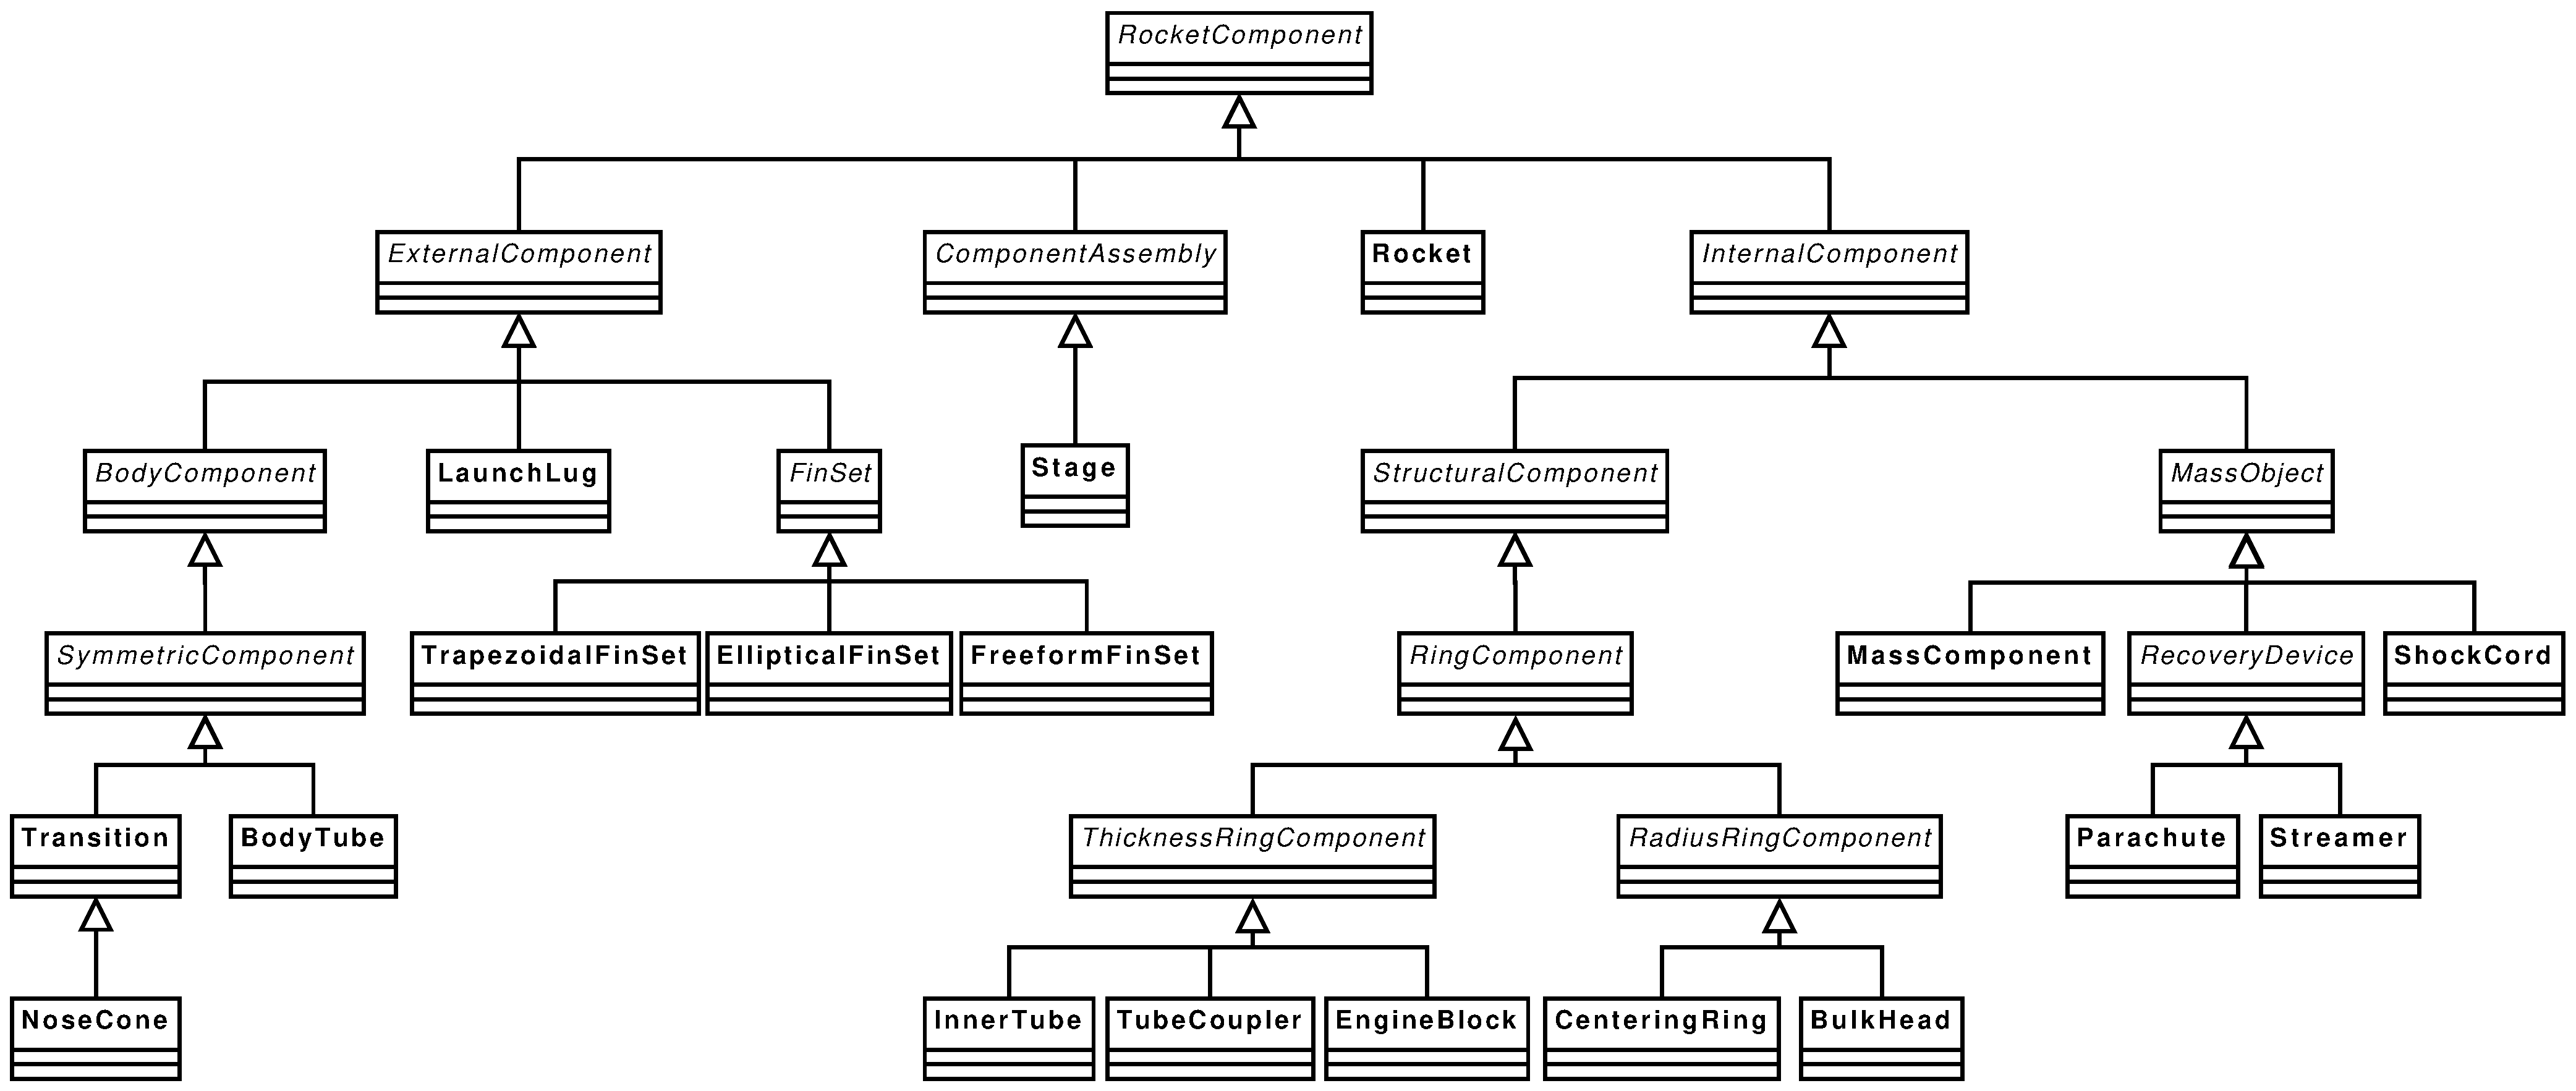
\epsfig{file=figures/software/rocketcomponents,width=20cm}
\caption{A UML diagram of the rocket component classes.  Abstract
  classes are shown in italics.}
\label{fig-rocketcomponent-uml}
\end{sidewaysfigure}


\begin{table}
\caption{Descriptions of the rocket component classes and their
  functionality.  Abstract classes are shown in italics.}
\label{table-rocketcomponents}
\sloppy\footnotesize
\vspace{\baselineskip}
\hspace{-5mm}\begin{tabular}{lp{80mm}}
Component class & Description \\
\hline
\code{\textit{RocketComponent}}: &
  The base class of all components,
  including common features such as child component handling. \\

\hspace{3mm}\code{Rocket}: &
  The base component of a
  rocket design, provides change event notifications. \\

\hspace{3mm}\code{\textit{ComponentAssembly}}: &
  A base component for an assembly of external components.  This could
  in the future be extended to allow multiple rocket bodies next to
  each other. \\

\hspace{6mm}\code{Stage}: &
  A separable stage of the rocket. \\

\hspace{3mm}\code{\textit{ExternalComponent}}: &
  An external component that has an effect on the aerodynamics of the
  rocket. \\

\hspace{6mm}\code{\textit{BodyComponent}}: &
  A portion of the main rocket body, defined in cylindrical coordinates
  by $r = f(x, \theta)$. \\

\hspace{9mm}\code{\textit{SymmetricComponent}}: &
  An axisymmetrical body component. \\

\hspace{12mm}\code{Transition}: &
  A symmetrical transition (shoulder or boattail). \\

\hspace{15mm}\code{NoseCone}: &
  A transition with the initial radius zero. \\

\hspace{12mm}\code{BodyTube}: &
  A cylindrical body tube.  Can be used as a motor mount. \\

\hspace{6mm}\code{\textit{FinSet}}: &
  A set of one or more fins. \\

\hspace{9mm}\code{TrapezoidalFinSet}: &
  A set of trapezoidal fins. \\

\hspace{9mm}\code{EllipticalFinSet}: &
  A set of elliptical fins. \\

\hspace{9mm}\code{FreeformFinSet}: &
  A set of free-form fins. \\

\hspace{6mm}\code{LaunchLug}: &
  A launch lug or rail pin. \\

\hspace{3mm}\code{\textit{InternalComponent}}: &
  An internal component that may affect the mass of the rocket but not
  its aerodynamics. \\

\hspace{6mm}\code{\textit{StructuralComponent}}: &
  A structural internal component, with specific shape and density. \\

\hspace{9mm}\code{\textit{RingComponent}}: &
  A hollow cylindrical component. \\

\hspace{12mm}\code{\textit{ThicknessRingComponent}}: &
  A component defined by an outer radius and shell thickness. \\

\hspace{15mm}\code{InnerTube}: &
  An inner tube.  Can be used as a motor mount and can be clustered. \\

\hspace{15mm}\code{TubeCoupler}: &
  A coupler tube. \\

\hspace{15mm}\code{EngineBlock}: &
  An engine block. \\

\hspace{12mm}\code{\textit{RadiusRingComponent}}: &
  A component defined by an inner and outer radius. \\

\hspace{15mm}\code{CenteringRing}: &
  A ring for centering components. \\

\hspace{15mm}\code{Bulkhead}: &
  A solid bulkhead (inner radius zero). \\

\hspace{6mm}\code{\textit{MassObject}}: &
  An internal component shaped approximately like a solid cylinder and
  with a specific mass. \\

\hspace{9mm}\code{MassComponent}: &
  A generic component with specific mass, for example payload. \\

\hspace{9mm}\code{\textit{RecoveryDevice}}: &
  A recovery device. \\

\hspace{12mm}\code{Parachute}: &
  A parachute. \\

\hspace{12mm}\code{Streamer}: &
  A streamer. \\

\hspace{9mm}\code{ShockCord}: &
  A shock cord with a specified material and length. \\

\hline
\end{tabular}
\end{table}


Additionally four interfaces are defined for the components,
\code{MotorMount}, \code{Clusterable}, \code{Radial\-Parent} and
\code{Coaxial}.  Components implementing the \code{Motor\-Mount}
interface, currently \code{Body\-Tube} and \code{Inner\-Tube}, can
function as motor mounts and have motors loaded in them.  The
\code{Clusterable} interface signifies that the component can be
clustered in various configurations.  Currently only the
\code{Inner\-Tube} component can be clustered.  Components and motors
that are attached to a clustered inner tube are automatically
replicated to all tubes within the cluster.  The \code{Radial\-Parent}
interface allows inner components to automatically identify their
correct inner and outer radii based on their parent and sibling
components.  For example, a coupler tube can automatically detect its
radius based on the inner radius of the parent body tube.
\code{Coaxial} on the other hand provides a generic interface for
accessing and modifying properties of fixed-radius components. 


Since the software functionality is divided into different packages,
all component similarities cannot be directly be exploited through
inheritance.  For example, the method of drawing a nose cone shape
belongs to the \url{gui.rocketfigure} package, however, it can share
the same code that draws a transition.  For these purposes, reflective
programming is used extensively.  The code for drawing both nose cones
and transitions is provided in the class
\code{gui.rocketfigure.SymmetricComponentShapes}, while the simpler
body tube is drawn by the class \code{BodyTubeShapes}.  The correct
class is derived and instantiated dynamically based on the component
class.  This allows easily sharing functionality common to different
components while still having loose coupling between the rocket
structure, presentation, computation and storage methods.




\subsection{Aerodynamic calculators and simulators}
\label{sec-simulator-calculator}

One of the key aspects in the design of the simulation implementation
was extensibility.  Therefore all aerodynamic calculation code is
separated in the package \code{aerodynamics} and all simulation code
is in the package \code{simulator}.  This allows adding new
implementations of the aerodynamic calculators and simulators
independently.  For example, a simulator using Euler integration was
written in the early stages of development, and later replaced by the
Runge-Kutta~4 simulator.  Similarly, a different method of calculating
the aerodynamic forces, such as CFD, could be implemented and used by
the existing simulators.

The basis for all aerodynamic calculations is the interface
\code{Aerodynamic\-Calculator}.  The current implementation, based on
the Barrowman methods, is implemented in the class
\code{Barrowman\-Calculator}.  This implementation caches mid-results
for performance reasons.

Flight simulation is split into the
interfaces \code{Simulation\-Engine}, which is responsible for
maintaining the flow of the simulation and handling events (such as
motor ignition), and \code{Simulation\-Stepper}, which is responsible
for taking individual time steps while simulating (using {\it e.g.}
RK4 iteration).

Similar abstraction has been performed for the atmospheric temperature
and pressure model with the \code{Atmospheric\-Model} interface, the
gravity model with \code{Gravity\-Model}, the wind modelling with
\code{Wind\-Model} and different rocket motor types by the
\code{Motor} class, among others.





\subsection{Simulation listeners}
\label{sec-listeners}

Simulation listeners are pieces of code that can dynamically be
configured to listen to and interact with a simulation while it is
running.  The listeners are called before and after each simulation
step, each simulation event and any calculations performed during
flight simulation.  The listeners may simply gather flight data for
use outside the simulation or modify the rocket or simulation during
the flight.  This allows great potential for extensibility both
internally and externally.

Listeners are used internally for various purposes such as retrieving
flight progress information when the user is running simulations and
cancelling the simulations when necessary.  Implementing such
functionality otherwise would have required a lot of special case
handling directly within the simulation code.

Listeners can also be used to modify the simulation or the rocket
during its flight.  The successor project of Haisun��t� included
an active roll stabilization system, where a flight computer 
measured the roll rate using two magnetometers and used a PID controller
to adjust two auxiliary fins to cancel out any roll produced by
inevitable imperfections in the main fins.  A simulation listener was
written that initially simulated the PID controller purely in Java, which
modified the cant angle of the auxiliary fins during the simulation.
Later a similar listener interfaced the external flight computer
directly using a serial data link.  The listener fed the simulated
flight data to the controller which computed and reported the control
actions back to the simulator.  This system helped identify and fix
numerous bugs in the flight computer software, which would have
otherwise been nearly impossible to fully test.  It is expected that
the simulation listeners will be an invaluable tool for more ambitious
model rocket enthusiasts.

A listener is produced by implementing the \code{Simulation\-Listener}
and optionally \code{Simulation\-Event\-Listener} and
\code{Simulation\-Computation\-Listener} interfaces, or by extending
the \code{Abstract\-Simulation\-Listener} class.  The UI includes the
option of defining custom simulation listeners to be utilized during
flight simulation.


\subsection{Warnings}
\label{sec-warnings}

The aerodynamic calculations and simulations are based on certain
assumptions and simplifications, such as a low angle of attack and a
smooth, continuous rocket body.  The rocket component architecture
makes it possible to create designs that break these assumptions.
Instead of limiting the options of the design, the aerodynamic
calculator and simulator can produce warnings about such issues.
These warnings are presented to the user during the design of the
rocket or after simulations.  It is then left up to the user to judge
whether such violations are significant enough to cast doubt to the
validity of the results.


\subsection{File format}

An XML-based file format was devised for storing the rocket designs
and simulations.  The use of XML allows using many existing tools for
reading and writing the files, allows easy extensibility and makes the
files human-readable.  The user has the option of including all
simulated data in the file, storing the data at specific time
intervals or storing only the simulation launch conditions.  To reduce
the file size, the files can additionally be compressed using the
standard GZIP compression algorithm~\cite{GZIP}.  The files are
compressed and uncompressed automatically by the software.  The file
extension .ORK was chosen for the design files, an abbreviation of the
software name that at the same time had no previous uses as a file
extension.





\section{User interface design}

The user interface was designed with the intent of being robust but
yet easy to use even for inexperienced users.  The main window,
depicted in Figure~\ref{fig-main-window}(a) with the design of the
original Haisun��t� rocket, consists of a schematic drawing of the
rocket, the tree structure of the rocket components and
buttons for adding new components to the structure. Components can
be selected or edited by clicking and double-clicking either the tree
view or the component in the schematic diagram.  The selected
components are drawn in bold to give a visual clue to the position
of the component.

The schematic drawing can be viewed either from the side or from the
rear, can be zoomed in and out and rotated along the centerline.  The
schematic diagram view also presents basic information about the
rocket, such as the design name, length, maximum diameter, mass and
possible warnings about the design. It also calculates the CG and CP
positions continuously during design and shows them both numerically
and on the diagram.  Additionally, a simulation is automatically run
in the background after each modification and the main results are
presented in the lower left corner of the diagram.  Many users are
interested in the maximum altitude or velocity of the rocket, and this
allows an immediate feedback on the effect of the changes they are
making to the design.  The flight information typically takes less
than a second to update.

The upper part of the main window can also be changed to view
simulation results, Figure~\ref{fig-main-window}(b).  Many simulations
can be added with different launch conditions and motor configurations
to investigate their effects.  Each simulation has a row which
presents the basic information about the simulation.  The first column
gives an immediate visual clue to the status of the simulation; a gray
ball indicates that the simulation has not been run yet, green
indicates an up-to-date simulation, red indicates that the design has
been changed after the simulation was run and yellow indicates that
the simulation information was loaded from a file, but that the file
states it to be up-to-date.  The simulations can be run one or several
at a time.  The software automatically utilizes several threads when
running multiple simulations on a multi-CPU computer to utilize the
full processing capacity.

Figure~\ref{fig-various-dialogs} shows two dialogs that are used
to modify and analyze the designs.  The components are edited using a
small dialog window that allows the user to either fill in the exact
numerical values specifying the shape of the component or use sliders
to modify them.  The user can change the units by clicking on them, or
set default values from the preferences.  Different tabs allow control
over the mass and CG override settings, figure color options, motor
mount and cluster options and more.  The Component analysis dialog
shown in the figure can be used to analyze the effect of individual
components on the total stability, drag and roll characteristics of
the rocket.

Similarly, the launch conditions and simulator options can be edited
in the corresponding dialog.  The simulator options also allow the
user to define custom simulation listeners to use during the
simulations.  The simulation edit dialog is also used for later data
analysis.  The simulated data can be plotted in a variety of ways as
shown in Figure~\ref{fig-plotting}.  The user can use predefined plot
settings or define their own.  Up to 15 different variables out of the
47 quantities computed can be plotted at a time.  The variable on the
horizontal axis can be freely selected, and the other variables can be
plotted on one of two vertical axis, on either side of the plot.  The
user can either specify whether a variable should plot on the left or
right axis or let the software decide the most suitable axis.  Typical
plots include the altitude, vertical velocity and acceleration of the
rocket with time or the drag coefficient as a function of the Mach
number.


\begin{figure}
\hspace{-7mm}
\begin{tabular}{m{1mm}m{10cm}}
\hspace{-5mm}(a) &
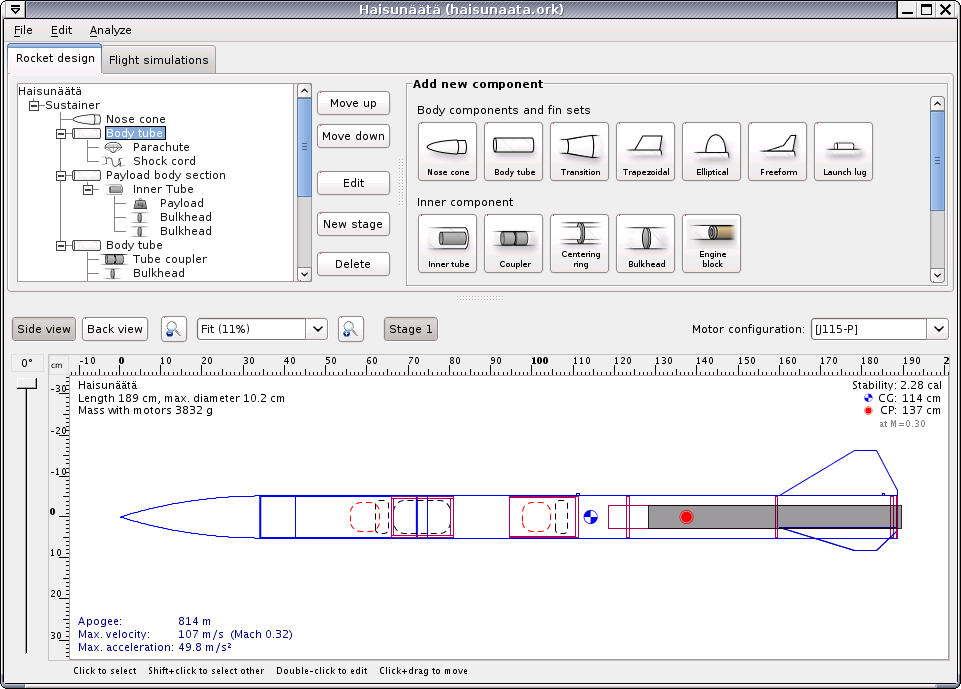
\epsfig{file=figures/pix/openrocket-main-haisunaata,scale=0.5} \\
\hspace{-5mm}(b) &
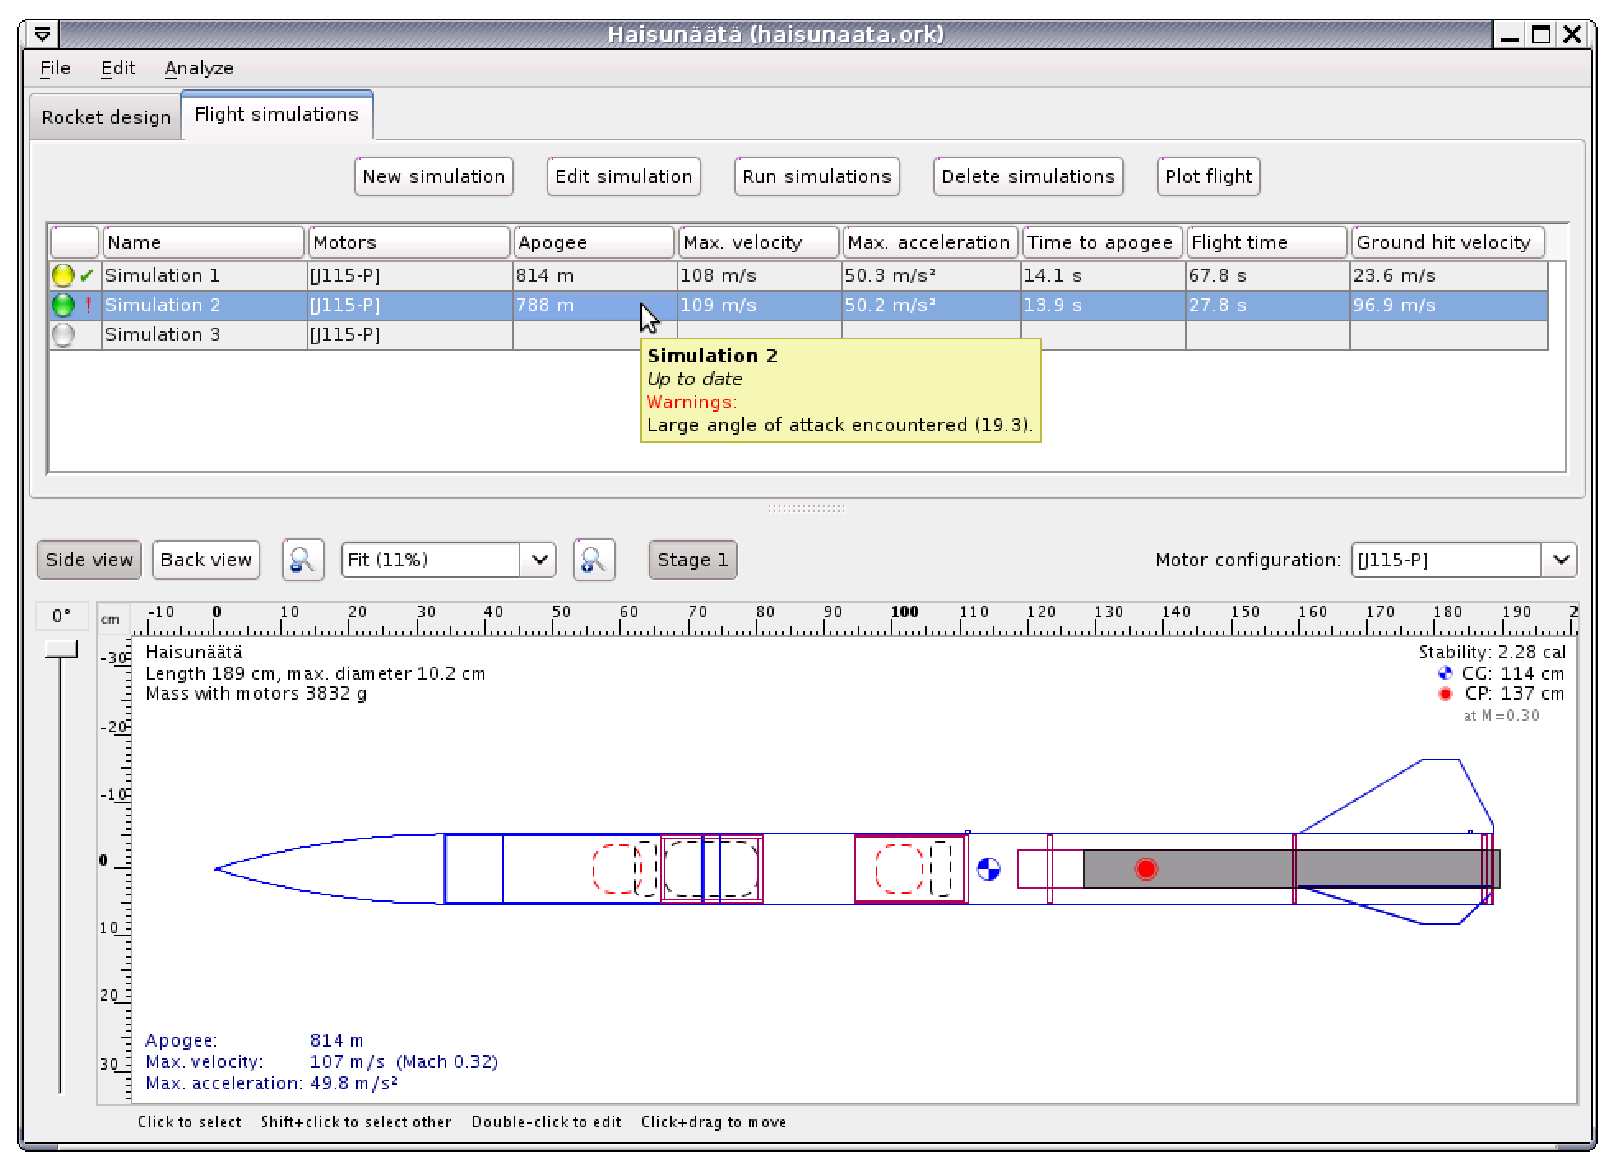
\epsfig{file=figures/pix/openrocket-simulations-haisunaata,scale=0.5}

\end{tabular}
\caption{The main design window of OpenRocket; (a) the design
  view and (b) the simulation view.}
\label{fig-main-window}
\end{figure}

\begin{figure}
\centering
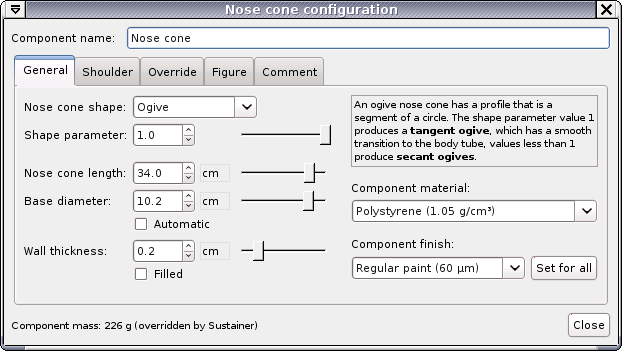
\epsfig{file=figures/pix/openrocket-dialog-edit,scale=0.5}
\vspace{2cm} \\
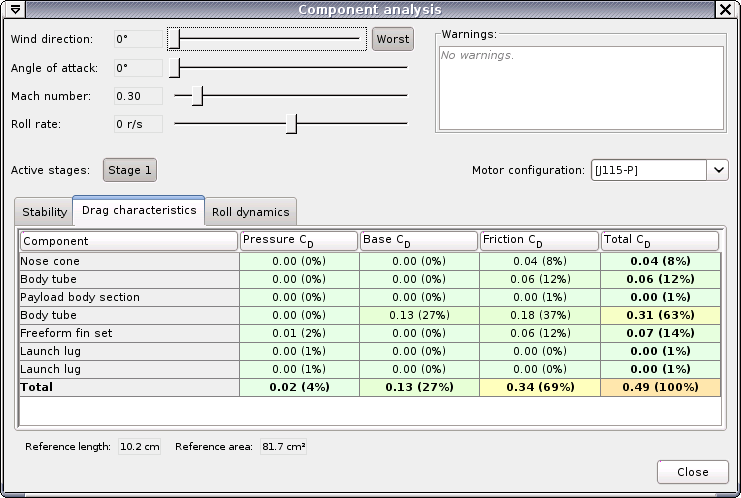
\epsfig{file=figures/pix/openrocket-dialog-analysis,scale=0.5}
\vspace{1cm} \\
\caption{Dialog windows for editing the properties of a nose cone
  and for analyzing the influence of individual components on
  the stability, drag and roll characteristics of the rocket.}
\label{fig-various-dialogs}
\end{figure}

\begin{figure}
\centering
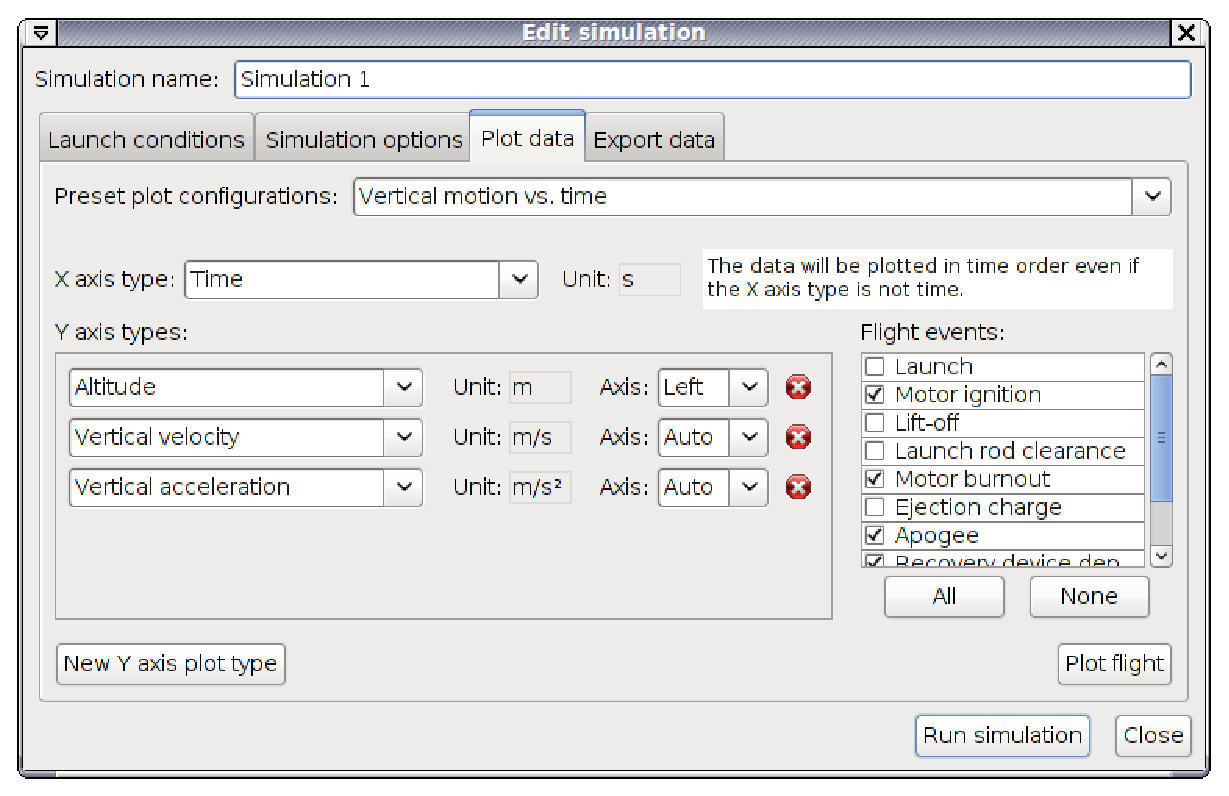
\epsfig{file=figures/pix/openrocket-dialog-plot-options,scale=0.5}
\vspace{2cm} \\
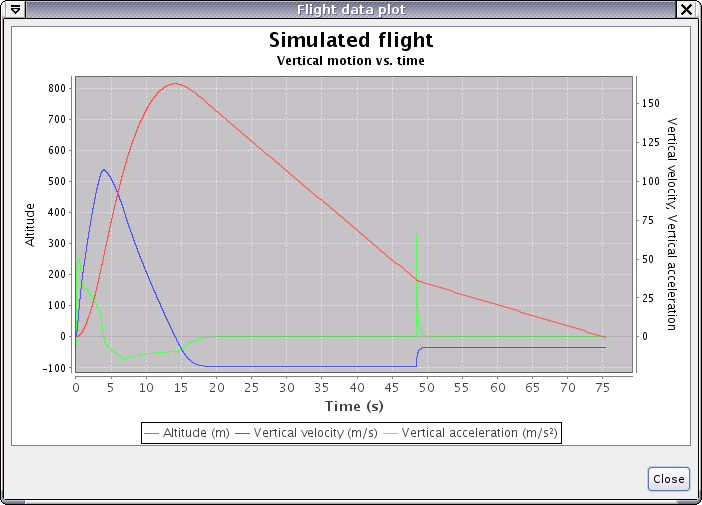
\epsfig{file=figures/pix/openrocket-dialog-plot,scale=0.5}
\vspace{1cm} \\
\caption{Dialog window for changing the simulation plot options and a
  plot of the simulated flight of the Haisun��t� hybrid rocket.}
\label{fig-plotting}
\end{figure}

Advanced users may also export the flight data in CSV format for
further analysis using other tools.

%
%\section{Future enhancements}
%
%Numerous features have been planned and taken into account during the
%design of the software.  Below are listed a few of the planned
%features and how they have been taken into account:
%
%{\it Alternative aerodynamic calculators.}  For example CFD could be
%used to calculate the aerodynamic properties, allowing even better
%simulation accuracy.  The calculators have been abstracted by the
%\code{AerodynamicCalculator} interface so they can easily be
%interchanged.
%
%{\it Alternative simulators.}  These could take into account for
%example the curvature of the Earth and include the Coriolis effect.
%New simulators can be created by implementing the
%\code{Simulation\-Stepper} interface.
%
%{\it Export and import of flight data.}  The simulated data could be
%exported for further analysis as comma separated values (CSV).
%Similarly, experimental data could be imported either from files or
%directly from altimeters.  Support for imported data already exists in
%the core functionalities.
%
%{\it Importing database files.}  The motor database is easily
%extendable to read external thrust curves.  Also data of commercially
%available rocket components could be imported and available in the
%component edit dialog.
%
%{\it Further UI enhancements.}  These could include for example a 3D
%view of the rocket, an animation of the rocket flight, a ``wizard''
%dialog for easily creating new designs, {\it etc.}
%


\chapter{Comparison with experimental data}
\label{chap-experimental}

In order to validate the results produced by the software, several
test flights were made and compared to the results simulated by the
software.  In addition to the software produced, the same simulations
were performed in the current {\it de facto} standard model rocket simulator
RockSim~\cite{rocksim}.  The software used was the free demonstration
version of RockSim version 8.0.1f9.  This is the latest demo version
of the software available at the time of writing.  The RockSim site
states that the demo version is totally equivalent to the normal
version except that it can only be used a limited time and it does not
simulate the rocket's descent after apogee.

Comparisons were performed using both a typical model rocket design,
presented in Section~\ref{sec-comparison-small}, and a large hybrid
rocket, Section~\ref{sec-comparison-large}.  A small model with
canted fins was also constructed and flown to test the roll
simulation, presented in Section~\ref{sec-comparison-roll}.  Finally
in Section~\ref{sec-comparison-windtunnel} some of the the aerodynamic
properties calculated by the software are compared to actual
measurements performed in a wind tunnel.




\section{Comparison with a small model rocket}
\label{sec-comparison-small}

For purposes of gathering experimental flight data, a small model
rocket representing the size and characteristics of a typical model
rocket was constructed and flown in various configurations.  The
rocket model was 56~cm long with a body diameter of 29~mm.  The nose
cone was a 10~cm long tangent ogive, and the fins simple trapezoidal
fins.  The entire rocket was painted using an airbrush but not
finished otherwise and the fin profiles were left rectangular, so as
to represent a typical non-competition model rocket.  The velocity of
the rocket remained below 0.2~Mach during the entire flight.

In the payload section of the rocket was included an Alt15K/WD Rev2
altimeter from PerfectFlite~\cite{perfectflite}.  The altimeter
measures the altitude of the rocket based on atmospheric pressure
changes ten times per second. The manufacturer states the accuracy of
the altimeter to be $\pm (0.25\% + \rm 0.6~m)$.  The altimeter logs
the flight data, which can later be retrieved to a computer for
further analysis. 

Four holes, each 1~mm in diameter were drilled evenly around the
payload body to allow the ambient air pressure to reach the pressure
sensor, as per the manufacturer's instructions.  The rocket was
launched from a 1~m high tower launcher, which removed the need for
any launch lugs.  Figure~\ref{fig-rocket-picture} presents a
picture of the test rocket and the tower launcher.


\begin{figure}
\centering
\parbox{75mm}{\centering  % width 7.4cm
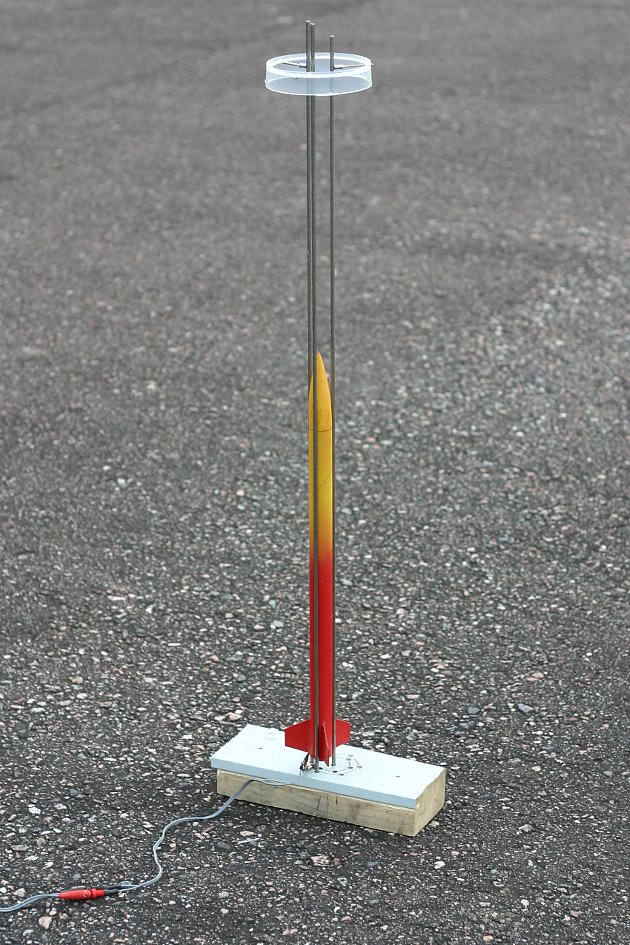
\epsfig{file=figures/pix/rocket-tower,height=11cm} \\ (a)}
\hspace{10mm}
\parbox{35mm}{\centering  % width 3.4cm
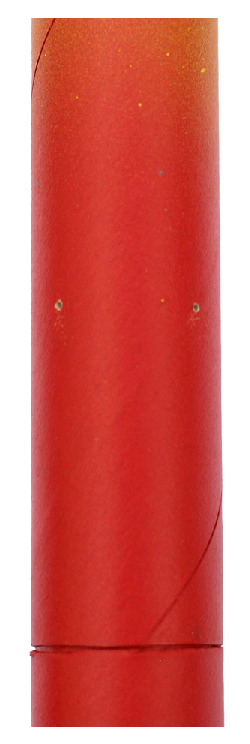
\epsfig{file=figures/pix/rocket-closeup,height=11cm} \\ (b)}
%
\caption{The test rocket awaiting launch on the tower launcher (a) and
  a close-up of its ventilation holes (b).}
\label{fig-rocket-picture}
\end{figure}


A design of the same rocket was created in both OpenRocket and
RockSim.  During construction of the rocket each component was
individually weighed and the weight of the corresponding component
was overridden in the software for maximum accuracy.  Finally, the 
mass and CG position of the entire rocket was overridden with measured
values.

One aspect of the rocket that could not be measured was the average
surface roughness.  In the OpenRocket design the ``regular paint''
finish was selected, which corresponds to an average surface roughness
of 60~\textmu m.  From the available options of ``polished'',
``gloss'', ``matt'' and ``unfinished'' in RockSim, the ``matt'' option
was estimated to best describe the rocket; the corresponding
average surface roughness is unknown.

The rocket was flown using motors manufactured by WECO Feuerwerk
(previously Sachsen Feuerwerk)~\cite{weco-feuerwerk}, which correspond
largely to the motors produced by Estes~\cite{estes}.  The only source
available for the thrust curves of Sachsen Feuerwerk motors was a
German rocketry store~\cite{sf-thrustcurves}, the original source of
the measurements are unknown.  The thrust curve for the C6-3 motor is
quite similar to the corresponding Estes motor, and has a total impulse
of 7.5~Ns.  However, the thrust curve for the B4-4 motor yields a
total impulse of 5.3~Ns, which would make it a C-class motor, while
the corresponding Estes motor has an impulse of only 4.3~Ns.  Both
OpenRocket and RockSim simulated the flight of the rocket using the
SF B4-4 motor over 60\% higher than the apogee of the experimental
results.  It is likely that the thrust curve of the SF B4-4 is wrong,
and therefore the Estes B4-4 motor was used in the simulations in its
stead.


\begin{table}
\caption{Apogee altitude of simulated and experimental flights with
  B4-4 and C6-3 motors.}
\label{tab-flight-results}
\begin{center}
\begin{tabular}{ccccc}
             & \multicolumn{2}{c}{B4-4} & \multicolumn{2}{c}{C6-3} \\
\hline
Experimental~~~~ & 64.0 m &       & 151.5 m &       \\
OpenRocket~~~~   & 74.4 m & +16\% & 161.4 m & +7\%  \\
RockSim~~~~      & 79.1 m & +24\% & 180.1 m & +19\% \\
\hline
\end{tabular}
\end{center}
\end{table}


Figure~\ref{fig-flight-B4} shows the experimental and simulated
results for the flight using a B4-4 motor (simulations using an Estes
motor) and figure~\ref{fig-flight-C6} using a C6-3 motor.  The RockSim
simulations are truncated at apogee due to limitations of the
demonstration version of the software.  A summary of the apogee
altitudes is presented in Table~\ref{tab-flight-results}.  

Both simulations produce a bit too optimistic results. OpenRocket
yielded altitudes 16\% and 7\% too high for the B4-4 and C6-3 motors,
respectively, while RockSim had errors of 24\% and 19\%.  The C6-3
flight is considered to be more accurate due to the ambiguity of the
B4-4 thrust curve.
%
Another feature that can be seen from the graphs is that the estimated
descent speed of the rocket is quite close to the actual descent
speed.  The error in the descent speeds are 7\% and 13\% respectively.


\begin{figure}[p]
\centering
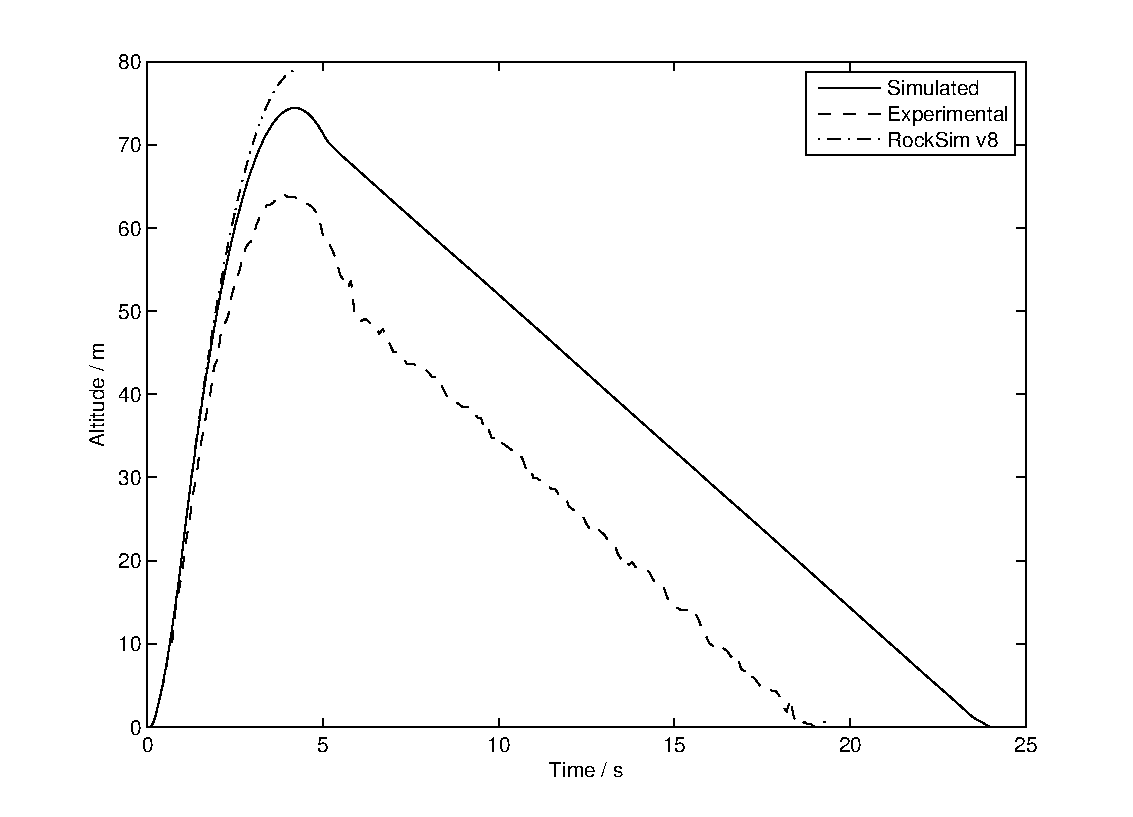
\epsfig{file=figures/experimental/flight-B4-4,width=12cm}
\caption{Experimental and simulated flight using a B4-4 motor.}
\label{fig-flight-B4}
\end{figure}

\begin{figure}[p]
\centering
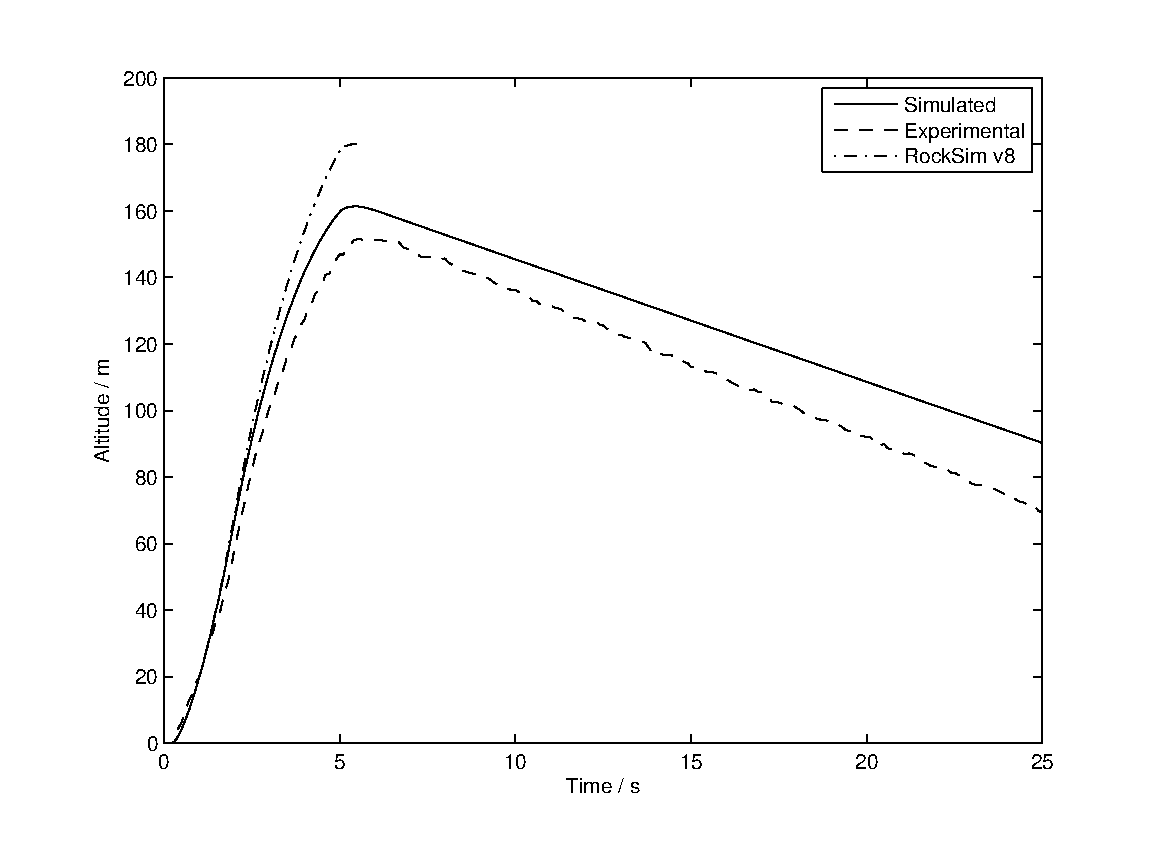
\epsfig{file=figures/experimental/flight-C6-3,width=12cm}
\caption{Experimental and simulated flight using a C6-3 motor.}
\label{fig-flight-C6}
\end{figure}


%       B4-4               C6-3
%Exp    64.0               151.5
%OR     74.4 +10.4 +16%    161.4 +9.9  +7%
%RS     79.1 +15.1 +24%    180.1 +28.6 +19%


The rocket was also launched with a launch lug 24~mm long and 5~mm in
diameter attached first to its mid-body and then next to its fins to
test the effect of a launch lug on the aerodynamic drag.  The apogee
altitudes of the tests were 147.2~m and 149.0~m, which correspond to
an altitude reduction of 2--3\%.  The OpenRocket simulation with such
a launch lug yielded results approximately 1.3\% less than without the
launch lug.




\section{Comparison with a hybrid rocket}
\label{sec-comparison-large}

The second comparison is with the Haisun��t� hybrid
rocket~\cite{haisunaata-launch}, which was launched in September 2008.
The rocket is a HyperLOC 835 model, with a length of 198~cm and a body
diameter of 10.2~cm.  The nose cone is a tangent ogive with a length
of 34~cm, and the kit includes three approximately trapezoidal fins.

The flight computer on board was a miniAlt/WD altimeter by
PerfectFlite~\cite{perfectflite}, with a stated accuracy of 
$\pm0.5\%$.  The flight computer calculates the altitude 20 times per
second based on the atmospheric pressure and stores the data into
memory for later analysis.

The rocket was modeled as accurately as possible with both OpenRocket
and RockSim, but the mass and CG of each component was computed by the
software.  Finally, the mass of the entire rocket excluding the motor
was overridden by the measured mass of the rocket.  The surface
roughness was estimated as the same as for the small rocket,
60~\textmu m in OpenRocket and ``matt'' for RockSim.

Figure~\ref{fig-flight-haisunaata} presents the true flight profile
and that of the simulations.  Both OpenRocket and RockSim estimate a
too low apogee altitude, with an error of 16\% and 12\%,
respectively.  As in the case of the small rocket model, RockSim
produces an estimate 5--10\% higher than OpenRocket.  It remains
unclear which software is more accurate in its estimates.

% Experimental 965m
% OpenRocket 814m
% RockSim  853m


One error factor also affecting this comparison is the use of a hybrid
rocket motor.  As noted in Section~\ref{sec-motors}, the vapor
pressure of the nitrous oxide is highly dependent on temperature,
which affects the thrust of the motor.  This may cause some variation
in the thrust between true flight and motor tests.

\begin{figure}[p]
\centering
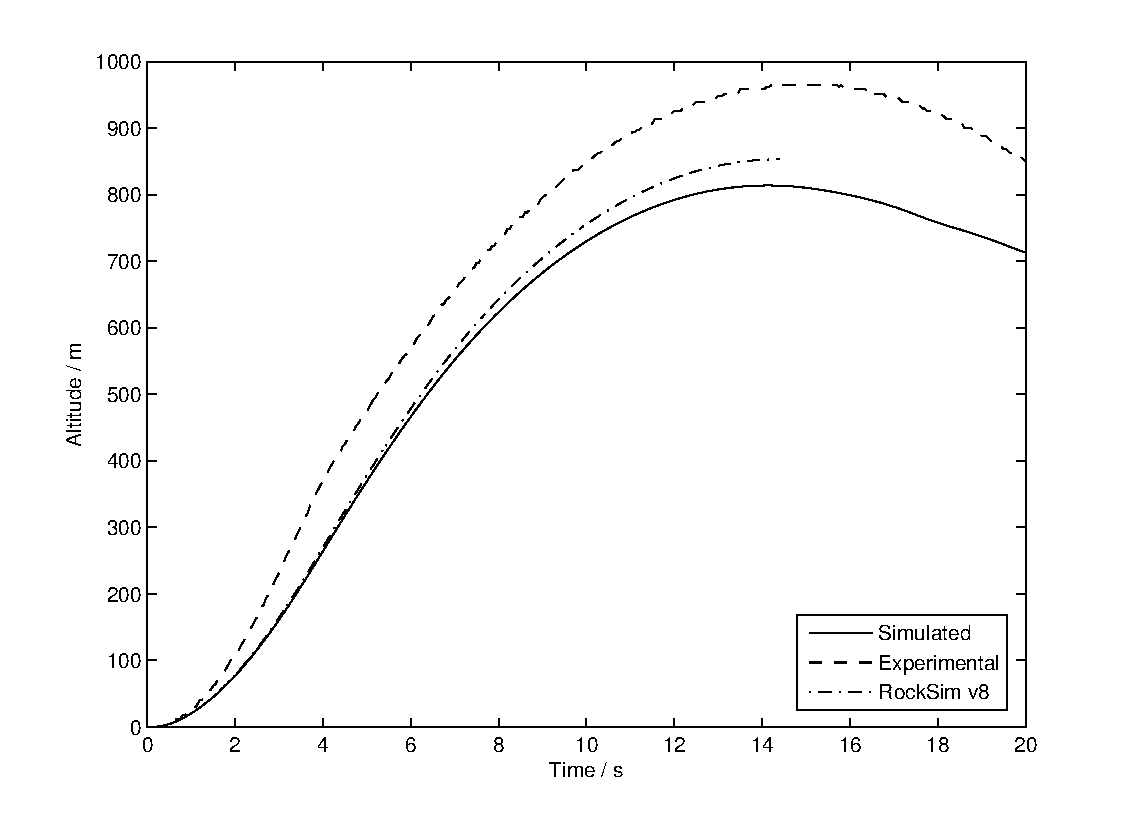
\epsfig{file=figures/experimental/flight-haisunaata,width=12cm}
\caption{Experimental and simulated flight of a hybrid rocket.}
\label{fig-flight-haisunaata}
\end{figure}

\begin{figure}[p]
\centering
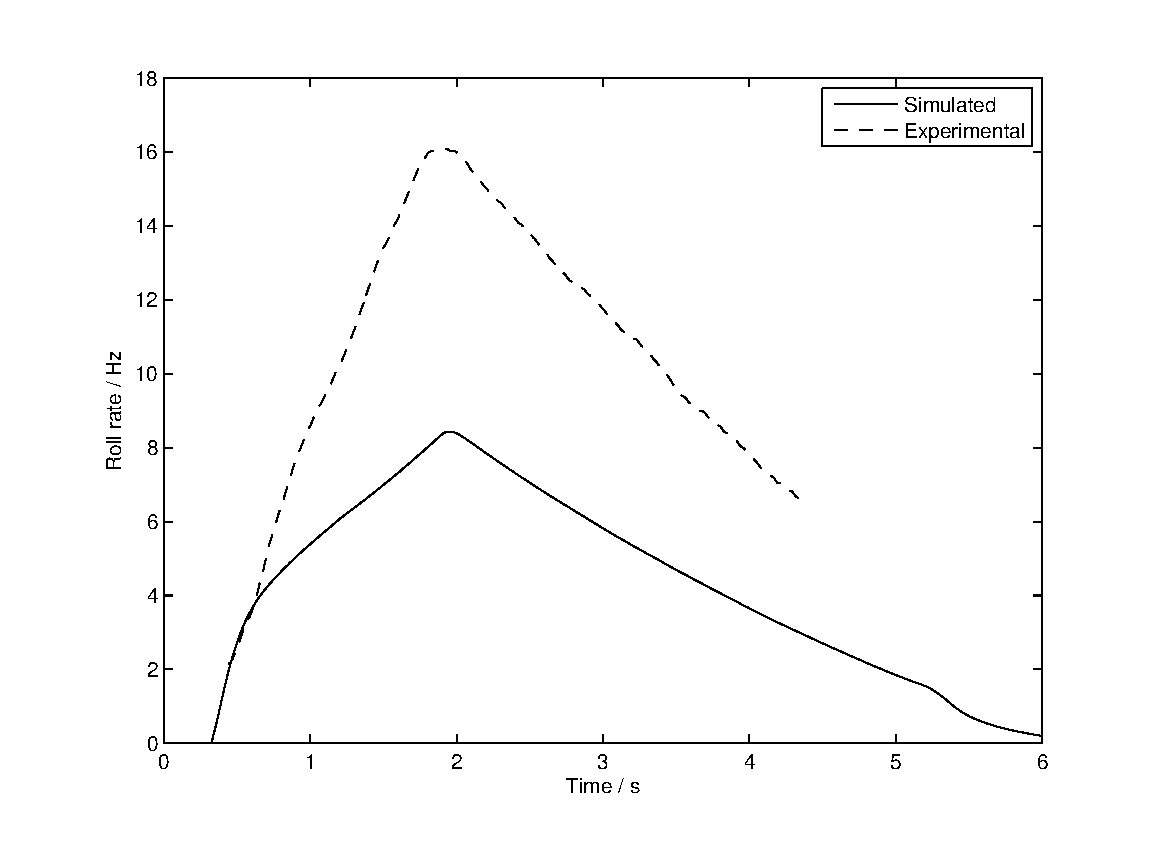
\epsfig{file=figures/experimental/flight-roll-rate,width=12cm}
\caption{Experimental and simulated roll rate results using a C6-3
  motor.}
\label{fig-flight-roll}
\end{figure}



\section{Comparison with a rolling rocket}
\label{sec-comparison-roll}

In order to test the rolling moment computation, a second
configuration of the small model rocket, described in
Section~\ref{sec-comparison-small}, was built with canted fins.  The
design was identical to the previous one, but each fin was canted by
an angle of $5^\circ$.  In addition, the payload section contained a
magnetometer logger, built by Antti~J. Niskanen, that measured the
roll rate of the rocket.  The logger used two Honeywell HMC1051
magnetometer sensors to measure the Earth's magnetic field and store
the values at a rate of 100~Hz for later analysis.  The rocket was
launched from the tower launcher using a Sachsen Feuerwerk C6-3
motor.  Further test flights were not possible since the lower rocket
part was destroyed by a catastrophic motor failure on the second
launch.

After the flight, a spectrogram of the magnetometer data was generated
by dividing the data into largely overlapping segments of 0.4~seconds each,
windowed by a Hamming window, and computing the Fourier transform of
these segments.  For each segment the frequency with the largest power
density was chosen as the roll frequency at the midpoint of the
segment in time.  The resulting roll frequency as a function of time
is plotted in Figure~\ref{fig-flight-roll} with the corresponding
simulated roll frequency.


The simulated roll rate differs significantly from the experimental
roll rate.  During the flight the rocket peaked at a roll rate of 16
revolutions per second, while the simulation has only about half of
this.  The reason for the discrepancy is unknown and would need more
data to analyze.  However, after the test flight it was noticed that
the cardboard fins of the test rocket were slightly curved, which may
have a significant effect on the roll rate.  A more precise test rocket
with more rigid and straight fins would be needed for a more
definitive comparison.  Still, even at a cant angle of $7^\circ$ the
simulation produces a roll rate of only 12~r/s.

Even so, it is believed that including roll in the simulation allows
users to realistically analyze the effect of roll stabilization for
example in windy conditions.


\section{Comparison with wind tunnel data}
\label{sec-comparison-windtunnel}


Finally, the simulated results were compared with experimental wind
tunnel data.  The model that was analyzed by J.~Ferris in the
transonic region~\cite{experimental-transonic} and by C.~Babb and
D.~Fuller in the supersonic region~\cite{experimental-supersonic} is
representative of the Arcas Robin meteorological rocket that has been
used in high-altitude research activities.  The model is 104.1~cm long
with a body diameter of 5.72~cm.  It includes a 27~cm long tangent
ogive nose cone and a 4.6~cm long conical boattail at the rear end,
which reduces the diameter to 3.7~cm.  The rocket includes four
trapezoidal fins, the profiles of which are double-wedges.  For
details of the configuration, refer to~\cite{experimental-transonic}.

The design was replicated in OpenRocket as closely as possible,
given the current limitations of the software.  The most notable
difference is that an airfoil profile was selected for the fins
instead of the double-wedge that is not supported by OpenRocket.  The
aerodynamical properties were computed at the same Mach and Reynolds
numbers as the experimental data.


\begin{figure}[t]
\centering
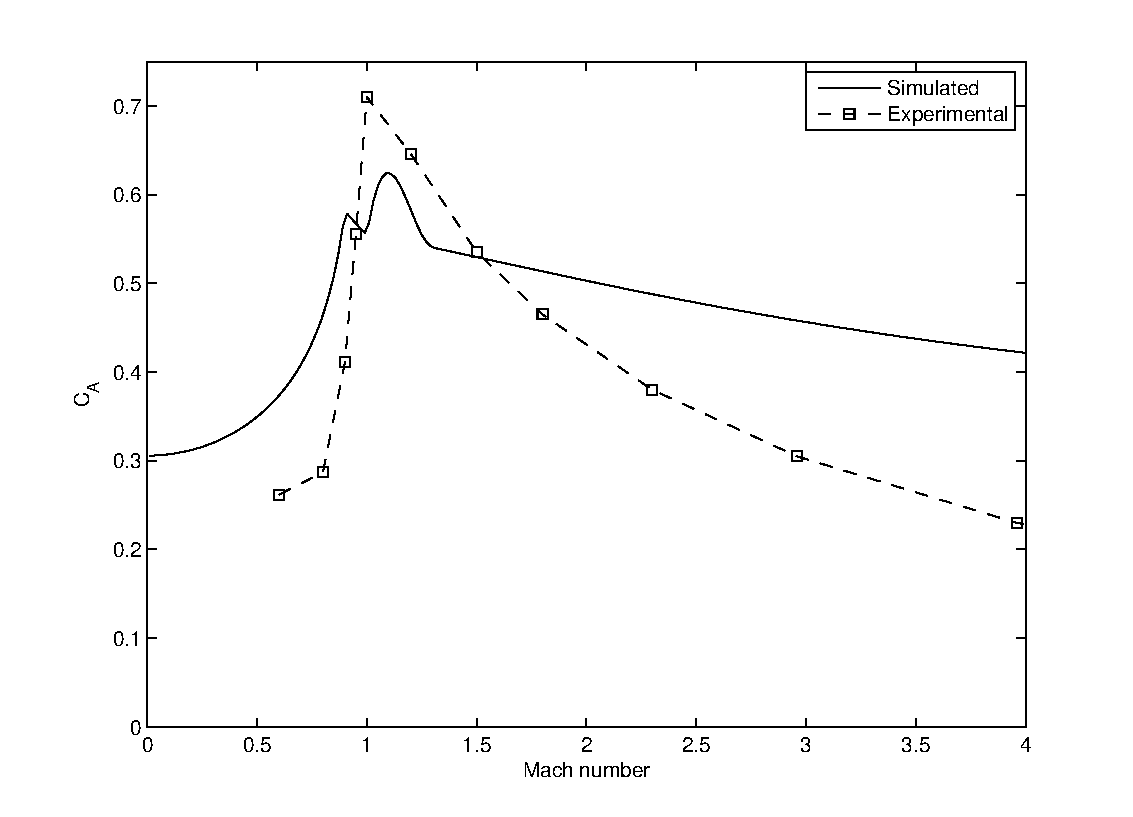
\epsfig{file=figures/experimental/ca-vs-mach,width=11cm}
\caption{Experimental and simulated axial drag coefficient as a
  function of Mach number.}
\label{fig-experimental-CA}
\end{figure}

The most important variables affecting the altitude reached by a
rocket are the drag coefficient and CP location.  The experimental and
simulated axial drag coefficient at zero angle-of-attack is presented
in Figure~\ref{fig-experimental-CA}.  The general shape of the
simulated drag coefficient follows the experimental results.  However,
a few aspects of the rocket break the assumptions made in the
computation methods.  First, the boattail at the end of the rocket
reduces the drag by guiding the air into the void left behind it,
while the simulation software only takes into account the reduction of
base area.  Second, the airfoil shape of the fins affects the drag
characteristic especially in the transonic region, where it produces
the slight reduction peak.  Finally, at higher supersonic speeds the
simulation produces less reliable results as expected, producing a too
high drag coefficient.  Overall, however, the drag coefficient matches
the experimental results with reasonable accuracy, and the results of
actual test flights shown in Sections~\ref{sec-comparison-small} and
\ref{sec-comparison-large} give credence to the drag coefficient
estimation.


\begin{figure}
\centering
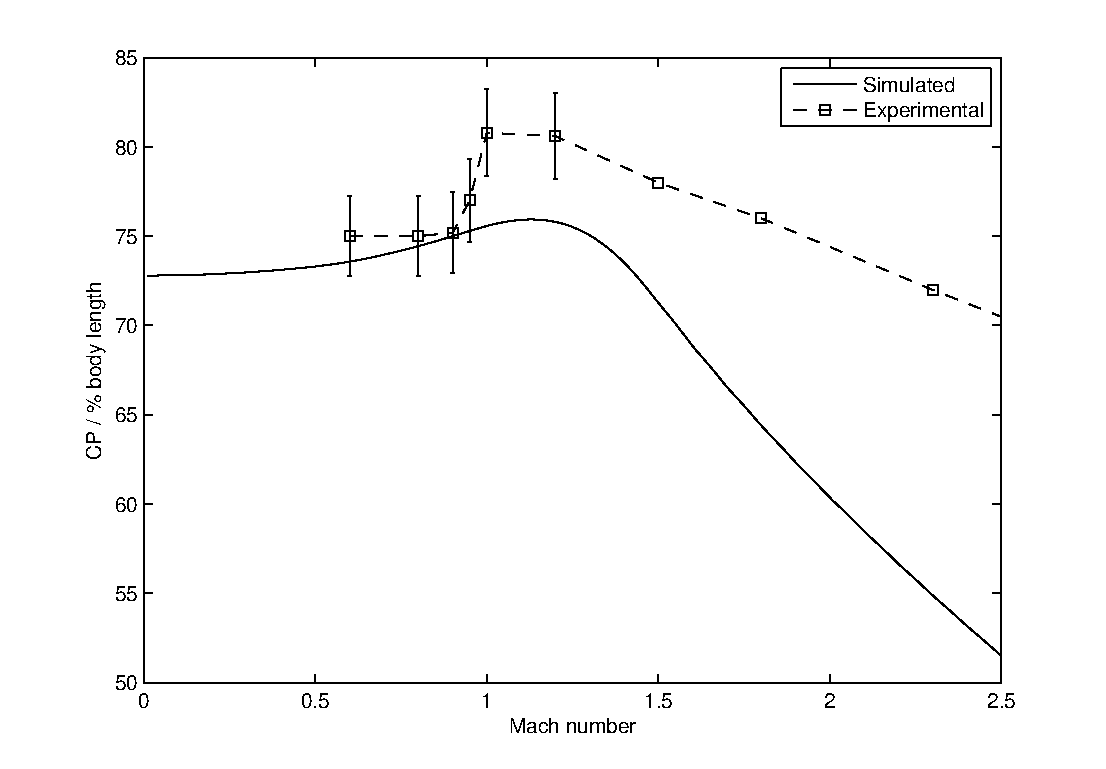
\epsfig{file=figures/experimental/cp-vs-mach,width=12cm} \\
(a) \\
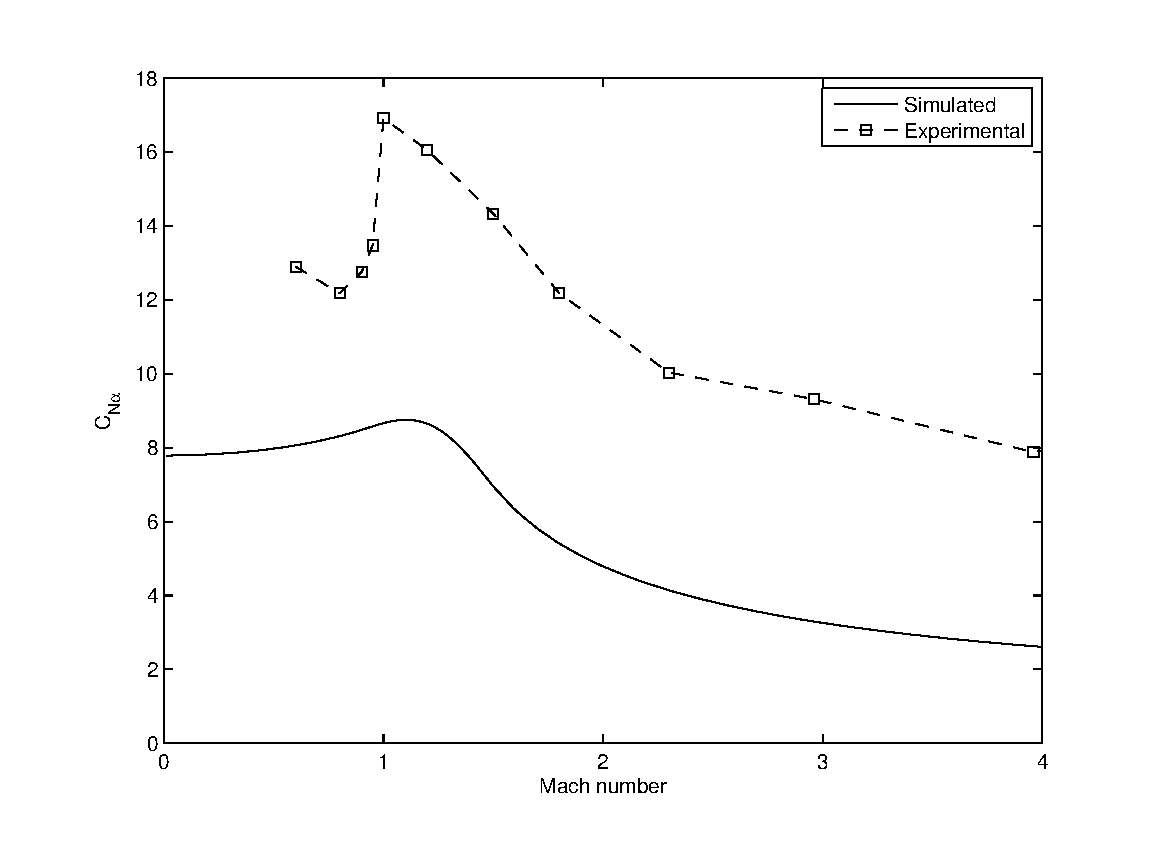
\epsfig{file=figures/experimental/cna-vs-mach,width=12cm} \\
(b)
\caption{Experimental and simulated center of pressure location (a)
  and normal force coefficient derivative (b) as a function of Mach
  number.}
\label{fig-experimental-CP-CNa}
\end{figure}

The CP location as a function of Mach number and the normal force
coefficient derivative \CNa\ are presented in
Figure~\ref{fig-experimental-CP-CNa}.  The 3\% error margins in the
transonic region were added due to difficulty in estimating the normal
force and pitch moment coefficient derivatives from the printed
graphs; in the supersonic region the CP location was provided
directly.  At subsonic speeds the CP location matches the experimental
results to within a few percent.  At higher supersonic speeds the
estimate is too pessimistic, and due to the interpolation this is
visible also in the transonic region.  However, the CP location is
quite reasonable up to about Mach~1.5.

The simulated normal force coefficient derivative is notably lower
than the experimental values.  The reason for this is unknown, since
in his thesis Barrowman obtained results accurate to about 6\%.  The
effect of the lower normal force coefficient on a flight simulation is
that the rocket corrects its orientation slightly slower than in
reality.  The effect on the flight altitude is considered to be small
for typical stable rockets.




\chapter{Conclusion}
\label{chap-conclusion}


Model rocketry is an intriguing sport which combines various fields
ranging from aerodynamic design to model construction to
pyrotechnics.  At its best, it works as an inspiration for youngsters
to study engineering and sciences.

This thesis work provides one of the computer-age tools for everybody
intrested in model rocket design.  Providing everybody free access to
a full-fledged rocket simulator allows many more hobbyists to
experiment with different kinds of rocket designs and become more
involved in the sport.  The most enthusiastic rocketeers may dive
even deeper and get to examine not only the simulation results, but
also how those simulations are actually performed.

The software produced contains an easy-to-use interface, which allows
new users to start experimenting with the minimum effort.  The
back-end is designed to be easily extensible, in anticipation of
future enhancements.  This thesis also includes a step-by-step process
for computing the aerodynamical characteristics of a rocket and for
simulating its flight.  These are the current default implementations
used by the software.

Comparison to experimental data shows that the most important
aerodynamical parameters for flight simulation---the center of
pressure location and drag coefficient---are simulated with an
accuracy of approximately 10\% at subsonic velocities.  In this
velocity regime the accuracy of the simulated altitude is on par with
the commercial simulation software RockSim.  While comparison with
supersonic rockets was not possible, it is expected that the
simulation is reasonably accurate to at least Mach~1.5.

The six degree of freedom simulator also allows simulating rocket roll
in order to study the effect of roll stabilization, a feature
not available in other hobby-level rocket simulators.  While the
comparison with experimental data of a rolling rocket was
inconclusive as to its accuracy, it is still expected to give valuable
insight into the effects of roll during flight.

The external listener classes that can be attached to the simulator
allow huge potential for custom extensions.  For example testing the
active roll reduction controller that will be included in the
successor project of Haisun��t� would have been exceedingly difficult
without such support.  By interfacing the actual controller with a
simulated flight environment it was possible to discover various bugs
in the controller software that would otherwise have gone undetected.

Finally, it must be emphasized that the release of the OpenRocket
software is not the end of this project.  In line with the Open Source
philosophy, it is just the beginning of its development cycle,
where anybody with the know-how can contribute to making OpenRocket an
even better simulation environment.






\clearpage
\vspace*{1cm}
\section*{Acknowledgments}

I would like to express my deepest gratitude to M.Sc.~Timo Sailaranta
for his invaluable advice and consultation on the aerodynamic
simulation of rockets.  Without his input the creation of the
OpenRocket software and Master's thesis would have been exceedingly
laborious.  I would also like to thank Prof.~Rolf Stenberg for
supervising the writing of the Master's thesis.

I am also deeply grateful for my parents Jouni and Riitta, my entire
family, friends and teachers, who have always encouraged me onwards in
my life and studies.  Above all I would like to thank my brother,
Antti~J. Niskanen, for being an inspiration throughout my life and
also for building the magnetometer logger used in the experimental
flights; and my wife Merli Lahtinen, for her patience and loving
understanding for my passion towards rocketry.




\begin{thebibliography}{99}

\bibitem{thesis} Niskanen, S., {\it Development of an Open Source
  model rocket simulation software}, M.Sc. thesis, Helsinki University
  of Technology, 2009.  Available at
  \url{http://openrocket.sourceforge.net/documentation.html}.

\bibitem{stine} Stine, H., Stine, B., {\it Handbook of Model
  Rocketry}, 7th edition, Wiley, 2004.

\bibitem{barrowman-rd} Barrowman, J., Barrowman, J., The
  theoretical prediction of the center of pressure, {\it National
  Association of Rocketry Annual Meet 8}, 1966.  Available at
\url{http://www.apogeerockets.com/Education/downloads/barrowman_report.pdf},
  retrieved 14.5.2009.

\bibitem{barrowman-thesis} Barrowman, J., {\it The practical
  calculation of the aerodynamic characteristics of slender finned
  vehicles}, M.Sc. thesis, The Catholic University of America, 1967.

\bibitem{rocksim} van Milligan, T., RockSim Model Rocket Design and
  Simulation Software, \url{http://www.apogeerockets.com/RockSim.asp},
  retrieved 14.5.2009.

\bibitem{oss-principles} Coar, K., The Open Source Definition
  (Annotated), \url{http://www.opensource.org/docs/definition.php},
  retrieved 14.5.2009.

\bibitem{openrocket} Niskanen, S., The OpenRocket web-site,
  \url{http://openrocket.sourceforge.net/}, retrieved 25.5.2009.

\bibitem{nar-safety-code} Anon., Model Rocket Safety Code,
  \url{http://www.nar.org/NARmrsc.html}, retrieved 14.5.2009.

\bibitem{all-certified-motors} Anon., Combined CAR/NAR/TRA Certified
  Rocket Motors List,
  \url{http://www.nar.org/SandT/pdf/CombinedList.pdf}, retrieved 14.5.2009.

\bibitem{thrust-curve-database} Coker, J., ThrustCurve Hobby Rocket
  Motor Data, \url{http://www.thrustcurve.org/}, retrieved 14.5.2009.

\bibitem{D12-curve} Kane, J., Estes D12,
  \url{http://www.nar.org/SandT/pdf/Estes/D12.pdf}, retrieved 14.5.2009.

\bibitem{haisunaata-launch} Puhakka, A., Haisun��t�---suomalainen
  hybridirakettiprojekti (in Finnish),
  \url{http://haisunaata.avaruuteen.fi/}, retrieved 14.5.2009.

\bibitem{galejs} Galejs, R., Wind instability---What Barrowman left
  out,
  \url{http://projetosulfos.if.sc.usp.br/artigos/sentinel39-galejs.pdf},
  retrieved 14.5.2009.

\bibitem{advanced-model-rocketry} Mandell, G., Caporaso, G., Bengen,
  W., {\it Topics in Advanced Model Rocketry}, MIT Press, 1973.

\bibitem{hoerner} Hoerner, S., {\it Fluid-dynamic drag}, published by
  the author, 1965.
% FLUID-DYNAMIC DRAG
% Practical Information on AERODYNAMICDRAG and HYDRODYNAMIC RESISTANCE
% Sighard F. Hoerner (Dr.-Ing.)
% Published by the Author 1958
%
% Chap II - Skin-friction drag
%   laminaarinen, turbulentti, ym.
% Chap III - Pressure drag
%   forebudy pressure drag for different shapes
%   Base drag C_DB = 0.029/sqrt(C_fB)  forebody-drag coefficient C_fB
% Chap V - Drag of surface imperfections
%   Drag due to surface roughtness
%   Critical roughness
%   Page 5-8, Drag of Individual Protuberances
%     neliskanttinen pala, pituus < korkeus -> CD=1.20
%                          pituus > 2*kork  -> CD=0.74
%                     suhteutettu etupinta-alaan
%     From ref. Tillmann, Rpt KW Inst. G�ttingen, Dec 1944
% Chap VII - Drag due to lift
% Chap VIII - Interference drag
%   Pairs of bodies
% Chap X - Hydrodynamic drag
%   sivu 10-3, siivekkeiden profiilimuotoja!!!
% Chap XIII - Drag of airplane components and accessories
%   Drag of external loads
%   Parachutes
% Chap XV-XVII - subsonic, transsonic, supersonic

\bibitem{barrowman-elliptical-fins} Barrowman, J., Elliptical Fin
  C.P. Equations, {\it Model Rocketry} (Nov 1970).  Available at
  \url{http://www.argoshpr.ch/articles/pdf/EllipticalCP.jpg},
  retrieved 14.5.2009.

\bibitem{appl-comp-aero-fins} Mason, W., Applied Computational
  Aerodynamics,
  \url{http://www.aoe.vt.edu/~mason/Mason_f/CAtxtTop.html}, 
  {\bf pp. A-27--A-28}, retrieved 14.5.2009.

\bibitem{fleeman} Fleeman, E., {\it Tactical missile design}, 2nd
  edition, p.~33, AIAA, 2006.

\bibitem{diederich} Diederich, F., {\it A plan-form parameter for
 correlating certain aerodynamic characteristics of swept ings},
 NACA-TN-2335, 1951.

\bibitem{barrowman-fin} Barrowman, J., {\it FIN A computer program for
  calculating the aerodynamic characteristics of fins at supersonic
  speeds}, {\it NASA-TM X-55523}, 1966.

\bibitem{pettis} Pettis, W., {\it Aerodynamic Characteristics of
  Multiple Fins of Rectangular Planform on a Body of Revolution at
  Mach Numbers of 1.48 to 2.22}, RD-TM-67-5, US Army Missile
  Command, 1967.

\bibitem{experimental-transonic} Ferris, J., {\it Static stability
  investigation of a single- stage sounding rocket at Mach numbers
  from 0.60 to 1.20}, NASA-TN-D-4013, 1967.

\bibitem{triform-fin-data} Monta, W., {\it Aerodynamic
  characteristics at mach numbers from 1.60 to 2.16 of a blunt-nose
  missile model having a triangular cross section and fixed triform
  fins}, NASA-TM-X-2340, 1971.

\bibitem{MIL-HDBK} Anon., {\it Design of aerodynamically stabilized
  free rockets}, MIL-HDBK-762, US Army Missile Command, 1990.

\bibitem{handbook-supersonic-aerodynamics} Anon., {\it Handbook of
  supersonic aerodynamics, Section 8, Bodies of revolution}, 
  NAVWEPS REPORT 1488, 1961.

\bibitem{second-order-shock-expansion-method} Syverston, C., Dennis,
  D., {\it A second-order shock-expansion method applicable to bodies
  of revolution near zero lift}, NACA-TR-1328, 1957.

\bibitem{international-standard-atmosphere} Anon., {\it Standard
  Atmosphere}, ISO~2533:1975, International Organization for
  Standardization, 1975.

\bibitem{US-standard-atmosphere} Anon., {\it U.S. Standard Atmosphere
  1976}, NASA-TM-X-74335; NOAA-S/T-76-1562, 1976.

\bibitem{wiki-ISA-layers}  Anon., International Standard Atmosphere,
  \url{http://en.wikipedia.org/wiki/International_Standard_Atmosphere},
  retrieved 14.5.2009.

\bibitem{wind-energy-handbook} Burton, T., Sharpe, D., Jenkins, N.,
  Bossanyi, E., {\it Wind Energy Handbook}, Wiley, 2001.

\bibitem{pink-filter}  Kasdin, J., Discrete Simulation of Colored
  Noise and Stochastic Processes and $1/f^\alpha$ Power Law Noise
  Generation, {\it Proceedings of the IEEE}, {\bf 83}, No.~5 (1995),
  p. 822.

\bibitem{wiki-euler-angles} Anon., Euler angles,
  \url{http://en.wikipedia.org/wiki/Euler_angles}, retrieved 14.5.2009.

\bibitem{wiki-euler-rotation-theorem} Anon., Euler's rotation theorem,
  \url{http://en.wikipedia.org/wiki/Euler's_rotation_theorem},
  retrieved 14.5.2009.

\bibitem{wiki-quaternion-rotations} Anon., Quaternions and spatial
  rotation,
  \url{http://en.wikipedia.org/wiki/Quaternions_and_spatial_rotation},
  retrieved 14.5.2009.

\bibitem{wiki-moments-of-inertia} Anon., List of moments of inertia,
  \url{http://en.wikipedia.org/wiki/List_of_moments_of_inertia},
  retrieved 14.5.2009.

\bibitem{pollux-wind-tunnel} Niskanen, S., Polluxin tuulitunneli (in
  Finnish), \url{http://pollux.tky.fi/tuulitunneli.html}, retrieved 14.5.2009.

\bibitem{gnu-gpl} Anon., GNU General Public License, Version 3,
  \url{http://www.gnu.org/copyleft/gpl.html}, retrieved 14.5.2009.

\bibitem{java-packages} Anon., Java Language Specification, Chaper 7,
  Packages,
 \url{http://java.sun.com/docs/books/jls/third_edition/html/packages.html#7.7},
  retrieved 14.5.2009.

\bibitem{GZIP} Deutsch, P., {\it GZIP file format specification
  version 4.3}, RFC~1952, \url{http://www.ietf.org/rfc/rfc1952.txt},
  1996.  Retrieved on 14.5.2009.

\bibitem{perfectflite} Anon., Affordable instrumentation for (sm)all
  rockets, \url{http://www.perfectflite.com/}, retrieved 14.5.2009.

\bibitem{weco-feuerwerk} Anon., WECO Feuerwerk,
  \url{http://www.weco-feuerwerk.de/}, retrieved 14.5.2009.

\bibitem{estes} Anon., Estesrockets.com,
  \url{http://www.estesrockets.com/}, retrieved 14.5.2009.

\bibitem{sf-thrustcurves} Anon., Schubdiagramme SF,
  \url{http://www.raketenmodellbautechnik.de/produkte/Motoren/SF-Motoren.pdf},
  14.5.2009.

\bibitem{experimental-supersonic} Babb, C., Fuller, D., {\it Static
  stability investigation of a sounding-rocket vehicle at Mach numbers
  from 1.50 to 4.63}, NASA-TN-D-4014, 1967.

\bibitem{nosecone-cd-data} Stoney, W., {\it Collection of Zero-Lift
  Drag Data on Bodies of Revolution from Free-Flight Investigations}, 
  NASA-TR-R-100, 1961.

\bibitem{streamer-optimization} Kidwell, C., Streamer Duration
  Optimization: Material and Length-to-Width Ratio, {\it National
  Association of Rocketry Annual Meet 43}, 2001.  Available at
  \url{http://www.narhams.org/library/rnd/StreamerDuration.pdf},
  retrieved 14.5.2009.

\end{thebibliography}




\appendix



\chapter{Nose cone and transition geometries}
\label{app-nosecone-geometry}

Model rocket nose cones are available in a wide variety of shapes and
sizes.  In this appendix the most common shapes and their defining
parameters are presented.


\section{Conical}

The most simple nose cone shape is a right circular cone.  They are
easy to make from a round piece of cardboard.  A conical nose cone is
defined simply by its length and base diameter. An additional
parameter is the opening angle $\phi$, shown in
Figure~\ref{fig-nosecone-shapes}(a).  The defining equation of a
conical nose cone is
%
\begin{equation}
r(x) = \frac{x}{L}\cdot R.
\end{equation}


\section{Ogival}

Ogive nose cones have a profile which is an arc of a circle, as shown
in Figure~\ref{fig-nosecone-shapes}(b).  The most common ogive shape
is the {\it tangent ogive} nose cone, which is formed when radius of
curvature of the circle $\rho_t$ is selected such that the joint
between the nose cone and body tube is smooth,
%
\begin{equation}
\rho_t = \frac{R^2+L^2}{2R}.
\end{equation}
%
If the radius of curvature $\rho$ is greater than this, then the
resulting nose cone has an angle at the joint between the nose cone
and body tube, and is called a {\it secant ogive}.  The secant ogives
can also be viewed as a larger tangent ogive with its base cropped.
At the limit $\rho\rightarrow\infty$ the secant ogive becomes a
conical nose cone.

The parameter value $\kappa$ used for ogive nose cones is the ratio of
the radius of curvature of a corresponding tangent ogive $\rho_t$ to
the radius of curvature of the nose cone $\rho$:
%
\begin{equation}
\kappa = \frac{\rho_t}{\rho}
\end{equation}
%
$\kappa$ takes values from zero to one, where $\kappa=1$ produces a
tangent ogive and $\kappa=0$ produces a conical nose cone (infinite
radius of curvature).

With a given length $L$, radius $R$ and parameter $\kappa$ the radius
of curvature is computed by
%
\begin{equation}
\rho^2 = \frac{ \del{L^2+R^2}\cdot
  \del{ \del{\del{2-\kappa}L}^2 + \del{\kappa R}^2 }
}{ 4\del{\kappa R}^2 }.
\end{equation}
%
Using this the radius at position $x$ can be computed as
%
\begin{equation}
r(x) = \sqrt{\rho^2 - \del{L/\kappa - x}^2} - \sqrt{\rho^2-\del{L/\kappa}^2}
\end{equation}



\section{Elliptical}

Elliptical nose cones have the shape of an ellipsoid with one major
radius is $L$ and the other two $R$.  The profile has a shape of a
half-ellipse with major axis $L$ and $R$,
Figure~\ref{fig-nosecone-shapes}(c).  It is a simple geometric shape
common in model rocketry.  The special case $R=L$ corresponds to a
half-sphere.

The equation for an elliptical nose cone is obtained by stretching the
equation of a unit circle:
\begin{equation}
r(x) = R \cdot \sqrt{1-\del{1-\frac{x}{L}}^2}
\end{equation}


\section{Parabolic series}

A parabolic nose cone is the shape generated by rotating a section of
a parabola around a line perpendicular to its symmetry axis,
Figure~\ref{fig-nosecone-shapes}(d).  This is
distinct from a paraboloid, which is rotated around this symmetry
axis (see Appendix~\ref{app-power-series}).  

Similar to secant ogives, the base of a ``full'' parabolic nose cone
can be cropped to produce nose cones which are not tangent with the
body tube.  The parameter $\kappa$ describes the portion of the larger
nose cone to include, with values ranging from zero to one.  The most
common values are $\kappa=0$ for a conical nose cone, $\kappa=0.5$ for
a 1/2~parabola, $\kappa=0.75$ for a 3/4~parabola and $\kappa=1$ for a
full parabola.  The equation of the shape is
%
\begin{equation}
r(x) = R\cdot\frac{x}{L} \del{ \frac{2 - \kappa\frac{x}{L}}
   {2-\kappa}}.
\end{equation}



\section{Power series}
\label{app-power-series}

The power series nose cones are generated by rotating the segment
%
\begin{equation}
r(x) = R\del{\frac{x}{L}}^\kappa
\end{equation}
%
around the x-axis, Figure~\ref{fig-nosecone-shapes}(e).  The parameter
value $\kappa$ can range from zero to one.  Special cases are
$\kappa=1$ for a conical nose cone, $\kappa=0.75$ for a 3/4~power nose
cone and $\kappa=0.5$ for a 1/2~power nose cone or an ellipsoid.
The limit $\kappa\rightarrow0$ forms a blunt cylinder.


\section{Haack series}

In contrast to the other shapes which are formed from rotating
geometric shapes or simple formulae around an axis, the Haack series
nose cones are mathematically derived to minimize the theoretical
pressure drag.  Even though they are defined as a series, two specific
shapes are primarily used, the {\it LV-Haack}\ shape and the 
{\it LD-Haack}\ or {\it Von K�rman}\ shape.  The letters LV and LD
refer to length-volume and length-diameter, and they minimize the
theoretical pressure drag of the nose cone for a specific length and
volume or length and diameter, respectively.  Since the parameters
defining the dimensions of the nose cone are its length and radius,
the Von K�rman nose cone (Figure~\ref{fig-nosecone-shapes}(f)) should,
in principle, be the optimal nose cone shape.

The equation for the series is
%
\begin{equation}
r(x) = \frac{R}{\sqrt{\pi}} \;
  \sqrt{\theta - \frac{1}{2}\sin(2\theta) + \kappa \sin^3\theta}
\end{equation}
%
where
%
\begin{equation}
\theta = \cos^{-1} \del{1-\frac{2x}{L}}.
\end{equation}
%
The parameter value $\kappa=0$ produces the Von K�rman of LD-Haack
shape and $\kappa=1/3$ produces the LV-Haack shape.  In principle,
values of $\kappa$ up to $2/3$ produce monotonic nose cone shapes.
However, since there is no experimental data available for the
estimation of nose cone pressure drag for $\kappa > 1/3$ (see
Appendix~\ref{app-haack-series-pressure-drag}), the selection of the
parameter value is limited in the software to the range 
$0 \ldots 1/3$.


\section{Transitions}

The vast majority of all model rocket transitions are conical.
However, all of the nose cone shapes may be adapted as transition
shapes as well.  The transitions are parametrized with the fore and
aft radii $R_1$ and $R_2$, length $L$ and the optional shape parameter
$\kappa$.

Two choices exist when adapting the nose cones as transition shapes.
One is to take a nose cone with base radius $R_2$ and crop the tip of
the nose at the radius position $R_1$.  The length of the nose cone
must be selected suitably that the length of the transition is $L$.
Another choice is to have the profile of the transition resemble two
nose cones with base radius $R_2-R_1$ and length $L$.  These two
adaptations are called {\it clipped} and {\it non-clipped} transitions,
respectively.  A clipped and non-clipped elliptical transition is
depicted in Figure~\ref{fig-transition-clip}.

For some transition shapes the clipped and non-clipped adaptations are
the same.  For example, the two possible ogive transitions have equal
radii of curvature and are therefore the same.  Specifically, the
conical and ogival transitions are equal whether clipped or not, and
the parabolic series are extremely close to each other.




\begin{figure}[p]
\centering
\begin{tabular}{ccc}

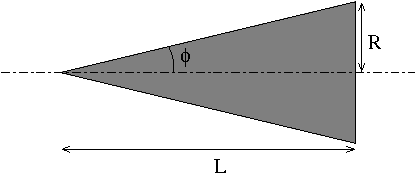
\epsfig{file=figures/nose-geometry/geometry-conical,scale=0.7} &&
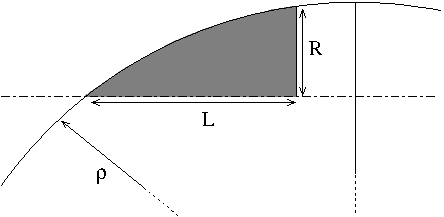
\epsfig{file=figures/nose-geometry/geometry-ogive,scale=0.7} \\
(a) & \hspace{1cm} & (b) \\
&& \\
&& \\
&& \\
%&& \\

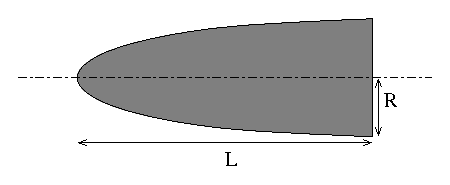
\epsfig{file=figures/nose-geometry/geometry-elliptical,scale=0.7} &&
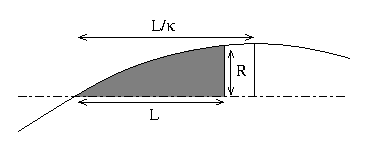
\epsfig{file=figures/nose-geometry/geometry-parabolic,scale=1.0} \\
(c) && (d) \\
&& \\
&& \\
&& \\
%&& \\

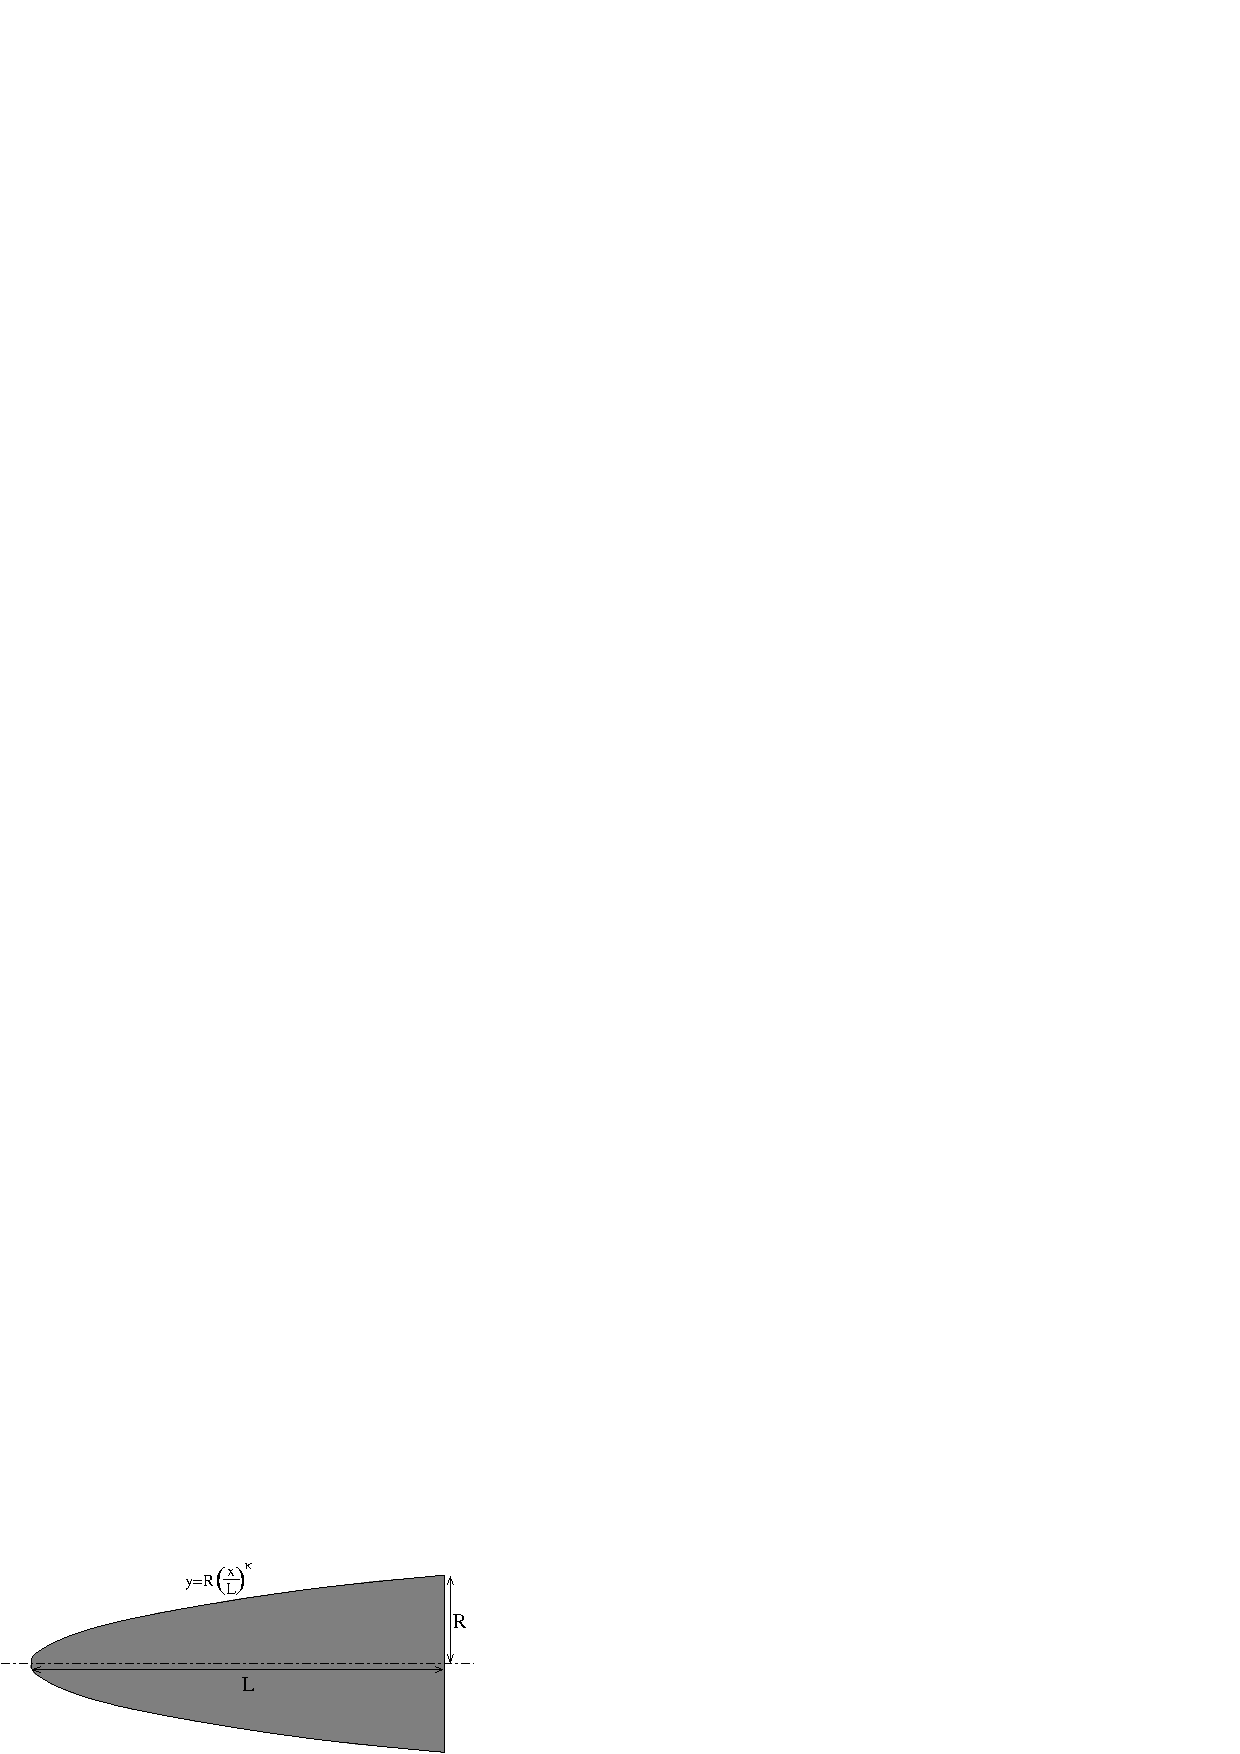
\epsfig{file=figures/nose-geometry/geometry-power,scale=0.6} &&
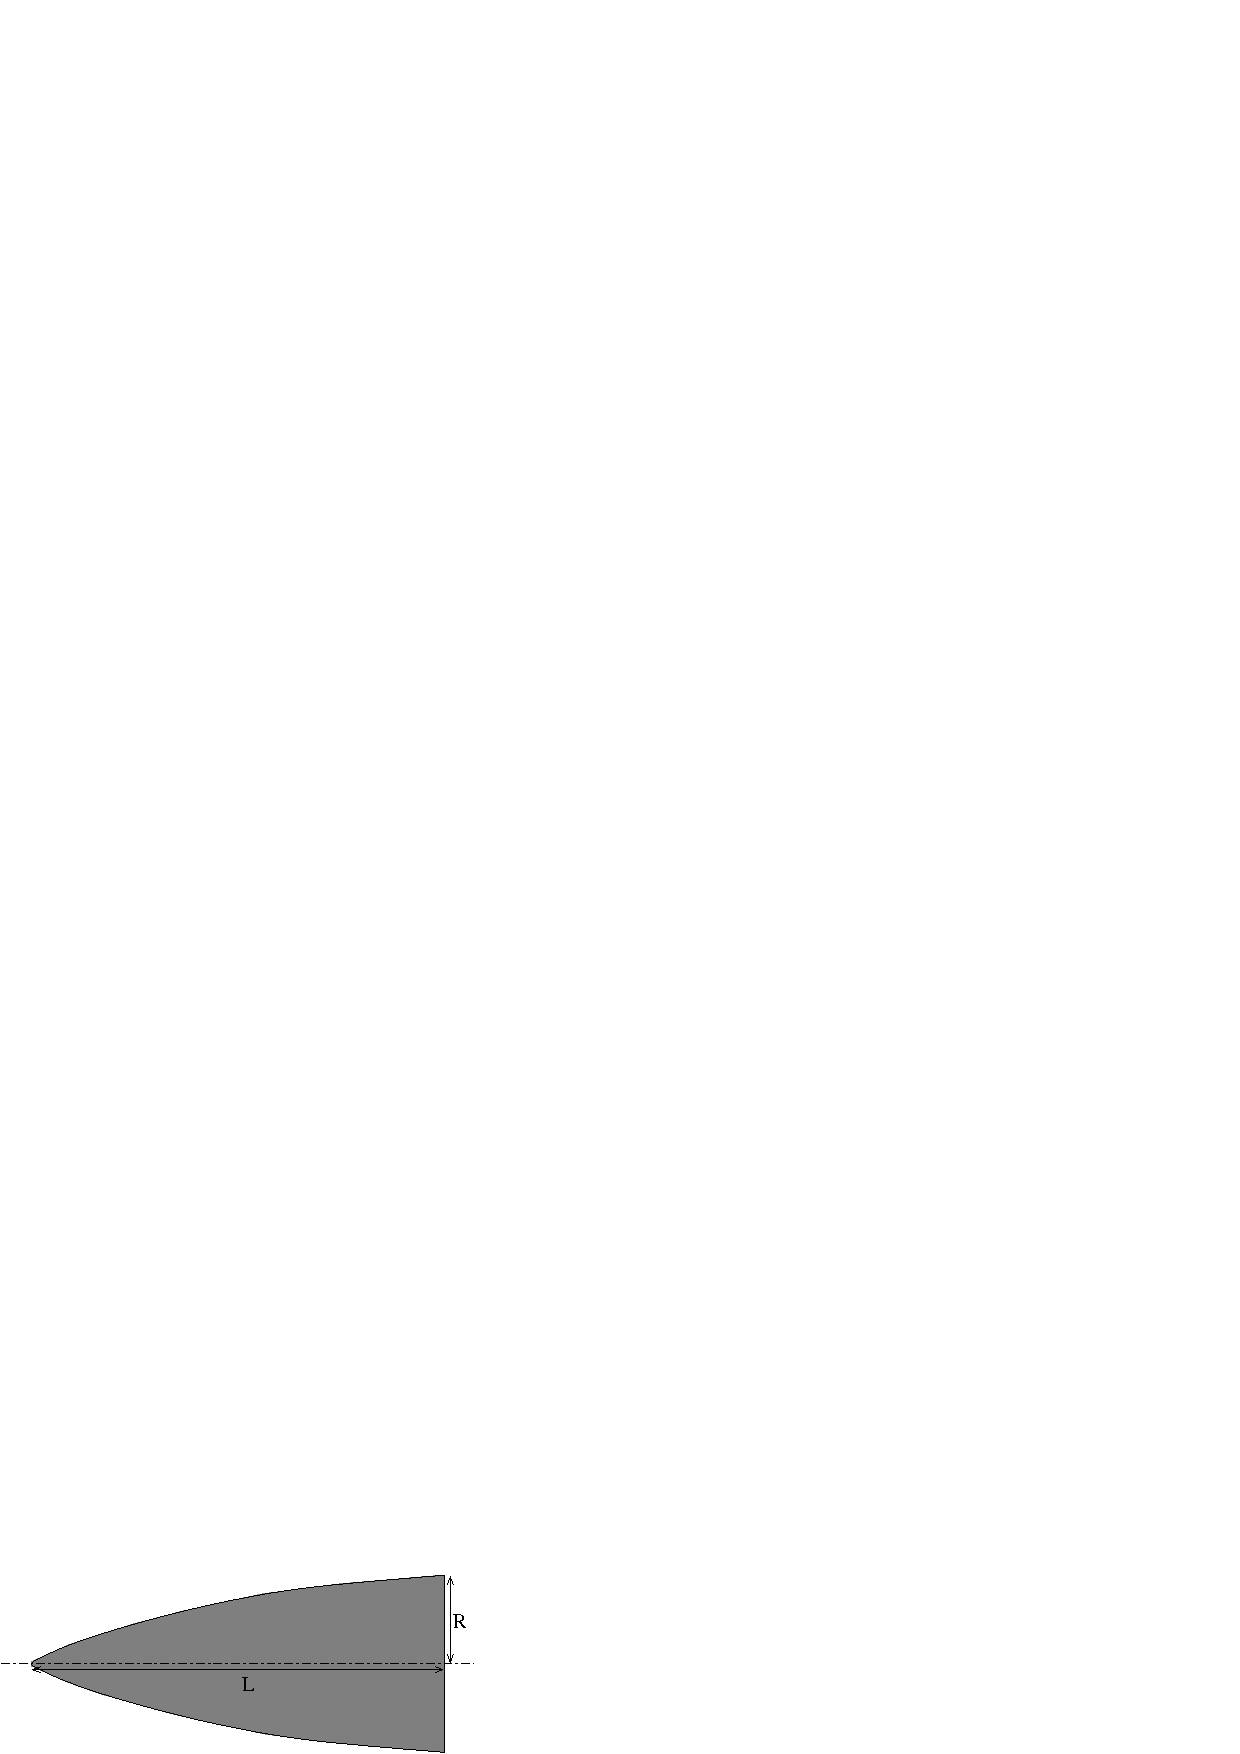
\epsfig{file=figures/nose-geometry/geometry-haack,scale=0.6} \\
(e) && (f) \\
&& \\
%&& \\
\end{tabular}
\caption{Various nose cone geometries:  (a)~conical, (b)~secant ogive,
  (c)~elliptical, (d)~parabolic, (e)~1/2~power (ellipsoid) and
  (f)~Haack series (Von K�rman).}
\label{fig-nosecone-shapes}
\end{figure}

\begin{figure}[p]
\vspace{5mm}
\begin{center}
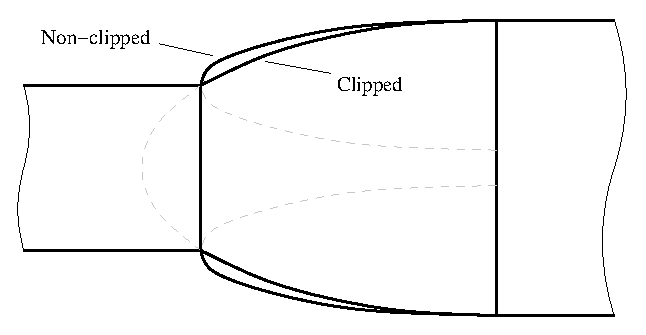
\epsfig{file=figures/nose-geometry/geometry-transition,scale=0.7}
\end{center}
\caption{A clipped and non-clipped elliptical transition.}
\label{fig-transition-clip}
\end{figure}





\chapter{Transonic wave drag of nose cones}
\label{app-nosecone-drag-method}

The wave drag of different types of nose cones vary largely in the
transonic velocity region.  Each cone shape has its distinct
properties.  In this appendix methods for calculating and
interpolating the drag of various nose cone shapes at transonic and
supersonic speeds are presented.  A summary of the methods is
presented in Appendix~\ref{app-transonic-nosecone-summary}.



\section{Blunt cylinder}
\label{app-blunt-cylinder-drag}

A blunt cylinder is the limiting case for every nose cone shape at the
limit $f_N\rightarrow 0$.  Therefore it is useful to have a formula
for the front pressure drag of a circular cylinder in longitudinal
flow.  As the object is not streamline, its drag coefficient does not
vary according to the Prandtl factor~(\ref{eq-prandtl-factor}).
Instead, the coefficient is approximately proportional to the
{\it stagnation pressure}, or the pressure at areas perpendicular to
the airflow.  The stagnation pressure can be approximated by the
function~\cite[pp.~15-2,~16-3]{hoerner}
%
\begin{equation}
\frac{q_{\rm stag}}{q} =
\left\{
\begin{array}{ll}
1 + \frac{M^2}{4} + \frac{M^4}{40}, & \mbox{for\ } M < 1 \\
1.84 - \frac{0.76}{M^2} + \frac{0.166}{M^4} + \frac{0.035}{M^6}, &
   \mbox{for\ } M > 1
\end{array}
\right. .
\end{equation}
%
The pressure drag coefficient of a blunt circular cylinder as a
function of the Mach number can then be written as
%
\begin{equation}
(C_{D\bullet})_{\rm pressure} = 
(C_{D\bullet})_{\rm stag} = 0.85 \cdot \frac{q_{\rm stag}}{q}.
\label{eq-blunt-cylinder-drag}
\end{equation}





\section{Conical nose cone}

A conical nose cone is simple to construct and closely resembles many
slender nose cones.  The conical shape is also the limit of several
parametrized nose cone shapes, in particular the secant ogive with
parameter value 0.0 (infinite circle radius), the power series nose
cone with parameter value 1.0 and the parabolic series with parameter
value 0.0.

Much experimental data is available on the wave drag of conical nose
cones.  Hoerner presents formulae for the value of $C_{D\bullet}$ at
supersonic speeds, the derivative  $\dif C_{D\bullet}/\dif M$ at
$M=1$,  and a figure of $C_{D\bullet}$ at
$M=1$~\cite[pp.~16-18\ldots16-20]{hoerner}.  Based on these and 
the low subsonic drag coefficient~(\ref{eq-nosecone-pressure-drag}), a
good interpolation of the transonic region is possible.

The equations presented by Hoerner are given as a function of the
half-apex angle $\varepsilon$, that is, the angle between the conical
body and the body centerline.  The half-apex angle is related to the
nose cone fineness ratio by
%
\begin{equation}
\tan\varepsilon = \frac{d/2}{l} = \frac{1}{2f_N}.
\end{equation}

The pressure drag coefficient at supersonic speeds ($M\gtrsim1.3$) is
given by
%
\begin{align}
(C_{D\bullet})_{\rm pressure}
& =  2.1\;\sin^2\varepsilon + 0.5\;
                 \frac{\sin\varepsilon}{\sqrt{M^2-1}} \nonumber\\
& =  \frac{2.1}{1+4f_N^2} + \frac{0.5}{\sqrt{(1+4f_N^2)\; (M^2-1)}} .
\label{eq-conical-supersonic-drag}
\end{align}
%
It is worth noting that as the Mach number increases, the drag
coefficient tends to the constant value $2.1\sin^2\epsilon$.  At $M=1$
the slope of the pressure drag coefficient is equal to
%
\begin{equation}
\eval{\frac{\partial (C_{D\bullet})_{\rm pressure}}{\partial M}}_{M=1} =
  \frac{4}{\gamma+1} \cdot (1-0.5\;C_{D\bullet,M=1})
\label{eq-conical-sonic-drag-derivative}
\end{equation}
%
where $\gamma=1.4$ is the specific heat ratio of air and the drag
coefficient at $M=1$ is approximately
%
\begin{equation}
C_{D\bullet,M=1} = 1.0\; \sin\varepsilon.
\label{eq-conical-sonic-drag}
\end{equation}

The pressure drag coefficient between Mach~0 and Mach~1 is
interpolated using equation~(\ref{eq-nosecone-pressure-drag}).  
Between Mach~1 and Mach~1.3 the coefficient is calculated using
polynomial interpolation with the boundary conditions from
equations~(\ref{eq-conical-supersonic-drag}),
(\ref{eq-conical-sonic-drag-derivative}) and
(\ref{eq-conical-sonic-drag}).






\section{Ellipsoidal, power, parabolic and Haack series nose cones}
\label{app-haack-series-pressure-drag}

A comprehensive data set of the pressure drag coefficient for all nose
cone shapes at all fineness ratios at all Mach numbers is not
available.  However, Stoney has collected a compendium of nose cone
drag data including data on the effect of the fineness ratio $f_N$ on
the drag coefficient and an extensive study of drag coefficients of
different nose cone shapes at fineness ratio
3~\cite{nosecone-cd-data}.  The same report suggests that the effects 
of fineness ratio and Mach number may be separated.

The curves of the pressure drag coefficient as a function of the nose
fineness ratio $f_N$ can be closely fitted with a function of the form
%
\begin{equation}
(C_{D\bullet})_{\rm pressure} = \frac{a}{(f_N + 1)^b}.
\label{eq-fineness-ratio-drag-interpolator}
\end{equation}
%
The parameters $a$ and $b$ can be calculated from two data points
corresponding to fineness ratios 0 (blunt cylinder,
Appendix~\ref{app-blunt-cylinder-drag}) and ratio 3.  Stoney includes
experimental data of the pressure drag coefficient as a function of
Mach number at fineness ratio 3 for power series $x^{1/4}$, $x^{1/2}$,
$x^{3/4}$ shapes, $1/2$, $3/4$ and full parabolic shapes, ellipsoidal,
L-V~Haack and Von K�rman nose cones.  These curves are written into
the software as data curve points.  For parametrized nose cone shapes
the necessary curve is interpolated if 
necessary.  Typical nose cones of model rockets have fineness ratios
in the region of 2--5, so the extrapolation from data of fineness
ratio 3 is within reasonable bounds.





\section{Ogive nose cones}

One notable shape missing from the data in Stoney's report are secant
and tangent ogives.  These are common shapes for model rocket nose
cones.  However, no similar experimental data of the pressure drag as
a function of Mach number was found for ogive nose cones.

At supersonic velocities the drag of a tangent ogive is approximately
the same as the drag of a conical nose cone with the same length and
diameter, while secant ogives have a somewhat smaller
drag~\cite[p.~239]{handbook-supersonic-aerodynamics}.  The minimum
drag is achieved when the secant ogive radius is approximately twice
that of a corresponding tangent ogive, corresponding to the parameter
value 0.5.  The minimum drag is consistently 18\% less than that of a
conical nose at Mach numbers in the range of 1.6--2.5 and for fineness
ratios of 2.0--3.5.  Since no better transonic data is available, it
is assumed that ogives follow the conical drag profile through
the transonic and supersonic region.  The drag of the corresponding
conical nose is diminished in a parabolic fashion with the ogive
parameter, with a minimum of -18\% at a parameter value of 0.5.





\section{Summary of nose cone drag calculation}
\label{app-transonic-nosecone-summary}

The low subsonic pressure drag of nose cones is calculated using
equation~(\ref{eq-nosecone-pressure-drag}):
%
\begin{equation*}
(C_{D\bullet,M=0})_p = 0.8 \cdot \sin^2\phi.
\end{equation*}
%
The high subsonic region is interpolated using a function of the form
presented in equation~(\ref{eq-nosecone-pressure-interpolator}):
%
\begin{equation*}
(C_{D\bullet})_{\rm pressure} = a\cdot M^b + (C_{D\bullet,M=0})_p
\end{equation*}
%
where $a$ and $b$ are selected according to the lower boundary of the
transonic pressure drag and its derivative.

The transonic and supersonic pressure drag is calculated depending on
the nose cone shape as follows:
%
\begin{itemize}

\item[\bf Conical:]  At supersonic velocities ($M > 1.3$) the
  pressure drag is calculated using
  equation~(\ref{eq-conical-supersonic-drag}).  Between Mach 1 and 1.3
  the drag is interpolated using a polynomial with boundary conditions
  given by equations~(\ref{eq-conical-supersonic-drag}),
  (\ref{eq-conical-sonic-drag-derivative}) and
  (\ref{eq-conical-sonic-drag}).
\\



\item[\bf Ogival:]  The pressure drag at transonic and supersonic
  velocities is equal to the pressure drag of a conical nose cone with
  the same diameter and length corrected with a shape factor:
%, multiplied by the shape factor
%
\begin{equation}
(C_{D\bullet})_{\rm pressure} = 
\del{0.72 \cdot (\kappa - 0.5)^2 + 0.82} \cdot 
(C_{D\bullet})_{\rm cone}.
\end{equation}
%
The shape factor is one at $\kappa = 0, 1$ and 0.82 at $\kappa=0.5$.
\\



\item[\bf Other shapes:]  The pressure drag calculation is based on
  experimental data curves:
%
\begin{enumerate}
\item Determine the pressure drag $C_3$ of a similar nose cone
  with fineness ratio $f_N=3$ from experimental data.  If data for a
  particular shape parameter is not available, interpolate the data
  between parameter values.

\item Calculate the pressure drag of a blunt cylinder $C_0$
  using equation~(\ref{eq-blunt-cylinder-drag}).

\item Interpolate the pressure drag of the nose cone using
  equation~(\ref{eq-fineness-ratio-drag-interpolator}).
  After parameter substitution the equation takes the form
%
\begin{equation}
(C_{D\bullet})_{\rm pressure} \;=\;
\frac{C_0}{(f_N+1)^{\log_4 C_0/C_3}} \;=\;
C_0 \cdot \del{\frac{C_3}{C_0}}^{\log_4(f_N+1)}
\end{equation}
%
  The last form is computationally more efficient since the exponent
  $\log_4(f_N+1)$ is constant during a simulation.

\end{enumerate}

\end{itemize}











\chapter{Streamer drag coefficient estimation}
\label{app-streamers}


A streamer is a typically rectangular strip of plastic or other
material that is used as a recovery device especially in small model
rockets.  The deceleration is based on the material flapping in the
passing air, thus causing air resistance.  Streamer optimization has
been a subject of much interest in the rocketry
community~\cite{streamer-optimization}, and contests on streamer
landing duration are organized regularly.  In order to estimate the
drag force of a streamer a series of experiments were performed and an
empirical formula for the drag coefficient was developed.

One aspect that is not taken into account in the present investigation
is the fluctuation between the streamer and rocket.  At one extreme a
rocket with a very small streamer drops head first to the ground with
almost no deceleration at all.  At the other extreme there is a very
large streamer creating significant drag, and the rocket falls below
it tail-first.  Between these two extremes is a point where the
orientation is labile, and the rocket as a whole twirls
around during descent.  This kind of interaction between the rocket
and streamer cannot be investigated in a wind tunnel and would require
an extensive set of flight tests to measure.  Therefore it is not
taken into account, instead, the rocket is considered effectively a
point mass at the end of the streamer, the second extreme mentioned
above.


\subsubsection*{Experimental methods}

A series of experiments to measure the drag coefficients of streamers
was performed using the $40\times40\times120$~cm wind tunnel of
Pollux~\cite{pollux-wind-tunnel}.  The experiments were performed
using various materials, widths and lengths of streamers and at
different wind speeds.  The effect of the streamer size and shape was
tested separately from the effect of the streamer material.

A tube with a rounded $90^\circ$ angle at one end was installed in the
center of the wind tunnel test section.  A line was drawn through the
tube so that one end of the line was attached to a the streamer and the
other end to a weight which was placed on a digital scale.  When the
wind tunnel was active the force produced by the streamer was read
from the scale.  A metal wire was taped to the edge of the streamer to
keep it rigid and the line attached to the midpoint of the wire.

A few different positions within the test section and free line
lengths were tried.  All positions seemed to produce approximately
equal results, but the variability was significantly lower when the
streamer fit totally into the test section and had a only 10~cm length
of free line between the tube and streamer.  This configuration was
used for the rest of the experiments.

Each streamer was measured at three different velocities, 6~m/s, 9~m/s
and 12~m/s.  The results indicated that the force produced is
approximately proportional to the square of the airspeed, signifying
that the definition of a drag coefficient is valid also for streamers.

The natural reference area for a streamer is the area of the strip.
However, since in the simulation we are interested in the total drag
produced by a streamer, it is better to first produce an equation for
the drag coefficient normalized to unit area, $C_D \cdot \Aref$.
These coefficient values were calculated separately for the different
velocities and then averaged to obtain the final normalized drag
coefficient of the streamer.


\subsubsection*{Effect of streamer shape}

\begin{figure}[p]
\centering
\hspace*{-7mm}
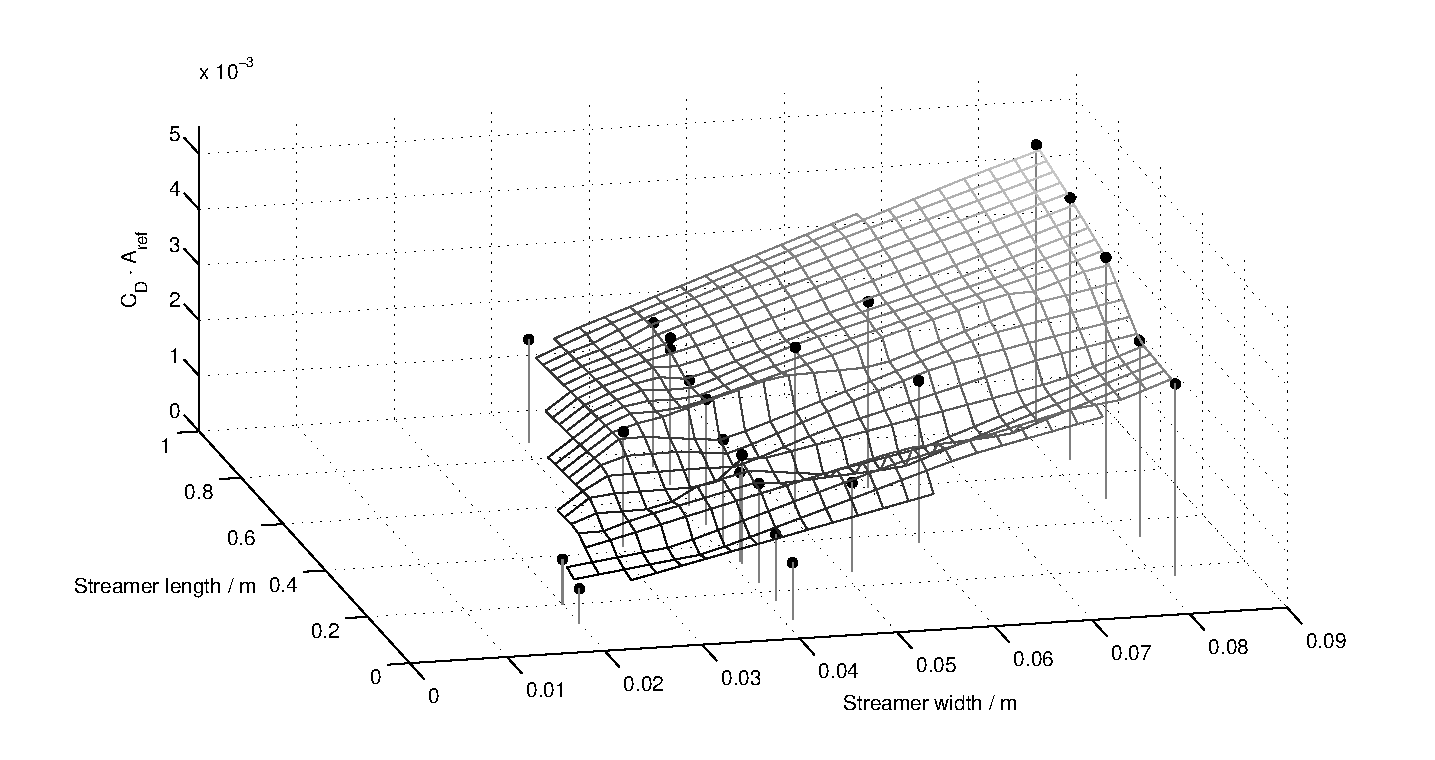
\epsfig{file=figures/experimental/streamerCDvsWL,width=155mm}
\caption{The normalized drag coefficient of a streamer as a function
  of the width and length of the streamer.  The points are the
  measured values and the mesh is cubically interpolated between the
  points.}
\label{fig-streamer-CD-vs-shape}
\end{figure}


\begin{figure}[p]
\centering
\hspace*{-7mm}
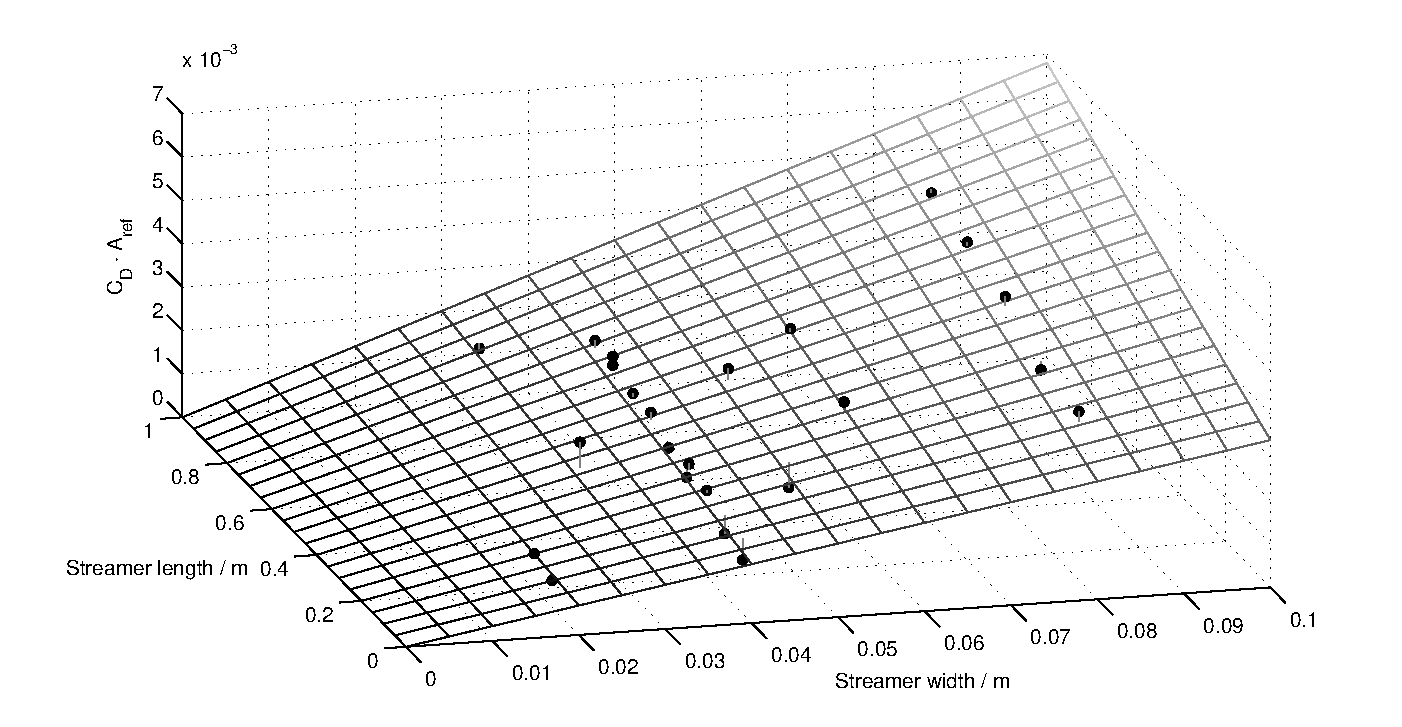
\epsfig{file=figures/experimental/streamerCDvsWLestimate,width=155mm}
\caption{Estimated and measured normalized drag coefficients of a
  streamer as a function of the width and length of the streamer.  The
  lines from the points lead to their respective estimate values.}
\label{fig-streamer-shape-estimate}
\end{figure}



Figure~\ref{fig-streamer-CD-vs-shape} presents the normalized drag
coefficient as a function of the streamer width and length for a fixed
material of $\rm80~g/m^2$ polyethylene plastic.  It was noticed that
for a specific streamer length, the normalized drag coefficient was
approximately linear with the width,
%
\begin{equation}
C_D \cdot \Aref = k\cdot w,
\label{eq-streamer-first-approx}
\end{equation}
%
where $w$ is the width and $k$ is dependent on the streamer length.
The slope $k$ was found to be approximately linear with
the length of the streamer, with a linear regression of
%
\begin{equation}
k = 0.034 \cdot (l+\rm 1~m).
\label{eq-streamer-second-approx}
\end{equation}
%
Substituting equation (\ref{eq-streamer-second-approx}) into
(\ref{eq-streamer-first-approx}) yields
%
\begin{equation}
C_D \cdot \Aref = 0.034 \cdot (l+{\rm 1~m})\cdot w
\label{eq-streamer-estimate}
\end{equation}
%
or using $\Aref = wl$
%
\begin{equation}
C_D = 0.034 \cdot \frac{l+\rm 1~m}{l}.
\label{eq-streamer-shape-estimate}
\end{equation}


The estimate as a function of the width and length is presented in 
Figure~\ref{fig-streamer-shape-estimate} along with the measured data
points.  The lines originating from the points lead to their
respective estimate values.  The average relative error produced by
the estimate was 9.7\%.


\subsubsection*{Effect of streamer material}



The effect of the streamer material was studied by creating
$4\times40$~cm and $8\times48$~cm streamers from various household
materials commonly used in streamers.  The tested materials were
polyethylene plastic of various thicknesses, cellophane and cr�pe
paper.  The properties of the materials are listed in
Table~\ref{table-streamer-materials}. 


Figure~\ref{fig-streamer-material} presents the normalized drag
coefficient as a function of the material thickness and surface
density.  It is evident that the thickness is not a good
parameter to characterize the drag of a streamer.  On the other hand,
the drag coefficient as a function of surface density is nearly
linear, even including the cr�pe paper.  While it is not as
definitive, both lines seem to intersect with the $x$-axis at
approximately  $\rm-25~g/m^2$.  Therefore the coefficient of the
$\rm80~g/m^2$ polyethylene estimated by
equation~(\ref{eq-streamer-shape-estimate}) is corrected for a
material surface density $\rho_m$ with
%
\begin{equation}
C_{D_m} = \left(\frac{\rho_m + \rm 25~g/m^2}{\rm 105~g/m^2}\right)
    \cdot C_D.
\end{equation}
%
Combining these two equations, one obtains the final empirical
equation
%
\begin{equation}
C_{D_m} = 0.034 \cdot
    \left(\frac{\rho_m + \rm 25~g/m^2}{\rm 105~g/m^2}\right) \cdot
    \left(\frac{l + 1~{\rm m}}{l}\right).
\label{eq-streamer-CD-estimate}
\end{equation}

This equation is also reasonable since it produces positive and finite
normalized drag coefficients for all values of $w$, $l$ and $\rho_m$.
However, this equation does not obey the rule-of-thumb of rocketeers
that the optimum width-to-length ratio for a streamer would be 1:10.
According to equation~(\ref{eq-streamer-estimate}), the maximum drag
for a fixed surface area is obtained at the limit $l\rightarrow0$,
$w\rightarrow\infty$.  In practice the rocket dimensions limit the
practical dimensions of a streamer, from which the 1:10 rule-of-thumb
may arise.


\subsubsection*{Equation validation}

To test the validity of the equation, several additional streamers
were measured for their drag coefficients.  These were of various
materials and of dimensions that were not used in the fitting of the
empirical formulae.  These can therefore be used as an independent
test set for validating equation~(\ref{eq-streamer-CD-estimate}).

Table~\ref{table-streamer-validation} presents the tested streamers
and their measured and estimated normalized drag coefficients.  The
results show relative errors in the range of 12--27\%.  While rather
high, they are considered a good result for estimating such a random
and dynamic process as a streamer.  Furthermore, due to the
proportionality to the square of the velocity, a 25\% error in the
normalized force coefficient translates to a 10--15\% error in the
rocket's descent velocity.  This still allows the rocket designer to
get a good estimate on how fast a rocket will descend with a
particular streamer.


\begin{figure}[p]
\centering
\parbox{70mm}{\centering
\epsfig{file=figures/experimental/streamerCDvsThickness2,width=70mm}
\\ (a)
}\parbox{70mm}{\centering
\epsfig{file=figures/experimental/streamerCDvsDensity2,width=70mm} \\ (b)}
\caption{The normalized drag coefficient of a streamer as a function
  of (a) the material thickness and (b) the material surface density.}
\label{fig-streamer-material}
\end{figure}



\begin{table}[p]
\caption{Properties of the streamer materials experimented with.}
\label{table-streamer-materials}
\begin{center}
\begin{tabular}{ccc}
\hline
Material & Thickness / \um & Density / $\rm g/m^2$ \\
\hline
Polyethylene & 21 & 19 \\
Polyethylene & 22 & 10 \\
Polyethylene & 42 & 41 \\
Polyethylene & 86 & 80 \\
Cellophane   & 20 & 18 \\
Cr�pe paper  & 110$\dagger$ & 24 \\
\hline
\end{tabular} \\
{\footnotesize $\dagger$ Dependent on the amount of pressure applied.}
\end{center}
\end{table}



\begin{table}[p]
\caption{Streamers used in validation and their results.}
\label{table-streamer-validation}
\begin{center}
\begin{tabular}{ccccccc}
\hline
Material & Width & Length & Density & Measured & Estimate & Error \\
         & m     & m      & $\rm g/m^2$ &
  \multicolumn{2}{c}{$10^{-3} (C_D\cdot\Aref)$} &  \\
\hline
Polyethylene & 0.07 & 0.21 & 21 & 0.99 & 1.26 & 27\% \\
Polyethylene & 0.07 & 0.49 & 41 & 1.81 & 2.23 & 23\% \\
Polyethylene & 0.08 & 0.24 & 10 & 0.89 & 1.12 & 26\% \\
Cellophane   & 0.06 & 0.70 & 20 & 1.78 & 1.49 & 17\% \\
Cr�pe paper  & 0.06 & 0.50 & 24 & 1.27 & 1.43 & 12\% \\
\hline
\end{tabular}
\end{center}
\end{table}






\end{document}
